\documentclass[11pt,a4paper]{article}
\usepackage[T1]{fontenc}
\usepackage[english]{babel}
\usepackage[hmargin=24mm,vmargin=24mm]{geometry}
\usepackage{amsmath,amssymb,amsthm}
\usepackage{booktabs,tabularx,array}
\usepackage{graphicx}
\usepackage{xcolor}
\usepackage{tikz}
\usetikzlibrary{arrows.meta,positioning,calc}
\usepackage[hidelinks,pdftitle={One Object, Three Frames: The Quantum Sphaera Construction},pdfauthor={Marc Brendecke}]{hyperref}

% Status colours (same as the figures)
\definecolor{st-est}{HTML}{3A7A3A}   % established
\definecolor{st-cond}{HTML}{A08000}  % conditional
\definecolor{st-read}{HTML}{55559A}  % reading
\definecolor{st-ref}{HTML}{9A3030}   % refuted
\definecolor{st-open}{HTML}{B0601A}  % open

% Status tags used in the running text
\newcommand{\Established}{\textsf{\textcolor{st-est}{[established]}}}
\newcommand{\Conditional}{\textsf{\textcolor{st-cond}{[conditional]}}}
\newcommand{\Reading}{\textsf{\textcolor{st-read}{[reading]}}}
\newcommand{\Refuted}{\textsf{\textcolor{st-ref}{[refuted]}}}
\newcommand{\Open}{\textsf{\textcolor{st-open}{[open]}}}
\newcommand{\Exploration}{\textsf{\textcolor{st-read}{[exploration]}}}

% Companion references: \rnd{r12} = round v4.10.0-r12; \rndold{r84} = round v4.9.0-r84
\newcommand{\rnd}[1]{\textsc{c}\,#1}
\newcommand{\rndold}[1]{\textsc{c}\,4.9-#1}

\theoremstyle{plain}
\newtheorem{proposition}{Proposition}[section]
\newtheorem{lemma}[proposition]{Lemma}
\theoremstyle{definition}
\newtheorem{definition}[proposition]{Definition}
\theoremstyle{remark}
\newtheorem{remark}[proposition]{Remark}

\newcommand{\tr}{\operatorname{tr}}
\newcommand{\bsym}{\beta_{\mathrm{sym}}}

\setlength{\parindent}{1em}
\raggedbottom
\emergencystretch=3em

\InputIfFileExists{release-info}{}{\def\releaseline{Draft\enspace$\cdot$\enspace November 2026}}
\begin{document}
\thispagestyle{plain}
\noindent{\LARGE\bfseries One Object, Three Frames:\\[0.2em] The Quantum Sphaera Construction\par}
\vspace{0.7em}
\noindent Marc Brendecke\hfill{\small\releaseline}\par
\vspace{0.8em}
\begin{quote}
\small
\noindent\textbf{Abstract.}
The Quantum Sphaera construction starts from a conjecture: matter, light and a tachyon sector are one object seen from three
frames. Its carrier is a biquaternion kernel built from three complex kernels, split by a compensator $C=\tfrac12(1+J)$ into
symmetric and antisymmetric parts; the sign of the field invariant $s=z_1^2+z_2^2+z_3^2$ separates the sectors. This article
reports what the construction establishes, what it assumes, and where it stops. The carrier, the compensator, the sector rule
and the frame maps are established mathematics; the tachyon map $z\mapsto iz$ is electromagnetic duality, distinct from time
reversal, and frame maps yield equalities, not values. On $\mathbb C\otimes\mathbb H\otimes\mathbb O$ one generation and the
Standard Model gauge group follow under named choices; the Albert algebra carries a family $SO(3)$ that the charge operator
breaks exactly to $A_4$, and, under a placeholder charge axis, a relative CP sign of leptons and quarks is fixed; one further
setting turns it into the open prediction $\sin\delta_{\rm PMNS}<0$. Read as the spectrum of a Gram matrix, Koide's relation is
equivalent to a mean squared overlap $\tfrac12$ of three states, whose extremal configuration is the octant; the overlap itself is
an input, so $K=\tfrac23$ is not derived. Later tests trace this input to a postulated exchange symmetry of the
matter and the tachyon frame and leave the Koide phase a fit. The numerical values offered for the open problems go back to one
frame offset, $\bsym\approx0.549$, each through a separately set identification; it follows from a horizon counting rule that is adopted as a postulate and not derived. A common action of Einstein--Cartan type with Dixon-stored fermions and a Higgs field, set up by author decisions, gives
consistent field equations but no scale; within the present stock no equation selects $\Lambda$. No lepton masses, no number of
generations, no absolute scale and no value of $\Lambda$ are derived, and no blind prediction has so far been confirmed against
measurement data. The open problems OP1--OP5 and the testable statements are listed with their
status. The authoritative source of every statement is the Quantum Sphaera Companion~\cite{QSC}.
\end{quote}

\tableofcontents
\section{Introduction}
\label{sec:A-intro}

\subsection{The conjecture}
\label{sec:A-conjecture}

The Quantum Sphaera construction starts from one conjecture: \emph{matter, light and a tachyon
sector are one object, seen from three frames.} In the Companion~\cite{QSC} this is the central
statement \texttt{thm:unity}. The object is a biquaternion kernel built from three complex kernels,
and a projector, the Heisenberg compensator, splits every state into a part that an involution keeps
and a part that it reverses. Matter, light and the tachyon sector are meant to be sectors of this one
kernel, and the frames are meant to be the views in which each sector is seen.

The conjecture has a history that a reader should know. In its first form, ``the same object'' meant
unitary equivalence, and the equivalence was argued from a Stone--von Neumann theorem taken from an
earlier Riemann-hypothesis manuscript of the author. That justification was withdrawn in round
v4.8.0-r04, and the statement has the status of a conjecture since then \Open. What survives today
is more modest and more precise. On the complex three-vector $z=\mathbf E+i\mathbf B$ the Lorentz
group and the electromagnetic duality rotation act, and their orbits are the shells $|s|=r>0$ of the
invariant $s=z\cdot z$, the punctured null cone and the origin (v4.8.0-r07; \rnd{r16}). A matter-type
and a tachyon-type configuration with the same $|s|$ lie on one orbit; light lies on another and is
reached from the first only as a limit (\rnd{r21}). So ``one object'' holds in the sense of an active
symmetry between matter and tachyon \Established, while the physical identification of the sectors
with matter, light and tachyons, and the claim that they are one physical state, remain a \Reading.
Sections~\ref{sec:A-carrier} and~\ref{sec:A-frames} make this precise.

\subsection{What this article does}
\label{sec:A-what}

This article reports the construction as it stands at Companion round v4.10.0-r60. It does not
present a deductive framework. For each result it says which of five kinds it is:
\begin{itemize}
\item \Established: mathematics with a proof, or a computation that anyone can repeat.
\item \Conditional: holds under named choices, settings or assumptions, which are stated with it.
\item \Reading: an interpretation of established mathematics. It may guide work but carries no proof
  weight; \Exploration{} marks results of explorations without a pre-registered criterion.
\item \Open: a question that is posed and not answered.
\item \Refuted: a pre-registered test whose criterion failed. Refuted tests appear only where they ground
  a result of the section in which they stand.
\end{itemize}
The tags are attached in the text where a statement is made. Figure~\ref{fig:A-overview} shows the
construction as a map with the same colours.

\paragraph{How the evidence is organised.}
The Companion grows in \emph{rounds}. A round is appended to the source and never rewritten;
corrections come as new rounds that name what they correct. We cite round v4.10.0-r$NN$ as
\rnd{r$NN$} and round v4.9.0-r$NN$ as \rndold{r$NN$}; rounds of the earlier v4.8.0 line are cited
by their full name, and labels of the Companion main text in typewriter font, e.g.\
(\cite{QSC}, \texttt{prop:compensator}). A test with a decision criterion is written down and committed
as a pre-registered note before the computation, and receives a number H$NN$. When the outcome could
be seen analytically before the computation, the Companion marks the test \emph{not blind}; such a test
checks a computation, not a prediction. Work without a pre-registered criterion is called an
exploration. The bookkeeping of statements, their premises and the guards that block unproved
conclusions is described in a separate article on the QAM language; here we use only its outcome, the
status of each statement.

\paragraph{What is not derived.}
We state this up front because it shapes every later section. The construction derives no particle
mass, no absolute scale and no value of the cosmological constant $\Lambda$. Where a number appears,
such as the frame offset $\bsym\approx0.549$, it is inserted, and we say so. The Koide value $K=2/3$
is not derived: Section~\ref{sec:B-koide} shows that it is equivalent to an overlap $\tfrac12$ between three states,
and that overlap is an input. Against external measurements there is, so far, no confirmed blind
prediction. A review at round \rnd{r05} counted about 20 confirmed, 19 refuted, 9 invalid, 4 open and
28 mixed test outcomes since v4.8.0, 29 of them marked not blind; the confirmed tests without that
mark all check inner mathematics \cite{QSC}. The predictions that are still pending, with their
deadlines, are listed in Section~\ref{sec:open}.

\paragraph{What the construction does supply.}
It supplies exact statements about a carrier and its symmetries: a projector and its image, a sign
rule for three sectors, two field classes under the Lorentz group, duality and scale, the action of
three frame maps, conditions under which three readout states form an octant, and conditional
constructions of one particle generation. It also supplies exclusions: several routes from the
structure to numbers are closed by proofs or refuted tests. We regard both as results.

% F1: overview map of the construction, status at Companion round v4.10.0-r60.
% 2.5D: three stacked layers (carrier, frames and sectors, readouts) drawn as slanted planes with shadows.
% Node fill and edge colour carry the status; a text tag and the line style repeat it for black-and-white print.
\begin{figure}[t]
\centering
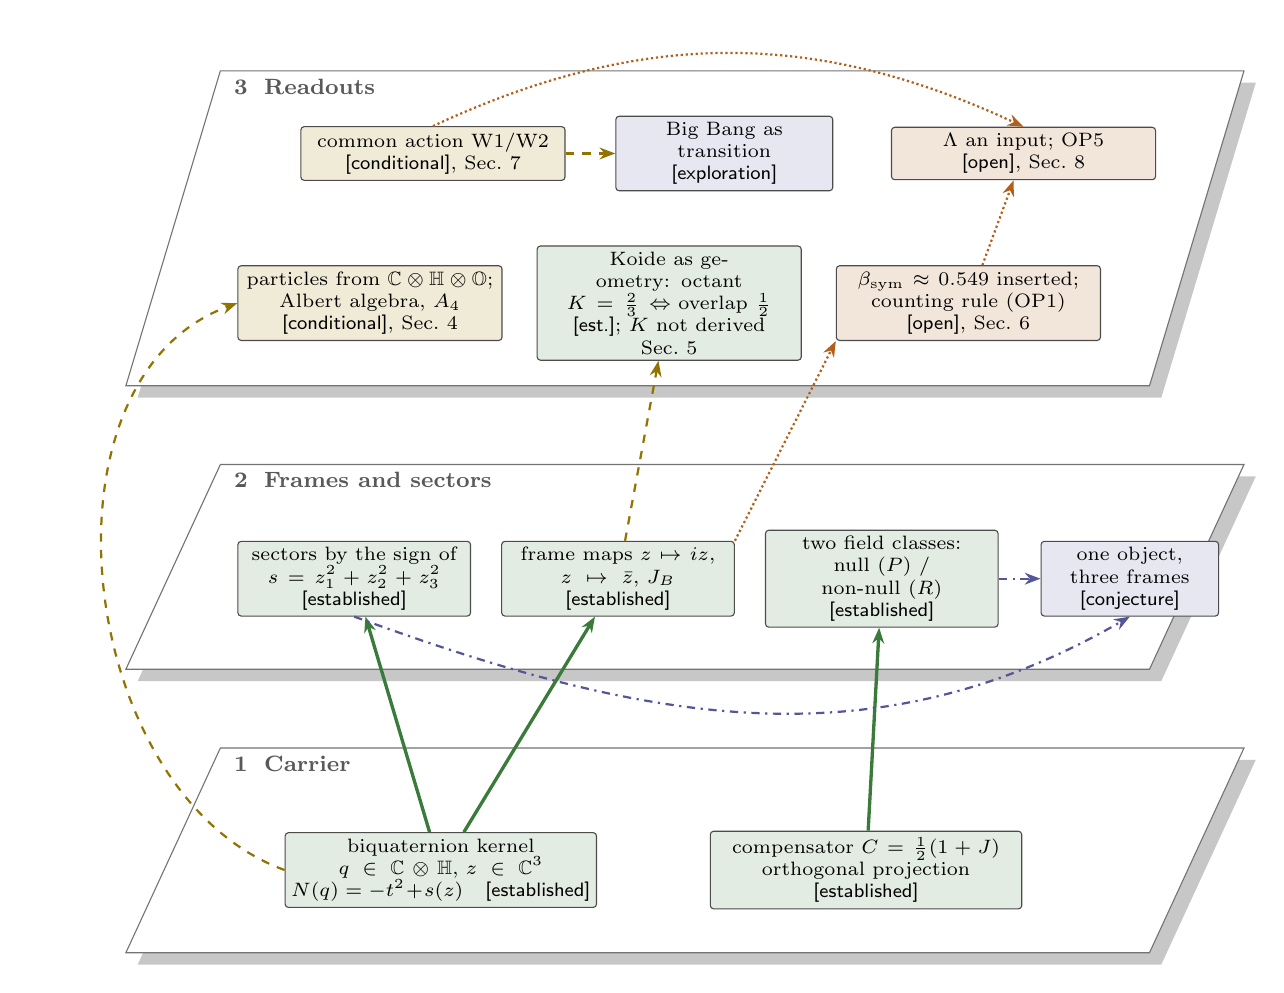
\begin{tikzpicture}[
  font=\scriptsize,
  box/.style={draw=black!70, rounded corners=1.2pt, align=center, inner sep=2.2pt, text width=#1},
  box/.default=3.2cm,
  est/.style={fill=st-est!14},
  cond/.style={fill=st-cond!16},
  read/.style={fill=st-read!14},
  open/.style={fill=st-open!16},
  ref/.style={fill=st-ref!14},
  eest/.style={-{Stealth[length=2mm]}, very thick, draw=st-est},
  econd/.style={-{Stealth[length=2mm]}, thick, dashed, draw=st-cond!90!black},
  eopen/.style={-{Stealth[length=2mm]}, thick, densely dotted, draw=st-open},
  eread/.style={-{Stealth[length=2mm]}, thick, dash dot, draw=st-read},
]
% ---------- layer planes (drawn first, back to front) ----------
\newcommand{\qsplane}[3]{% #1 = y offset, #2 = height, #3 = label
  \fill[black!22] (0.15,#1-0.15) -- (13.15,#1-0.15) -- (14.35,#1+#2-0.15) -- (1.35,#1+#2-0.15) -- cycle;
  \filldraw[fill=white, draw=black!55] (0,#1) -- (13,#1) -- (14.2,#1+#2) -- (1.2,#1+#2) -- cycle;
  \node[anchor=south west, font=\footnotesize\bfseries, text=black!65] at (1.25,#1+#2-0.42) {#3};}
\qsplane{7.2}{4.0}{3 \;Readouts}
\qsplane{3.6}{2.6}{2 \;Frames and sectors}
\qsplane{0}{2.6}{1 \;Carrier}

% ---------- layer 1: carrier ----------
\node[box=3.8cm, est] (kern) at (4.0,1.05)
  {biquaternion kernel\\ $q\in\mathbb C\otimes\mathbb H$, $z\in\mathbb C^3$\\ $N(q)=-t^2+s(z)$\quad\textsf{[established]}};
\node[box=3.8cm, est] (comp) at (9.4,1.05)
  {compensator $C=\tfrac12(1+J)$\\ orthogonal projection\\ \textsf{[established]}};

% ---------- layer 2: frames and sectors ----------
\node[box=2.8cm, est] (sect) at (2.9,4.75)
  {sectors by the sign of\\ $s=z_1^2+z_2^2+z_3^2$\\ \textsf{[established]}};
\node[box=2.8cm, est] (maps) at (6.25,4.75)
  {frame maps $z\mapsto iz$,\\ $z\mapsto\bar z$, $J_B$\\ \textsf{[established]}};
\node[box=2.8cm, est] (class) at (9.6,4.75)
  {two field classes:\\ null ($P$) / non-null ($R$)\\ \textsf{[established]}};
\node[box=2.1cm, read] (unity) at (12.75,4.75)
  {one object,\\ three frames\\ \textsf{[conjecture]}};

% ---------- layer 3: readouts ----------
\node[box=3.2cm, cond] (part) at (3.1,8.25)
  {particles from $\mathbb C\otimes\mathbb H\otimes\mathbb O$;\\ Albert algebra, $A_4$\\ \textsf{[conditional]}, Sec.~4};
\node[box=3.2cm, est] (koide) at (6.9,8.25)
  {Koide as geometry: octant\\ $K=\tfrac23\Leftrightarrow$ overlap $\tfrac12$\\ \textsf{[est.]}; $K$ not derived\\ Sec.~5};
\node[box=3.2cm, open] (beta) at (10.7,8.25)
  {$\beta_{\rm sym}\approx0.549$ inserted;\\ counting rule (OP1)\\ \textsf{[open]}, Sec.~6};
\node[box=3.2cm, cond] (act) at (3.9,10.15)
  {common action W1/W2\\ \textsf{[conditional]}, Sec.~7};
\node[box=2.6cm, read] (bang) at (7.6,10.15)
  {Big Bang as transition\\ \textsf{[exploration]}};
\node[box=3.2cm, open] (lam) at (11.4,10.15)
  {$\Lambda$ an input; OP5\\ \textsf{[open]}, Sec.~8};

% ---------- edges ----------
\draw[eest] (kern) -- (sect);
\draw[eest] (kern) -- (maps);
\draw[eest] (comp) -- (class);
\draw[eread] (class) -- (unity);
\draw[eread] (sect.south) to[out=-20,in=-150] (unity.south);
\draw[econd] (kern.west) to[out=160,in=200] (part.west);
\draw[econd] (maps) -- (koide);
\draw[eopen] (maps.north east) -- (beta.south west);
\draw[econd] (act) -- (bang);
\draw[eopen] (act.north) to[out=25,in=155] (lam.north);
\draw[eopen] (beta) -- (lam);
\end{tikzpicture}

\smallskip
\begin{tabular}{@{}l@{\quad}l@{\quad}l@{\quad}l@{}}
\tikz\draw[-{Stealth[length=1.6mm]},very thick,st-est] (0,0)--(0.7,0); established &
\tikz\draw[-{Stealth[length=1.6mm]},thick,dashed,st-cond!90!black] (0,0)--(0.7,0); conditional &
\tikz\draw[-{Stealth[length=1.6mm]},thick,densely dotted,st-open] (0,0)--(0.7,0); open &
\tikz\draw[-{Stealth[length=1.6mm]},thick,dash dot,st-read] (0,0)--(0.7,0); reading
\end{tabular}
\caption{Overview of the construction at Companion round \rnd{r60}. The bottom layer is
the carrier (Section~\ref{sec:A-carrier}), the middle layer the sectors, frame maps and the two field
classes (Section~\ref{sec:A-frames}), the top layer the physical readouts treated in Sections~4--8.
Fill colour, text tag and line style give the status of each node and link. Green: proved
mathematics. Yellow: holds under named choices or settings. Orange: open. Blue: a reading,
conjecture or exploration. The established links into layer~2 are algebra; every arrow into
layer~3 carries a choice or an open step, and no arrow yields a mass, a scale or a value of
$\Lambda$.}
\label{fig:A-overview}
\end{figure}


\subsection{Plan of the article}
\label{sec:A-plan}

Section~\ref{sec:A-carrier} defines the carrier: the biquaternion kernel, the involution $J$ and the
compensator $C=\tfrac12(1+J)$, the sector rule by the sign of $s=z_1^2+z_2^2+z_3^2$, and what $C$
does to a light field. All of it is established mathematics; the names of the sectors are a reading.
Section~\ref{sec:A-frames} introduces the frames M, T, P and R of Convention~F and the maps between
them. The tachyon map $z\mapsto iz$ is the electromagnetic duality rotation, not a Wick rotation and
not time reversal $z\mapsto\bar z$. Under the Lorentz group, duality and scale there are exactly two
classes of non-zero fields, and frame maps, being symmetries, give equalities between frames and no
values. Section~\ref{sec:B-particles} constructs particles from $\mathbb C\otimes\mathbb H\otimes\mathbb O$ under named
choices, up to the family symmetry of the Albert algebra and its breaking to $A_4$. Section~\ref{sec:B-koide} treats
the Koide relation as geometry of three states and shows why it is not a derivation. Section~\ref{sec:beta} is about
the frame offset $\bsym$ and the counting rule behind it, the open problem OP1. Section~\ref{sec:act} presents the
common action W1/W2, which holds under author decisions and supplies no scale, together with a short
exploration of the Big Bang as a transition. Section~\ref{sec:lop5} collects the negative results on $\Lambda$ and
the open problem OP5. Section~\ref{sec:open} lists the open problems and the testable statements with their status,
and Section~\ref{sec:concl} concludes. Appendix~\ref{sec:ledger} gives the status ledger of every statement, Appendix~\ref{sec:repro} the scripts
that reproduce the numbers.

\section{Carrier, compensator and sectors}
\label{sec:A-carrier}

This section collects the mathematics on which everything else rests. All statements in it are
\Established, with proofs that fit on a few lines. The physical names attached to the objects
(matter, light, tachyon) are a \Reading{} and are marked as such.

\subsection{The biquaternion kernel}
\label{sec:A-kernel}

\begin{definition}[Biquaternion kernel; \cite{QSC}, \texttt{def:biquaternion}]
\label{def:A-kernel}
Let $e_1,e_2$ be imaginary quaternion units and $e_3=e_1e_2$. A kernel is a biquaternion
\begin{equation}
q=it\,\mathbf 1+z_1e_1+z_2e_2+z_3e_3\in\mathbb C\otimes_{\mathbb R}\mathbb H,
\qquad t\in\mathbb R,\quad z=(z_1,z_2,z_3)\in\mathbb C^3 .
\label{eq:A-kernel}
\end{equation}
The three complex coefficients $z_k$ are the three \emph{complex kernels} $K_1,K_2,K_3$ of the
construction. The complex unit $i$ commutes with the quaternion units.
\end{definition}

The original definition equipped $q$ with the Hermitian norm $-t^2+\sum_k|z_k|^2$ and read it as a
Minkowski metric. Round v4.8.0-r06 corrected this: as a real quadratic form in the seven real
variables $(t,\operatorname{Re}z_k,\operatorname{Im}z_k)$ it has signature $(1,6)$, and conjugation by
real unit quaternions only rotates $\operatorname{Re}z$ and $\operatorname{Im}z$, each by the same spatial rotation; it
contains no boost. The invariant that the algebra provides is a different one.

\begin{proposition}[Natural norm; v4.8.0-r06.1]
\label{prop:A-norm}
Let $\bar q=it\,\mathbf 1-z_1e_1-z_2e_2-z_3e_3$ be quaternion conjugation without complex
conjugation. Then
\begin{equation}
N(q):=q\bar q=-t^2+s(z),\qquad s(z)=z_1^2+z_2^2+z_3^2,
\label{eq:A-norm}
\end{equation}
and $N(pq)=N(p)N(q)$.
\end{proposition}

\begin{proof}
Write $q=it+\mathbf z$ with $\mathbf z=\sum_kz_ke_k$. The coefficients commute with the units, so
$q\bar q=(it)^2+it(-\mathbf z)+\mathbf z(it)-\mathbf z^2=-t^2-\mathbf z^2$. In
$\mathbf z^2=\sum_{j,k}z_jz_ke_je_k$ the mixed terms cancel because $e_je_k=-e_ke_j$ for $j\neq k$, and
$e_k^2=-1$ gives $\mathbf z^2=-s(z)$. Multiplicativity follows from $\overline{pq}=\bar q\,\bar p$ and
the fact that $N(q)$ is a scalar.
\end{proof}

The working reading of the kernel since v4.8.0-r06 (``Reading~B'', an author decision) takes $z$ as
the carrier of the Lorentz group: conjugation $q\mapsto uqu^{-1}$ with $u\in\mathbb C\otimes\mathbb H$,
$N(u)=1$, fixes the scalar part and acts on $z$ by $SO(3,\mathbb C)$, and
$SO(3,\mathbb C)\cong PSL(2,\mathbb C)\cong SO^+(1,3)$. In this reading $z$ is the
Riemann--Silberstein vector of an electromagnetic field \cite{A-BBB2013},
\begin{equation}
z=\mathbf E+i\mathbf B,\qquad
s=z\cdot z=|\mathbf E|^2-|\mathbf B|^2+2i\,\mathbf E\cdot\mathbf B ,
\label{eq:A-s}
\end{equation}
so that $s$ collects the two Lorentz invariants of the field (units with $c=1$). The scalar $t$ is
an invariant parameter, not the time coordinate of a four-vector. Its role is \Open; on the null set
$N(q)=0$ it would be tied to $s$ by $s=t^2$ (v4.8.0-r07), a candidate that has not been adopted.

The motivating ``triole'' of three kernels with equal moduli and phases $120^\circ$ apart also
finds an exact place here.

\begin{proposition}[Triole; v4.8.0-r06.2]
\label{prop:A-triole}
For $z\in\mathbb C^3$, $\;z_1+z_2+z_3=0$ and $s(z)=0$ hold together if and only if
$z=c\,(1,\omega,\omega^2)$ up to order, with $\omega=e^{2\pi i/3}$ and $c\in\mathbb C$.
\end{proposition}

\begin{proof}
With the elementary symmetric functions $e_1,e_2,e_3$ of the $z_k$ one has $s=e_1^2-2e_2$. So
$e_1=s=0$ gives $e_2=0$, and the $z_k$ are the roots of $\lambda^3-e_3$, the three cube roots of $e_3$.
Conversely $1+\omega+\omega^2=0$ and $1+\omega^2+\omega^4=0$.
\end{proof}

The triole is therefore a centred null configuration. Centring alone does not force $s=0$:
$z=(1,-1,0)$ is centred and has $s=2$.

\subsection{The compensator}
\label{sec:A-compensator}

The second ingredient is a projector built from an involution. Since round v4.8.0-r04 it is defined
and proved on its own, without reference to that earlier manuscript.

\begin{definition}[Heisenberg compensator; v4.8.0-r04.1]
\label{def:A-compensator}
Let $V$ be a real or complex Hilbert space and $J:V\to V$ a linear involution that is self-adjoint,
$J^2=1$, $J^*=J$ (equivalently, an orthogonal or unitary involution). The \emph{compensator} and its
partner are
\begin{equation}
C=\tfrac12(1+J),\qquad A=\tfrac12(1-J).
\label{eq:A-compensator}
\end{equation}
\end{definition}

\begin{proposition}[Compensator as orthogonal projection; v4.8.0-r04.2]
\label{prop:A-compensator}
$C$ and $A$ are complementary orthogonal projections: $C^2=C=C^*$, $A^2=A=A^*$, $CA=AC=0$, $C+A=1$.
Their ranges are $\operatorname{ran}C=\ker(J-1)$ and $\operatorname{ran}A=\ker(J+1)$, and
$C(Jf)=Cf$, $A(Jf)=-Af$ for all $f$.
\end{proposition}

\begin{proof}
$C^2=\tfrac14(1+2J+J^2)=\tfrac12(1+J)=C$, and $C^*=C$ because $J^*=J$; the same computation with $-J$
gives $A$. $CA=AC=\tfrac14(1-J^2)=0$ and $C+A=1$. From $JC=\tfrac12(J+1)=C$, $J$ acts as $1$ on
$\operatorname{ran}C$; conversely $Jf=f$ gives $Cf=f$. Hence $\operatorname{ran}C=\ker(J-1)$, and likewise
$JA=-A$ gives $\operatorname{ran}A=\ker(J+1)$. Finally $CJ=C$ and $AJ=-A$.
\end{proof}

So $C$ keeps the part of a state that $J$ leaves fixed and removes the part that $J$ reverses, and the
two parts are orthogonal. Nothing beyond $J^2=1$ and $J^*=J$ is used. The main-text statement
of \texttt{prop:compensator}, that $C$ ``takes matter and its tachyon image and produces the photon'',
does not follow from this; Section~\ref{sec:A-field-example} shows why.

\paragraph{The field instance.}
On the field $z=\mathbf E+i\mathbf B$ the involution used by the Companion is the exchange of
electric and magnetic field,
\begin{equation}
J_Bz=i\bar z,\qquad J_B(\mathbf E+i\mathbf B)=\mathbf B+i\mathbf E .
\label{eq:A-JB}
\end{equation}
On $\mathbb C^3$ it is antilinear, but on the real space of pairs $(\mathbf E,\mathbf B)\cong\mathbb R^6$
it is linear, orthogonal and symmetric, so Proposition~\ref{prop:A-compensator} applies over $\mathbb R$.
Writing the field as the real $3\times2$ matrix $F=[\,\mathbf E\mid\mathbf B\,]$, $J_B$ acts as
$F\mapsto F\sigma_x$ and the compensator as $F\mapsto FC_{\rm HC}$ with
$C_{\rm HC}=\tfrac12(1+\sigma_x)$ (\rndold{r04}). From \eqref{eq:A-compensator},
\begin{equation}
Cz=(1+i)\,\frac{\mathbf E+\mathbf B}{2},\qquad Az=(1-i)\,\frac{\mathbf E-\mathbf B}{2}.
\label{eq:A-Cz}
\end{equation}
In the kept part both field vectors are equal to $(\mathbf E+\mathbf B)/2$; in the removed part they
are opposite.

\subsection{Sectors by the sign of \texorpdfstring{$s$}{s}}
\label{sec:A-sectors}

The invariant $s$ sorts the field configurations. The following proposition is the exact content of
the sector rule.

\begin{proposition}[Orbits and sectors; v4.8.0-r06.3, r06.4, r07.1, r07.2]
\label{prop:A-orbits}
Let $SO(3,\mathbb C)$ act on $\mathbb C^3$ and let $U(1)_{\rm dual}$ act by $z\mapsto e^{i\alpha}z$.
\begin{enumerate}
\item[(a)] The $SO(3,\mathbb C)$-orbits are the level sets $\{s=c\}$ for $c\neq0$, the punctured null
  cone $\{s=0\}\setminus\{0\}$, and $\{0\}$.
\item[(b)] $s(e^{i\alpha}z)=e^{2i\alpha}s(z)$. In particular the quarter turn $z\mapsto iz$ maps
  $s\mapsto-s$ and preserves the null cone.
\item[(c)] Every $z$ with $s(z)\neq0$ is $z=e^{i\alpha}z_m$ with $s(z_m)=|s(z)|>0$; the angle
  $\alpha=\tfrac12\arg s(z)$ is fixed modulo $\pi$. The configuration has $s>0$ exactly for
  $\alpha\equiv0$ and $s<0$ exactly for $\alpha\equiv\pi/2\pmod\pi$.
\item[(d)] The orbits of $SO(3,\mathbb C)\times U(1)_{\rm dual}$ on $\mathbb C^3\setminus\{0\}$ are the
  shells $\{|s|=r\}$, $r>0$, and the punctured null cone. The null cone is the only orbit fixed by the
  whole duality circle.
\end{enumerate}
\end{proposition}

\begin{proof}
(a) $SO(3,\mathbb C)$ preserves the bilinear form, hence $s$. For $s\neq0$ put $e=z/\sqrt s$, complete
it to a complex-orthonormal basis of determinant one, and rotate $z$ to $(\sqrt s,0,0)$; so each level
set is one orbit. A non-zero null vector is $z(\psi)=(\psi_1^2-\psi_2^2,\;i(\psi_1^2+\psi_2^2),\;
-2\psi_1\psi_2)$ for a spinor $\psi\neq0$, unique up to sign, and the map is equivariant for
$SL(2,\mathbb C)\to SO(3,\mathbb C)$ (v4.8.0-r06.4); $SL(2,\mathbb C)$ is transitive on
$\mathbb C^2\setminus\{0\}$. (b) is immediate from bilinearity. (c) $s(e^{-i\alpha}z)=e^{-2i\alpha}s$ is
real and positive iff $2\alpha\equiv\arg s\pmod{2\pi}$. (d) combines (a) and (b): the duality circle
moves $s$ through all values of fixed modulus and fixes $s=0$.
\end{proof}

The Companion adopts the working assignment (v4.8.0-r07, author's choice)
\begin{equation}
s>0\ \text{matter},\qquad s=0\ \text{light},\qquad s<0\ \text{tachyon}.
\label{eq:A-assignment}
\end{equation}
On real $s$ the first case is electric dominance, the third magnetic dominance
(Figure~\ref{fig:A-sectors}). By (c), a configuration with non-real $s$ is not a further sector but a
matter configuration seen at a rotated duality angle. The assignment can be reversed without changing
any statement of Proposition~\ref{prop:A-orbits}; it is a \Reading. The projectivised null cone is a
smooth conic $\cong\mathbb CP^1\cong S^2$ (v4.8.0-r06.4), the space of directions of light-like
fields.

Two cautions belong here. First, $s$ is a field invariant, not the mass-shell invariant $p^2$ of a
particle momentum. The words ``matter'' and ``tachyon'' for the two signs therefore need a further
physical identification, which the construction does not supply. Second, by (d) matter and tachyon
configurations of equal $|s|$ lie on one orbit, but no invertible operation of the group connects a
configuration with $s\neq0$ to the null cone. A common orbit of all three types does not exist.

% F2: sectors of the field invariant s on the real slice E.B = 0 (3D, fixed perspective).
% Generated by scripts/F2_sectors.py -> figures/F2-sectors.pdf.  No data enter; the level c = 1 is a display choice.
\begin{figure}[t]
\centering
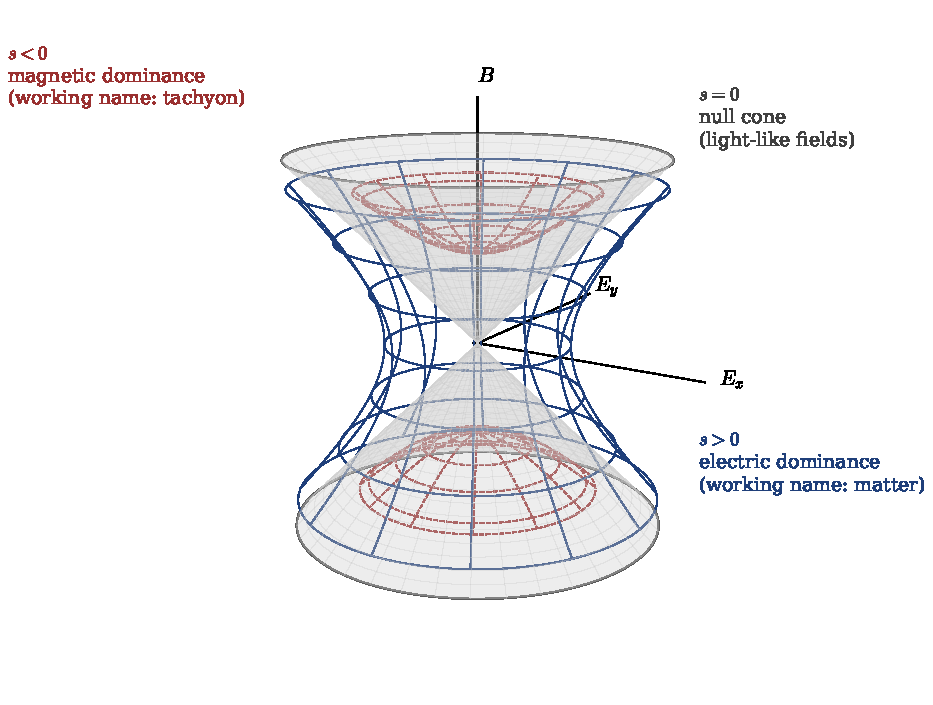
\includegraphics[width=0.78\textwidth]{figures/F2-sectors.pdf}
\caption{The three sectors of $s=z\cdot z$ on the slice where $\mathbf E\perp\mathbf B$, so that
$s=|\mathbf E|^2-|\mathbf B|^2$ is real ($\mathbf E$ horizontal, $\mathbf B$ vertical). Grey: the null cone
$s=0$ (light-like fields; the apex is the zero field). Solid: the level set $s=+1$ (electric dominance).
Dashed: the level set $s=-1$ (magnetic dominance). In the full space $\mathbb C^3$ the level sets
$s=c\neq0$ are the orbits of the Lorentz group $SO(3,\mathbb C)$, and the duality quarter turn
$z\mapsto iz$ maps the level $c$ to $-c$ (Proposition~\ref{prop:A-orbits}). The picture is a
three-dimensional slice of a six-dimensional space. \Established{} as geometry; the names matter and
tachyon are the working assignment of round v4.8.0-r07 and a \Reading.}
\label{fig:A-sectors}
\end{figure}


\subsection{What the compensator selects on a light field}
\label{sec:A-field-example}

The first test of a construction meant to describe light is a plane wave in vacuum: equal field
strengths and orthogonal fields. Take at one point $\mathbf E=a\mathbf e_x$, $\mathbf B=a\mathbf e_y$,
$a>0$, so $z=a(\mathbf e_x+i\mathbf e_y)$ and $s=0$. By \eqref{eq:A-Cz},
\begin{equation}
Cz=\frac a2(1+i)(\mathbf e_x+\mathbf e_y),\qquad Az=\frac a2(1-i)(\mathbf e_x-\mathbf e_y).
\label{eq:A-wave}
\end{equation}
The input has squared norm $|\mathbf E|^2+|\mathbf B|^2=2a^2$, each part has $a^2$; this is the
Pythagoras identity of the orthogonal splitting. The kept part has
$\mathbf E'=\mathbf B'=\tfrac a2(\mathbf e_x+\mathbf e_y)$, hence
$|\mathbf E'|^2=|\mathbf B'|^2=\mathbf E'\cdot\mathbf B'=a^2/2$ and
\begin{equation}
s(Cz)=2i\,|\mathbf E'|^2=i\,a^2\neq0 .
\label{eq:A-sC}
\end{equation}
The projection keeps the equality of the field strengths and destroys their orthogonality. The image
of a light-like field is not light-like.

This is general. For every field with $\mathbf E+\mathbf B\neq0$ the image $Cz$ has parallel electric
and magnetic parts, $\mathbf E'=\mathbf B'$. In the language of Section~\ref{sec:A-frames} it lies on
the rim $|b|=1$ of the state disk, the reference frame R, and never at the light-like centre P
(\rnd{r23}, Theoremlet r23.2) \Established. The kept and the removed part are each a selection; the
input is recovered only from both. A projection loses information, while symmetries do not
(\rnd{r16}, r16.6). The older reading of \texttt{prop:compensator}, in which $C$ produces the photon
from matter and its tachyon image, is therefore not supported: the quaternion identity $e_3=e_1e_2$
makes the \emph{product} $z\times J_Bz=2\,\mathbf E\times\mathbf B$ orthogonal to both inputs, not the
average (\rndold{r03}, r03.4). The Companion corrected the orthogonality clause of the proposition accordingly; its sentence
that $C$ produces the photon still stands in the main text and is superseded by \rnd{r23}.

\subsection{What the carrier does not give}
\label{sec:A-limits}

The carrier is a concrete algebra with checkable operations and invariants. It is not yet physics.
Four statements must be kept apart, and none implies the next: several data live on the same
mathematical carrier; several descriptions represent the same complete physical state; several states
belong to one theory and are connected by an active operation; different readouts of one state discard
different information. Proposition~\ref{prop:A-orbits} establishes the third for matter and tachyon
configurations; it says nothing about the second. The compensator is of the fourth kind.

In particular the carrier by itself identifies no particle. Which state is an electron and which a
photon requires the larger algebra
$\mathbb C\otimes\mathbb H\otimes\mathbb O$ and further named choices (Section~\ref{sec:B-particles}). The number of generations
is not derived there either; it is an input. It also contains
no dynamics: neither the evolution of $z$ nor an action that would fix a scale follows from the
algebra (Section~\ref{sec:act}). What it does fix is the frame structure of the next section.

\section{Frames and their maps}
\label{sec:A-frames}

The word ``frame'' carries the conjecture of Section~\ref{sec:A-intro}. This section fixes what it
means in the construction, which maps connect the frames, and what such maps can and cannot deliver.
The maps and their properties are \Established; the identification of frames with physical
observers of matter, light and tachyons is a \Reading.

\subsection{The field doublet and its state disk}
\label{sec:A-doublet}

Write the field as the real $3\times2$ matrix $F=[\,\mathbf E\mid\mathbf B\,]$ and form its Gram matrix
$G=F^{\mathsf T}F$ (\rndold{r04}). With $u=\tfrac12\operatorname{tr}G=\tfrac12(|\mathbf E|^2+|\mathbf B|^2)$ and
$s$ from \eqref{eq:A-s},
\begin{equation}
G=u\,\mathbf 1+\tfrac12\bigl(\operatorname{Re}s\;\sigma_z+\operatorname{Im}s\;\sigma_x\bigr),
\qquad \det G=|\mathbf E\times\mathbf B|^2,\qquad u^2-\det G=\tfrac14|s|^2 .
\label{eq:A-gram}
\end{equation}
For $u>0$ the normalised matrix $\rho=G/\operatorname{tr}G=\tfrac12(\mathbf 1+b_1\sigma_z+b_2\sigma_x)$
defines the \emph{state vector}
\begin{equation}
b=\frac{(\operatorname{Re}s,\operatorname{Im}s)}{2u},\qquad
|b|^2=1-\frac{\det G}{u^2}\le1 .
\label{eq:A-disk}
\end{equation}
The states fill a disk, not a sphere, because $G$ is real symmetric. Light-like fields ($s=0$) are
the centre $b=0$. The rim $|b|=1$ is reached exactly when $\mathbf E\parallel\mathbf B$. A boost leaves
$s$ fixed and changes $u$, so it moves $b$ along its own direction; for a non-null field it reaches
the rim in the frame where $\mathbf E\parallel\mathbf B$ and tends to the centre as the rapidity grows
(\rndold{r04}, r04.2). This is the Stokes formalism of polarisation optics, applied to the pair
$(\mathbf E,\mathbf B)$ instead of two polarisation components; the same three bases of the field
doublet appear in the literature \cite{A-Golat2024}.

\subsection{Convention F}
\label{sec:A-convention}

Since round \rndold{r22} every statement of the Companion carries the frame in which it holds. The
convention, completed in \rndold{r24} and corrected in \rndold{r28}, names four frames.
\begin{itemize}
\item \textbf{M}, the matter frame: the doublet state with eigenvalues $p_+=1/(1+x)$ in the compensator
  port and $p_-=x/(1+x)$ in the partner port, where $x=\bsym^2$.
\item \textbf{T}, the tachyon frame: the image of M under the tachyon map $z\mapsto iz$. It exchanges
  $p_+$ and $p_-$, sends $x\mapsto1/x$ and the frame factor $\gamma=(1+x)/(1-x)$ to $-\gamma$.
\item \textbf{P}, the photon eigenframe: the fixed point $b=0$, $p_+=p_-=\tfrac12$.
\item \textbf{R}, the reference frame: the pure state $|b|=1$, offset $\bsym=0$. It is the frame in
  which the Companion main text works; where older chapters say ``photon frame'' they mostly mean R.
\end{itemize}
A statement is \emph{frame-free} if M and T give the same value; otherwise it carries its frame. At P
a readout is evaluated separately and may be degenerate, and a degenerate value is not a global
statement. Quantities that depend on the state only through $|b|$ or the unordered pair of eigenvalues
(visibility, entropy) are frame-free; quantities that distinguish the two ports are matter-only
(\rndold{r22}, r22.1). The positions of M and T depend on the value of $\bsym$, which is inserted
(Section~\ref{sec:beta}); the convention itself does not.

\subsection{Three maps on the frame plane}
\label{sec:A-maps}

On the complex amplitude $z$, and in the Dixon algebra on its $\mathbb C$ factor (\rndold{r51}),
three involutive operations act. We write them as
\begin{equation}
\begin{aligned}
&D\colon z\mapsto iz &&\text{(tachyon map)},\\
&\vartheta\colon z\mapsto\bar z &&\text{(time reversal of the amplitudes)},\\
&J_B=D\circ\vartheta\colon z\mapsto i\bar z &&\text{(exchange of $\mathbf E$ and $\mathbf B$)}.
\end{aligned}
\label{eq:A-maps}
\end{equation}
On the frame plane $D$ is a rotation by $90^\circ$ and $\vartheta$ a reflection
(Figure~\ref{fig:A-frame-plane}). Strictly, $D$ squares to $-1$ on $z$; it is an involution on states,
where it acts as $\rho\mapsto\sigma_y\rho\sigma_y$. In the matrix picture $\vartheta$ is $F\mapsto F\sigma_z$,
$J_B$ is $F\mapsto F\sigma_x$, and $D$ is the rotation by $\pi/2$ in the column plane.

\begin{proposition}[Frame maps; v4.8.0-r06, \rndold{r04}, \rndold{r28}, \rnd{r07}]
\label{prop:A-maps}
\begin{enumerate}
\item[(a)] $s(Dz)=-s(z)$, $s(\vartheta z)=\overline{s(z)}$, and $s(J_Bz)=-\overline{s(z)}$. On the disk, $D$ sends
  $b\mapsto-b$, $\vartheta$ reverses $b_2$, and $J_B$ reverses $b_1$. All three keep $|b|$ and the null class.
\item[(b)] $D$ commutes with every $L\in SO(3,\mathbb C)$, that is, with all proper Lorentz transformations
  of the field.
\item[(c)] $\vartheta$ and $J_B$ commute with $L\in SO(3,\mathbb C)$ if and only if $L=\bar L$, that is, for
  spatial rotations only. A boost changes the form of the exchange rule.
\end{enumerate}
\end{proposition}

\begin{proof}
(a) $s$ is complex bilinear: $s(iz)=i^2s(z)$, $s(\bar z)=\overline{s(z)}$, and $s(i\bar z)=-\overline{s(z)}$. The
statements on $b$ follow from \eqref{eq:A-disk}, since $u$ is unchanged by all three maps. (b) $L$ is
complex linear, so $L(iz)=iLz$. (c) $L\vartheta z=L\bar z$ and $\vartheta Lz=\bar L\bar z$; these agree for all
$z$ iff $L=\bar L$. Real elements of $SO(3,\mathbb C)$ are the rotations. The same holds for $J_B=D\vartheta$
by (b).
\end{proof}

Three consequences need to be stated plainly, because earlier text of the Companion confused them.

\paragraph{The tachyon map is not time reversal.}
Both $D$ and $J_B$ reverse $\operatorname{Re}s$ and so send matter-type to tachyon-type configurations;
$\vartheta$ keeps $\operatorname{Re}s$. Convention~F as first written used $J_B$; round \rndold{r28}
corrected the tachyon map to $z\mapsto iz$, which in addition exchanges the compensator ports, and round \rndold{r51} showed that the charges $Q$ and $B-L$ and the chirality projectors of
the Dixon construction are fixed by $D$, so they are the same in M and T, whereas charge conjugation is
the time-reversal part $\vartheta$ \Established. Where earlier layers wrote ``frame T'' for charge conjugation,
time reversal was meant. The two maps must not be interchanged.

\paragraph{The tachyon map is electromagnetic duality, not a Wick rotation.}
With $z=\mathbf E+i\mathbf B$, $Dz$ is the duality rotation $\mathbf E\mapsto-\mathbf B$,
$\mathbf B\mapsto\mathbf E$, a map of field space and not of spacetime. By (b) it commutes with every
boost; a boost stays a boost with real rapidity. A remark in \rnd{r06} had asked whether $z\mapsto iz$
turns boosts into rotations and coincides with the Wick rotation $t\mapsto i\tau_E$; \rnd{r07} (Correction
r07.1) answered this in the negative \Established.

\paragraph{The names are a reading.}
That the orbit related by $D$ to a matter-type configuration is a physical tachyon, and that the null
class is light in the particle sense, is the working assignment \eqref{eq:A-assignment}. The maps
themselves are symmetries of the free Maxwell field (duality, Lorentz transformations) or a discrete
transformation of it (time reversal).

% F3: the frame plane and the state disk.  Tachyon map z -> iz (rotation by 90 deg) against time reversal z -> conj z
% (reflection) and J_B = i conj z.  2.5D: two stacked panels with shadows; the lower panel is the readout disk b.
% All positions are exact consequences of the maps: b(iz) = -b(z), b(conj z) = (b1,-b2), b(J_B z) = (-b1,b2)
% (Companion v4.9.0-r04.2(b),(c), v4.9.0-r28).
\begin{figure}[t]
\centering
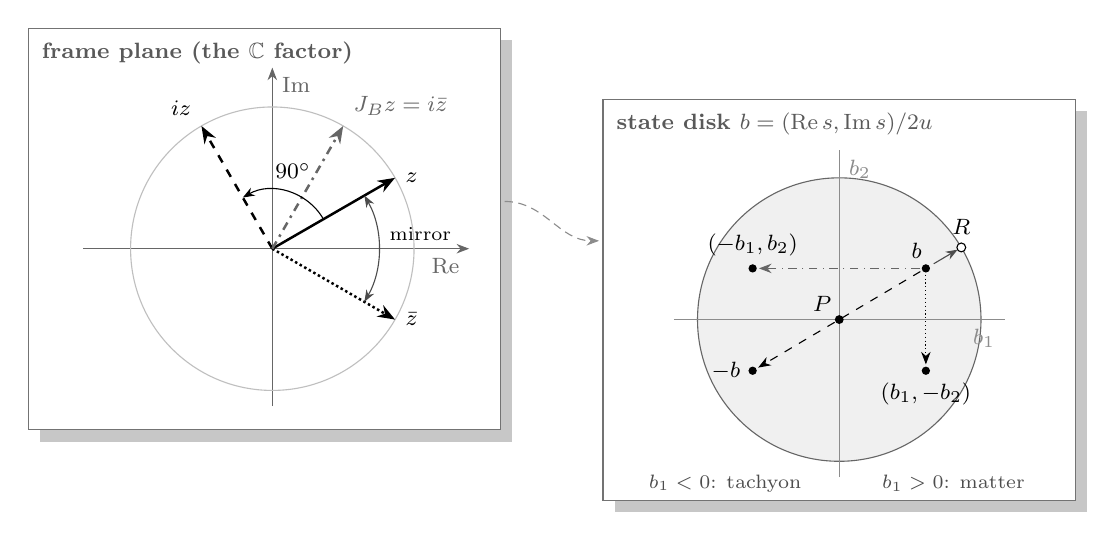
\begin{tikzpicture}[
  font=\footnotesize,
  vec/.style={-{Stealth[length=2.2mm]}, line width=0.9pt},
  panel/.style={fill=white, draw=black!55},
  shadow/.style={fill=black!22},
]
% ---------------- upper panel: the frame plane ----------------
\begin{scope}
  \fill[shadow] (-2.95,-2.45) rectangle (3.05,2.65);
  \filldraw[panel] (-3.1,-2.3) rectangle (2.9,2.8);
  \node[anchor=north west, font=\footnotesize\bfseries, text=black!65] at (-3.05,2.75) {frame plane (the $\mathbb C$ factor)};
  \draw[-{Stealth[length=1.6mm]}, black!60] (-2.4,0) -- (2.5,0) node[below left] {$\operatorname{Re}$};
  \draw[-{Stealth[length=1.6mm]}, black!60] (0,-2.0) -- (0,2.3) node[below right] {$\operatorname{Im}$};
  \draw[black!25] (0,0) circle (1.8);
  % z at 30 deg, iz at 120 deg, conj z at -30 deg, J_B z = i conj z at 60 deg
  \draw[vec, black] (0,0) -- (30:1.8) node[right] {$z$};
  \draw[vec, black, dashed] (0,0) -- (120:1.8) node[above left] {$iz$};
  \draw[vec, black, densely dotted] (0,0) -- (-30:1.8) node[right] {$\bar z$};
  \draw[vec, black!60, dash dot] (0,0) -- (60:1.8) node[above right] {$J_Bz=i\bar z$};
  \draw[-{Stealth[length=1.5mm]}, black] (30:0.75) arc (30:120:0.75);
  \node at (75:1.02) {$90^\circ$};
  \draw[{Stealth[length=1.5mm]}-{Stealth[length=1.5mm]}, black!70] (30:1.35) arc (30:-30:1.35);
  \node[right] at (8:1.38) {\scriptsize mirror};
\end{scope}
% ---------------- lower panel: the state disk ----------------
\begin{scope}[xshift=7.2cm, yshift=-0.9cm]
  \fill[shadow] (-2.85,-2.45) rectangle (3.15,2.65);
  \filldraw[panel] (-3.0,-2.3) rectangle (3.0,2.8);
  \node[anchor=north west, font=\footnotesize\bfseries, text=black!65] at (-2.95,2.75) {state disk $b=(\operatorname{Re}s,\operatorname{Im}s)/2u$};
  \fill[black!6] (0,0) circle (1.8);
  \draw[black!60] (0,0) circle (1.8);
  \draw[black!45] (-2.1,0) -- (2.1,0) node[below left] {$b_1$};
  \draw[black!45] (0,-2.0) -- (0,2.15) node[below right] {$b_2$};
  \node[font=\scriptsize, text=black!70, align=center] at (1.45,-2.08) {$b_1>0$: matter};
  \node[font=\scriptsize, text=black!70, align=center] at (-1.45,-2.08) {$b_1<0$: tachyon};
  % P at centre; a boost moves b radially to the rim (frame R)
  \fill (0,0) circle (1.6pt) node[above left=-1pt] {$P$};
  \draw[-{Stealth[length=1.5mm]}, black!70] (1.2,0.709) -- (1.503,0.888);
  \draw[fill=white] (1.550,0.916) circle (1.6pt) node[above=1pt] {$R$};
  % sample state b and its images
  \fill (1.1,0.65) circle (1.5pt) node[above left=0pt and -2pt] {$b$};
  \fill (-1.1,-0.65) circle (1.5pt) node[left=1pt] {$-b$};
  \fill (1.1,-0.65) circle (1.5pt) node[below=1pt] {$(b_1,-b_2)$};
  \fill (-1.1,0.65) circle (1.5pt) node[above=1pt] {$(-b_1,b_2)$};
  \draw[-{Stealth[length=1.6mm]}, dashed] (1.03,0.61) -- (-1.03,-0.61);
  \draw[-{Stealth[length=1.6mm]}, densely dotted] (1.1,0.57) -- (1.1,-0.57);
  \draw[-{Stealth[length=1.6mm]}, dash dot, black!60] (1.02,0.65) -- (-1.02,0.65);
\end{scope}
% connector between the panels
\draw[black!45, densely dashed, -{Stealth[length=1.6mm]}] (2.95,0.6) to[out=0,in=180] (4.15,0.1);
\end{tikzpicture}
\caption{The frame maps on the frame plane (left) and on the readout disk of the field doublet (right).
The tachyon map $z\mapsto iz$ (dashed) is a rotation by $90^\circ$; on the disk it is the point
reflection $b\mapsto-b$. Time reversal of the amplitudes $z\mapsto\bar z$ (dotted) is a mirror image;
on the disk it reverses $b_2$. Their composite $J_B z=i\bar z$ (dash-dotted) reverses $b_1$. Light-like
fields sit at the centre $P$ in every frame; a boost moves a non-null state along its own direction
and reaches the rim $|b|=1$, the frame $R$ with $\mathbf E\parallel\mathbf B$, at a finite rapidity.
\Established{} for the maps and their action \cite{QSC} (\rndold{r04}, \rndold{r28}, \rndold{r51}).}
\label{fig:A-frame-plane}
\end{figure}


\subsection{Exactly two classes of fields}
\label{sec:A-classes}

If one divides out not only the Lorentz group and duality but also the overall scale, the sector
structure collapses to a single predicate.

\begin{proposition}[Two classes; \rnd{r21}, r21.8]
\label{prop:A-classes}
Let $SO(3,\mathbb C)$ act on $z$ and let $\lambda\in\mathbb C\setminus\{0\}$ act by $z\mapsto\lambda z$ (duality
phase and dilation).
\begin{enumerate}
\item[(a)] All non-null fields form one orbit: for $s(z_1),s(z_2)\neq0$ there are $\lambda$ and $L$ with
  $z_2=\lambda Lz_1$.
\item[(b)] The non-zero null fields form one orbit, already of $SO(3,\mathbb C)$ alone.
\item[(c)] Each class has a distinguished representative. A non-null field is taken by a finite boost to
  the frame with $\mathbf E\parallel\mathbf B$, where $\phi:=|b|=1$; this is R. A null field has $\phi=0$ in
  every frame; this is P. On the first class boosts reach every $\phi\in(0,1]$; on the second only $0$.
\item[(d)] The rapidity $\eta_R$ of the boost from a field to R satisfies $\phi=\operatorname{sech}2\eta_R$.
\end{enumerate}
\end{proposition}

\begin{proof}
(a) Choose $\lambda$ with $\lambda^2s(z_1)=s(z_2)$; then $\lambda z_1$ and $z_2$ have the same $s$ and lie on
one $SO(3,\mathbb C)$-orbit by Proposition~\ref{prop:A-orbits}(a). (b) is Proposition~\ref{prop:A-orbits}(a)
for the null cone. (c) and (d): $s$ is fixed and $\phi=|s|/2u$; along the boost line $u$ takes every value
in $[|s|/2,\infty)$, with the minimum where $\det G=0$, i.e.\ $\mathbf E\parallel\mathbf B$; for $s=0$,
$\phi=0$ identically. The relation (d) was checked numerically on 1000 fields in \rnd{r21}.
\end{proof}

Below every frame-dependent readout there is therefore one frame-free predicate: whether a field is
null or not \Established. The port shares, the offset and the value of $\phi$ are readouts of a
frame above it. This is the precise sense in which matter and tachyon are ``one'' and light is
``another'': the first two lie in one class, light in the other, and no finite boost connects them.

\subsection{The collapse state, typed}
\label{sec:A-collapse}

The oldest formulation of the conjecture calls the common object the \emph{collapse state}
$z^-=0$ (\texttt{thm:unity}). Round \rnd{r22} typed all 93 occurrences of $z^-$ in the main text against
Convention~F \Reading. As a point, $z^-=0$ is in about two thirds of the places the zero of the offset,
that is R. The role of the frame-invariant object, which the same theorem ascribes to $z^-=0$, belongs to
P, and the main text places P, without naming it so, at the other end of its coordinate, $z^-\to\infty$
at $\beta\to1$, the horizon. The coordinate thus runs from R to P along the line
$\phi=\operatorname{sech}2\eta_R$ of Proposition~\ref{prop:A-classes}(d). The null class, the answer to
the question whether a field is null at the lowest level, is the horizon end of the main-text coordinate,
not its origin.

The same split resolves where the main-text ``cascade'' leads (\rnd{r23}). Two cascades carry one name.
The compensator cascade ends at R: every image $Cz$ with $\mathbf E+\mathbf B\neq0$ has $\phi=1$
(Section~\ref{sec:A-field-example}). The transport of the null axis keeps null fields null and so carries
P without leading there. No finite cascade in the source leads to P; only limits (boosts, dephasing over
many frequencies, weak coupling to a reservoir) or, for an instant, free time evolution reach it.

\subsection{Frame maps give equalities, not values}
\label{sec:A-equalities}

A symmetry between frames can show that two frames agree. It cannot supply the number on which they
agree. The clearest example in the Companion concerns gravity.

Dorau and Much derived the semiclassical Einstein equations from quantum relative entropy
\cite{A-DorauMuch2026}, a quantum field theoretic form of Jacobson's argument
\cite{A-Jacobson1995}. Near a point, with a local Rindler horizon, the relative entropy of a coherent
excitation equals an energy flux; with the Raychaudhuri equation and the area law $S_{\rm rel}=\delta A/4$,
which is assumed, one obtains $G_{ab}+\Lambda g_{ab}=8\pi\langle{:}T_{ab}{:}\rangle$, with $\Lambda$ an
integration constant. Round \rnd{r06} recorded this; round \rnd{r07} mapped the chain onto the frames
\Exploration{} (not blind):

\begin{proposition}[Frame-blind gravity for the Maxwell field; \rnd{r07}, r07.2]
\label{prop:A-frameblind}
For the free Maxwell field the relative-entropy chain gives in frame T the same Einstein equation as in
frame M, with the same coupling, sign and inputs.
\end{proposition}

\begin{proof}[Sketch]
The duality rotation is a symmetry of the free Maxwell field: it maps the algebra of the Rindler wedge
onto itself and fixes the vacuum. It commutes with boosts (Proposition~\ref{prop:A-maps}(b)), hence with
the modular group of the vacuum. Relative entropy is invariant under such an automorphism. The
energy--momentum tensor is Hermitian in $z$ (energy density $\tfrac12|z|^2$, Poynting vector
$(\bar z\times z)/2i$), so the null flux $T_{ab}\xi^a\xi^b$ is unchanged, while the bilinear invariants
$|\mathbf E|^2-|\mathbf B|^2$ and $\mathbf E\cdot\mathbf B$ change sign. The commutation and the invariance of
the tensor were checked numerically on 2000 random fields and boosts (script
\texttt{k217\_dualitaet\_gravitation.py}).
\end{proof}

Gravity couples to the Hermitian tensor; the frames differ in the bilinear invariants. For the Maxwell
field gravity is therefore frame-blind. This is textbook duality invariance in a new bookkeeping, not
new physics. Its limits are explicit: for massive fields the tachyon image of the action has no stable
Hadamard ground state, and the premises of the chain fail; for interacting fields duality is in general
not a symmetry.

The more important lesson is structural (\rnd{r07}, r07.4). The frame map is a symmetry that fixes the
reference state, and every link of the chain is invariant under it; such an argument yields equalities
between frames and nothing about the shared value. The prefactor of the area law is an absolute number.
The two horizon countings the Companion uses are each calibrated to the area law, and their ratio
$\gamma_L=\gamma_{\rm BI}/\gamma_{\rm string}=1.864700$ is independent of the normalisation, which cancels.
Every quantity the Companion builds from the two countings, including $\bsym$ (Section~\ref{sec:beta}), is exactly the
part in which the normalisation drops out. Neither Newton's constant nor $\Lambda$ follows
\Established.

\subsection{Orientation of the octant}
\label{sec:A-orientation}

One further property of the maps is used in Section~\ref{sec:B-koide}. On the Lorentz-invariant doublet
$\chi=(\sqrt{s_+},\sqrt{s_-})$ built from the helicity parts $F_\pm=\mathbf E\pm i\mathbf B$ of a field with
complex amplitudes (\rnd{r16}), the eigenstates of the frame maps form octant triples of three states with
pairwise overlap $\tfrac12$; the eight triples split into two orbits, one for each sign of the Bargmann phase
$\pm\pi/4$. The pre-registered test H118 (\rnd{r31}, partly not blind) found that the three frame maps, acting
linearly on the complex amplitudes, preserve this orientation, and so does parity, which exchanges $s_+$
and $s_-$. Time reversal of the complex field amplitudes, $\mathbf E\mapsto\bar{\mathbf E}$,
$\mathbf B\mapsto-\bar{\mathbf B}$, acts on $\chi$ as complex conjugation and reverses it. None of nine candidates listed beforehand
selects one orientation. The sign of the octant step is therefore a time orientation of the readout and is
not fixed by the construction \Open. Section~\ref{sec:B-koide} returns to this.

\subsection{Summary}
\label{sec:A-frames-summary}

\begin{table}[h]
\centering\small
\begin{tabularx}{\textwidth}{@{}>{\raggedright\arraybackslash}X l l@{}}
\toprule
statement & status & source\\
\midrule
natural norm $N(q)=-t^2+s(z)$; Lorentz action on $z$ (Reading~B) & \Established & v4.8.0-r06\\
compensator $C=\tfrac12(1+J)$ is an orthogonal projection & \Established & v4.8.0-r04\\
orbits and sector rule by the sign of $s$ & \Established & v4.8.0-r06, r07\\
names matter / light / tachyon for $s>0$, $=0$, $<0$ & \Reading & v4.8.0-r07\\
image of $C$ never light-like; lies at R & \Established & \rnd{r23}\\
$z\mapsto iz$ is duality, commutes with boosts; not a Wick rotation & \Established & \rnd{r07}\\
tachyon map $\neq$ time reversal; charges frame-free between M and T & \Established & \rndold{r28}, \rndold{r51}\\
two classes of non-zero fields, representatives P and R & \Established & \rnd{r21}\\
collapse state: point R, invariant-object role P & \Reading & \rnd{r22}\\
gravity frame-blind for the free Maxwell field & \Exploration{} (not blind) & \rnd{r07}\\
values (area-law prefactor, $G$, $\Lambda$) from frame maps & not obtainable & \rnd{r07}\\
orientation of the octant & \Open & \rnd{r31}\\
physical unity of matter, light and tachyon & \Open{} (conjecture) & \texttt{thm:unity}\\
\bottomrule
\end{tabularx}
\caption{Status of the results of Sections~\ref{sec:A-carrier} and~\ref{sec:A-frames}.}
\label{tab:A-summary}
\end{table}

% Section 4 (group B): particles from C (x) H (x) O. Sources: Companion thm:SM, thm:octonion-SU3, thm:three-generations,
% rounds v4.9.0-r34, r35, r37, r40--r43, r48, r49; v4.10.0-r13, r14.4, r18.4, r19, r25--r27, r59, r60.
\section{Particles from \texorpdfstring{$\mathbb C\otimes\mathbb H\otimes\mathbb O$}{C x H x O}: a conditional construction}
\label{sec:B-particles}

The carrier of Section~\ref{sec:A-carrier} has a natural extension to the Dixon algebra
$W=\mathbb C\otimes\mathbb H\otimes\mathbb O\cong\mathbb C^{32}$ \cite{Dixon1994}. The Companion states in its main text that
this extension ``generates'' the Standard Model gauge group (\cite{QSC}, \texttt{thm:SM}) and that the three generations
sit on three octonion units (\cite{QSC}, \texttt{thm:three-generations}). Both statements carry status notes in the
Companion today. The first is too strong: the complex scalar alone generates a global phase, not electromagnetism. The
second places colour and generation on the same object, because the cyclic map $e_4\to e_5\to e_6$ is a colour rotation.
This section reports what survives the later rounds. The result is \Conditional{} throughout: once a small number of named
choices is made, one generation and its gauge quantum numbers follow, while the number of generations, the masses and the
mixing do not.

\subsection{One generation under named choices}
\label{sec:B-one-generation}

\paragraph{Colour and charge.}
Let $L_a$ and $R_a$ denote left and right multiplication by $e_a$ on $\mathbb O$, and let $i$ be the $\mathbb C$ factor of $W$,
read as the quantum-mechanical unit (the ``outer'' unit, as opposed to the ``inner'' unit $L_{e_7}$). Colour is the
stabiliser $SU(3)_c=\operatorname{Stab}_{G_2}(e_7)$ of one imaginary unit (\cite{QSC}, \texttt{thm:octonion-SU3}). Following
Furey \cite{Furey2015}, put
\begin{equation}
 \alpha_a=\tfrac12\bigl(L_{e_a}+i\,L_{e_7e_a}\bigr)\quad(a=4,5,6),\qquad
 N=\sum_a\alpha_a^\dagger\alpha_a,\qquad Q=\tfrac13N .
 \label{eq:B-number-operator}
\end{equation}
The Clifford relations of the $L_a$ give $\alpha_a^2=0$ and $\{\alpha_a,\alpha_b^\dagger\}=\delta_{ab}$, so $N$ is a number
operator with eigenvalues $0,1,2,3$ of multiplicities $1,3,3,1$. Every element of $SU(3)_c$ commutes with $Q$; the
eigenspaces $Q=0$ and $Q=1$ are colour singlets spanned by $1\pm ie_7$, the eigenspaces $Q=\tfrac13$ and $Q=\tfrac23$ are
conjugate colour triplets (\rndold{r34}). On $\mathbb C\otimes\mathbb O$ the same sectors are the joint eigenspaces of the
commuting involutions $iL_{e_7}$ and $iR_{e_7}$,
\begin{equation}
 P_{(\ell,r)}=\tfrac14\,(1+\ell\,iL_{e_7})(1+r\,iR_{e_7}),\qquad 6Q=3-iL_{e_7}-2\,iR_{e_7},
 \label{eq:B-sectors}
\end{equation}
with ranks $1,3,3,1$; these tables are derived from the octonion product in Lean~4 (\rndold{r48}). \Established{} as
algebra. It reproduces Furey's charge pattern in the Companion's conventions and is a consistency check, not a prediction.

One property is specific to the frame picture of Section~\ref{sec:A-frames}. The time-reversal part $T$ of the frame maps is complex
conjugation of the $\mathbb C$ factor, and $TQT^{-1}=1-Q$ (\rndold{r34}). The spectrum and the colour structure are
frame-free, but which state carries which charge is not: a charge statement has to name its frame.

\paragraph{Weak isospin, chirality and hypercharge.}
The quaternion factor offers two commuting copies of $\mathfrak{su}(2)$, from the left and from the right. The distribution
used from \rndold{r41} on places the Lorentz group on the left ($L_q$ for rotations, $iL_q$ for boosts) and the weak
$SU(2)$ on the right, $T_a=-\tfrac i2R_{e_a}$. With $Y/2=Q-\tfrac12$ and $Q_{\rm em}=T_3+Y/2$ this gives the hypercharges of
the left-handed doublets and their conjugates, but every state is then a weak doublet and the right-handed singlets are
missing. The missing half is supplied by a projector of the compensator form of Section~\ref{sec:A-carrier} (\rndold{r42}):
\begin{equation}
 C_{\rm ch}=\tfrac12(1+J),\quad J=i\,L_{e_7},\qquad
 T_a'=C_{\rm ch}T_a,\qquad
 \tfrac Y2=Q-\tfrac12+(1-C_{\rm ch})T_3 .
 \label{eq:B-chirality}
\end{equation}
$C_{\rm ch}$ is a Hermitian projector of rank $16$ that commutes with colour, the Lorentz group, the right action of $\mathbb H$
and $Q$. Under $(SU(3)_c,SU(2)',Y/2)$ the space splits into
\begin{equation}
 (3,2,\tfrac16)\oplus(1,2,-\tfrac12)\oplus(\bar3,1,-\tfrac23)\oplus(\bar3,1,\tfrac13)\oplus(1,1,1)\oplus(1,1,0),
 \label{eq:B-content}
\end{equation}
that is $Q_L,L_L,u^c,d^c,e^c,\nu^c$ with complex dimensions $12,4,6,6,2,2$: sixteen Weyl states with two Lorentz
components each, and $Q_{\rm em}=T_3'+Y/2$. The weak $SU(2)'$ acts only on the image of $C_{\rm ch}$; in the model this is
chirality. All four anomaly traces ($\operatorname{Tr}Y$, $\operatorname{Tr}Y^3$, $SU(2)^2U(1)$, $SU(3)^2U(1)$) vanish.

\paragraph{Which choices are forced.}
Round \rndold{r43} asks why this projector and this offset. Fix the setting: $C=\tfrac12(1+J)$ with $J$ Hermitian,
$J^2=1$, $J\neq\pm1$, acting on $\mathbb C\otimes\mathbb O$, commuting with colour and $Q$, of rank 16, with image one
singlet and one triplet; $Q_{\rm em}=T_3+Q+s$. Then:

\begin{proposition}[\rndold{r43}]\label{prop:B-anomaly-choice}
Under this setting there are exactly four chirality projectors, $J=\pm iL_{e_7}$ and $J=\pm iR_{e_7}$. For each,
$\operatorname{Tr}Y=0$ holds exactly for $s=-\tfrac12$. At $s=-\tfrac12$ all four anomaly traces vanish exactly for
$J=\pm iL_{e_7}$, while $J=\pm iR_{e_7}$ give $\operatorname{Tr}Y^3=\pm\tfrac32$. The two admissible choices are frame images
of each other, $T(iL_{e_7})T^{-1}=-iL_{e_7}$.
\end{proposition}

\begin{proof}[Proof sketch]
The commutant of colour and $Q$ on $\mathbb C\otimes\mathbb O$ consists of scalars on the four $Q$-sectors, since each is
colour-irreducible with its own charge. A Hermitian involution there is a sign per sector, and the rank and image conditions
leave four. The traces are exact fractions over the sixteen states (script \texttt{k84}).
\end{proof}

Gravitational anomaly cancellation fixes the hypercharge offset, and the remaining anomalies select left against right
multiplication. What is left is the Standard Model and its frame mirror. The hypercharge offset also has a clean reading
(\rndold{r49}): on one generation $2(Q-\tfrac12)=B-L$, hence
\begin{equation}
 \tfrac Y2=\tfrac{B-L}{2}+T_3^R,\qquad Q_{\rm em}=T_3^L+T_3^R+\tfrac{B-L}{2},\qquad T_3^L=C\,T_3,\ T_3^R=(1-C)\,T_3 ,
 \label{eq:B-BL}
\end{equation}
the left-right symmetric charge formula. The axis $e_7$ carries $B-L$, not the electric charge: no combination of
$1$, $iL_{e_7}$, $iR_{e_7}$ and their product acts as $Q_{\rm em}$ on a generation (it misses by the $T_3$ splitting inside a
doublet). The photon needs the weak isospin from $\mathbb H$ as well.

Table~\ref{tab:B-choices} separates what is set from what follows. None of this is a prediction: that the Standard Model
content is anomaly free is known, and similar constructions on $\mathbb C\otimes\mathbb H\otimes\mathbb O$ exist in the
literature \cite{Dixon1994,Furey2015}. What the Companion adds is the placement on the frames and sides of its own carrier,
and the observation that, in this structure, anomaly cancellation alone decides between left and right.

\begin{table}[t]
\centering\small
\begin{tabularx}{\textwidth}{@{}>{\raggedright\arraybackslash}X>{\raggedright\arraybackslash}X@{}}
\toprule
set (choices) & follows (under the choices)\\
\midrule
$\mathbb C$ factor as the quantum-mechanical unit; colour as $\operatorname{Stab}_{G_2}(e_7)$ &
charge spectrum $0,\tfrac13,\tfrac23,1$ with multiplicities $1,3,3,1$; singlets and conjugate triplets (\rndold{r34}, \rndold{r48})\\
Lorentz group on the left of $\mathbb H$, weak $SU(2)$ on the right &
doublet structure; $T$ acts as charge conjugation $Q_{\rm em}\mapsto-Q_{\rm em}$ (\rndold{r41})\\
chirality projector of compensator form on $\mathbb C\otimes\mathbb O$; $Q_{\rm em}=T_3+Q+s$ &
$J=\pm iL_{e_7}$ and $s=-\tfrac12$ from anomaly cancellation; sixteen Weyl states \eqref{eq:B-content} (\rndold{r42}, \rndold{r43})\\
--- & $e_7$ carries $B-L$; charge formula \eqref{eq:B-BL} (\rndold{r49})\\
number of generations; symmetry breaking; couplings & not addressed\\
\bottomrule
\end{tabularx}
\caption{One generation on $\mathbb C\otimes\mathbb H\otimes\mathbb O$: choices and consequences. Status \Conditional.}
\label{tab:B-choices}
\end{table}

\paragraph{No ban on a fourth generation.}
The search for a second threefold structure outside $\mathbb O$ led to triality (\rndold{r37}): the three slots of
$\mathbb O^3$ carry the three inequivalent eight-dimensional representations of $\mathrm{Spin}(8)$, the cyclic slot shift is
the outer triality automorphism, and what it fixes is $G_2\supset SU(3)_c$. Generation would then be what the traversal
permutes and colour what it fixes. That there are exactly three slots rests on $\operatorname{Out}(\mathrm{Spin}(8))=S_3$.
This excludes a fourth slot with a new eight-dimensional representation, not a repetition of one of the three. The
structure therefore does not forbid a fourth generation, and that the slots \emph{are} the generations is a \Reading.

\subsection{A generation qubit needs copies}
\label{sec:B-commutant}

Before asking where three generations could sit, one can ask which operators on one generation could distinguish
generations at all. They must commute with the gauge and Lorentz generators.

\begin{proposition}[Commutant of one generation, \rnd{r19}]\label{prop:B-commutant}
On $W=\mathbb C\otimes\mathbb H\otimes\mathbb O$ with the Lorentz generators $L_q$, $iL_q$, the weak generators $T_a'$, the
hypercharge of \eqref{eq:B-chirality} and the eight colour derivations, the complex-linear operators commuting with all
generators form a commutative algebra $\cong\mathbb C^6$, one phase per multiplet of \eqref{eq:B-content}. No antilinear
operator commutes with all generators. On $n$ copies of the generation the commutant has dimension $6n^2$ and contains
$M_n(\mathbb C)$ acting on the copy index.
\end{proposition}

\begin{proof}
The six multiplets in \eqref{eq:B-content} are irreducible, pairwise inequivalent and of complex type, each with
multiplicity one. By Schur's lemma a commuting complex-linear operator is a scalar on each. On $n$ copies each multiplet
$\mathcal K_a$ appears as $\mathcal K_a\otimes\mathbb C^n$, and the commutant is $\bigoplus_a\mathrm{id}_{\mathcal K_a}\otimes M_n(\mathbb C)$.
The explicit computation (\rnd{r19}.1, \rnd{r25}.1) confirms this on the concrete carrier, including the absence of an
antilinear part.
\end{proof}

The consequence is \Established: on one generation there is no pair of anticommuting symmetric operators, hence no qubit
with three mutually unbiased bases, whether built from the frame maps or from anything else. Of the frame maps,
$R\colon z\mapsto iz$ is central and $T$, $J_B$ map a generation to its conjugate. A generation index exists only when the
carrier contains the generation several times, and the number of copies is then an input (\rnd{r19}.2). The reading ``three
generations are the three frame maps'' of Section~\ref{sec:B-koide} therefore takes the number three as input on any
charged carrier.

\subsection{Three routes to a generation index}
\label{sec:B-routes}

Three carriers were examined for a neutral generation structure with an order-three cycle and a reference state at the
``magic'' angle $\arccos(1/\sqrt3)$, the profile that would produce the Koide octant of Section~\ref{sec:B-koide}.
Figure~\ref{fig:B-routes} summarises what each delivers. All items are explorations, \Exploration, except where a test
is named.

\paragraph{Route A: sedenions with charge axis $e_8$.}
On $\mathbb C\otimes\mathbb S$ (sedenions $\mathbb S$, cycle $\psi$ of order three) a backward search over all charges with
$[Q,\psi]=0$, $[Q,\mathfrak{su}(3)_c]=0$, $\bar Q=1-Q$ and spectrum $\{0,\tfrac13,\tfrac23,1\}$ gives, up to two signs,
\begin{equation}
 Q_*=P_0\bigl(\tfrac12-\tfrac i2L_{e_8}\bigr)P_0+\tfrac23P_3+\tfrac13P_{\bar3}
 \label{eq:B-Qstar}
\end{equation}
with charge axis $e_8$, the only $\psi$-fixed imaginary direction (\rnd{r13}.1). The axis is an assumption, registered
as placeholder CT-003; everything below inherits it. The kernel $N=\operatorname{span}(1+ie_8,\,e_7-ie_{15})$ is a colour-
and charge-neutral qubit, on which $\psi$ acts as $\operatorname{diag}(1,\omega)$. The quaternion algebra
$\mathbb H_n=\operatorname{span}(1,e_7,e_8,e_{15})$ acts on $N$ from the right; its 24 Hurwitz units act as the binary
tetrahedral group $2T$, whose four threefold axes lie at $|\cos|=1/\sqrt3$ to the $\psi$ axis. An eigenstate of an
order-three Hurwitz unit has orbit overlap $\rho^2=\tfrac12$, hence $K=\tfrac23$ and Bargmann phase $\pi/4$ (\rnd{r13}.2).
The target was known in advance: this is a construction, not a derivation. The decisive negative is the content: under
$(Q_*,\text{colour},\psi)$ the space carries exactly two complete generations, and $\psi$ acts inside each as a phase, not as a
generation step (\rnd{r13}.3). The Majorana vector on $N$ is not fixed, and two flavours do not give three masses
(\rnd{r13}.5). A test of the inherited charge (H103a) was \Refuted.

\paragraph{Route B: triality slots.}
On $(\mathbb O^3,\tau)$ with $\tau(x,y,z)=(y,z,x)$ there are three slots and a cycle. With the slot charge every species
splits $\tau$-symmetrically as $2+1$, and on the doublet $\tau=\operatorname{diag}(\omega,\bar\omega)$. But a real slot vector
lies on the equator of that doublet and gives $\rho^2=\tfrac14$, $K=\tfrac12$; and no operation at hand supplies a twofold
axis at the magic angle (of $10\,368$ monomial slot operations with twelfth roots of unity, $72$ preserve the splitting, and
they rotate only about the $\tau$ axis or perpendicular to it) (\rnd{r13}.6). The two routes are complementary: the
quaternion group needs a doublet made of two slots (route A), the slot cycle needs three slots and turns the doublet into a
Fourier pair (route B). With the present inventory the profile cannot be met.

\paragraph{Dixon copies on the Hilbert-shift tower.}
Proposition~\ref{prop:B-commutant} suggests copies. Read as stages of the Companion's Hilbert-shift tower, two Dixon
algebras form a stage HS(7) and four form HS(8) (\rnd{r25}). The duplication rule above HS(6) is a setting; under it both
stages are admissible, and all copy operations are free of leakage and debt (\rnd{r26}, with the correction \rnd{r27}).
Two copies give a copy qubit, whose three unbiased states form the flat octant of Section~\ref{sec:B-koide}, with one
massless generation. Four copies give $\mathbb C^4=\mathrm{Sym}^2\oplus\Lambda^2$, a triplet and a singlet; the spin-one
triangle of Section~\ref{sec:B-koide} lies in the triplet, and the only equivariant map from three triplet vectors to the
singlet is the triple product $\det V$, with $|\det V|^2=\det G$. The singlet is occupied exactly when all three masses are
positive. This is a \Reading: the number of copies is set, and that the generations are read out as states with overlap
$\tfrac12$ remains the Koide input.

% F4: what the generation carriers deliver (Companion v4.10.0-r13, r19, r25, r26, r59, r60; v4.9.0-r37).
% Cell colours: status colours of the article; grey = not examined / not supplied.
\begin{figure}[t]
\centering
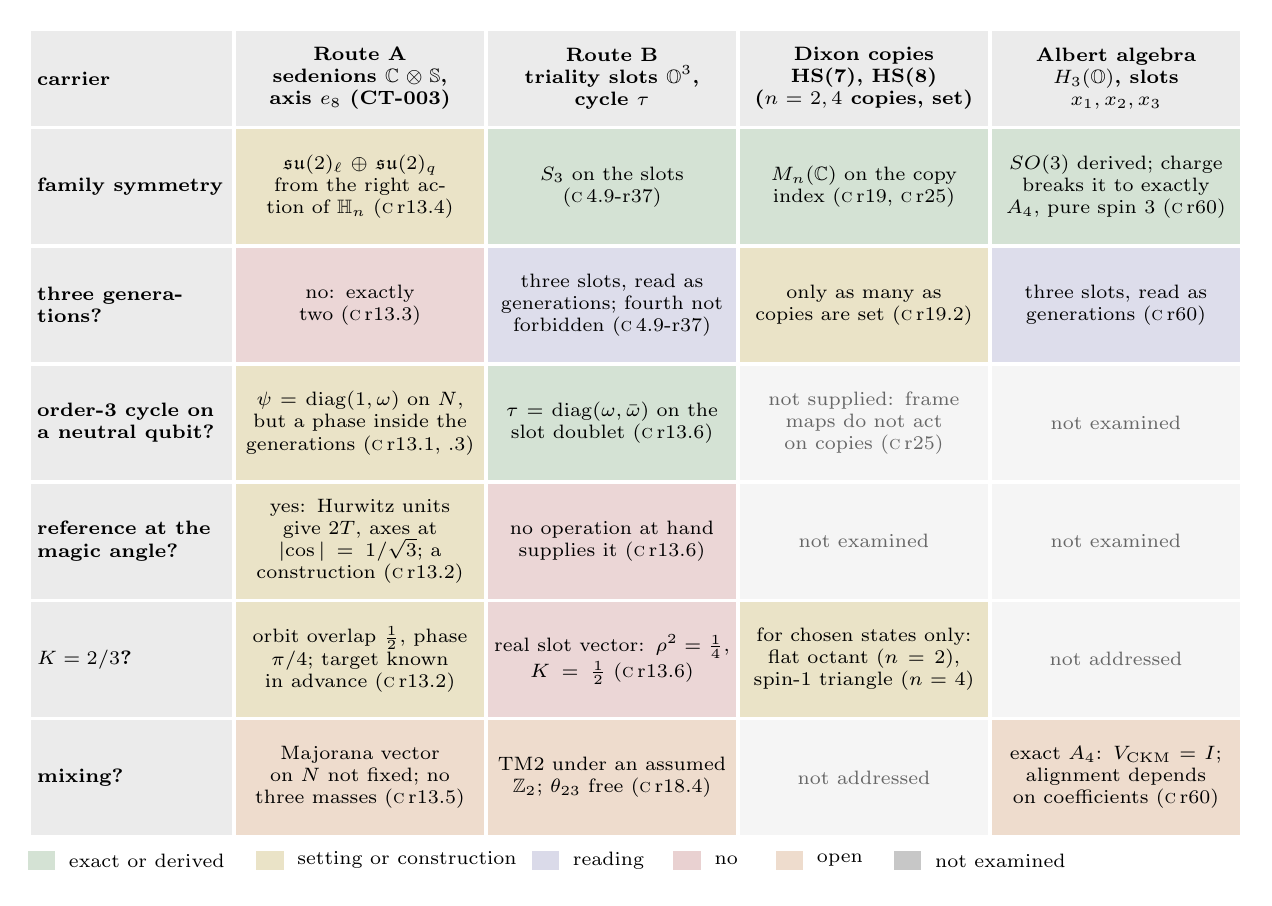
\begin{tikzpicture}[x=1cm,y=1cm,
  cell/.style={draw=white,line width=1.2pt,minimum width=3.2cm,minimum height=1.5cm,text width=3.0cm,
               align=center,font=\scriptsize,inner sep=2pt,anchor=north west},
  head/.style={cell,font=\scriptsize\bfseries,fill=black!8},
  rowh/.style={cell,minimum width=2.6cm,text width=2.4cm,align=left,font=\scriptsize\bfseries,fill=black!8},
  est/.style={cell,fill=st-est!22},
  cond/.style={cell,fill=st-cond!22},
  read/.style={cell,fill=st-read!20},
  ref/.style={cell,fill=st-ref!20},
  open/.style={cell,fill=st-open!22},
  na/.style={cell,fill=black!4,text=black!60}]
\def\cw{3.2}\def\rh{1.5}\def\hx{2.6}\def\hh{1.25}
\newcommand{\C}[4]{\node[#3] at ({\hx+(#1)*\cw},{-\hh-(#2-1)*\rh}) {#4};}
\newcommand{\Hd}[2]{\node[head,minimum height=\hh cm] at ({\hx+(#1)*\cw},0) {#2};}
\newcommand{\Rw}[2]{\node[rowh] at (0,{-\hh-(#1-1)*\rh}) {#2};}
% header row
\node[rowh,minimum height=\hh cm] at (0,0) {carrier};
\Hd{0}{Route A\\ sedenions $\mathbb C\otimes\mathbb S$,\\ axis $e_8$ (CT-003)}
\Hd{1}{Route B\\ triality slots $\mathbb O^3$,\\ cycle $\tau$}
\Hd{2}{Dixon copies\\ HS(7), HS(8)\\ ($n=2,4$ copies, set)}
\Hd{3}{Albert algebra\\ $H_3(\mathbb O)$, slots\\ $x_1,x_2,x_3$}

% row 1: family symmetry
\Rw{1}{family symmetry}
\C{0}{1}{cond}{$\mathfrak{su}(2)_\ell\oplus\mathfrak{su}(2)_q$ from the right action of $\mathbb H_n$ (\rnd{r13}.4)}
\C{1}{1}{est}{$S_3$ on the slots (\rndold{r37})}
\C{2}{1}{est}{$M_n(\mathbb C)$ on the copy index (\rnd{r19}, \rnd{r25})}
\C{3}{1}{est}{$SO(3)$ derived; charge breaks it to exactly $A_4$, pure spin 3 (\rnd{r60})}
% row 2: three generations
\Rw{2}{three generations?}
\C{0}{2}{ref}{no: exactly two (\rnd{r13}.3)}
\C{1}{2}{read}{three slots, read as generations; fourth not forbidden (\rndold{r37})}
\C{2}{2}{cond}{only as many as copies are set (\rnd{r19}.2)}
\C{3}{2}{read}{three slots, read as generations (\rnd{r60})}
% row 3: cycle on a neutral qubit
\Rw{3}{order-3 cycle on a neutral qubit?}
\C{0}{3}{cond}{$\psi=\mathrm{diag}(1,\omega)$ on $N$, but a phase inside the generations (\rnd{r13}.1, .3)}
\C{1}{3}{est}{$\tau=\mathrm{diag}(\omega,\bar\omega)$ on the slot doublet (\rnd{r13}.6)}
\C{2}{3}{na}{not supplied: frame maps do not act on copies (\rnd{r25})}
\C{3}{3}{na}{not examined}
% row 4: magic angle
\Rw{4}{reference at the magic angle?}
\C{0}{4}{cond}{yes: Hurwitz units give $2T$, axes at $|\!\cos|=1/\sqrt3$; a construction (\rnd{r13}.2)}
\C{1}{4}{ref}{no operation at hand supplies it (\rnd{r13}.6)}
\C{2}{4}{na}{not examined}
\C{3}{4}{na}{not examined}
% row 5: K = 2/3
\Rw{5}{$K=2/3$?}
\C{0}{5}{cond}{orbit overlap $\tfrac12$, phase $\pi/4$; target known in advance (\rnd{r13}.2)}
\C{1}{5}{ref}{real slot vector: $\rho^2=\tfrac14$, $K=\tfrac12$ (\rnd{r13}.6)}
\C{2}{5}{cond}{for chosen states only: flat octant ($n=2$), spin-1 triangle ($n=4$)}
\C{3}{5}{na}{not addressed}
% row 6: mixing
\Rw{6}{mixing?}
\C{0}{6}{open}{Majorana vector on $N$ not fixed; no three masses (\rnd{r13}.5)}
\C{1}{6}{open}{TM2 under an assumed $\mathbb Z_2$; $\theta_{23}$ free (\rnd{r18}.4)}
\C{2}{6}{na}{not addressed}
\C{3}{6}{open}{exact $A_4$: $V_{\rm CKM}=I$; alignment depends on coefficients (\rnd{r60})}
% legend
\begin{scope}[yshift=-10.7cm,font=\scriptsize]
\foreach \c/\t/\x in {st-est/{exact or derived}/0,st-cond/{setting or construction}/2.9,st-read/reading/6.4,st-ref/no/8.2,st-open/open/9.5,black/{not examined}/11.0}{
  \fill[\c!22] (\x,0) rectangle ++(0.35,0.25);
  \node[anchor=west] at (\x+0.4,0.125) {\t};}
\end{scope}
\end{tikzpicture}
\caption{Four candidate carriers for a generation index, and what each delivers. Cell colours give the status in the
Companion: green exact or derived, yellow under a named setting or a construction whose target was known, purple a
reading, red a negative answer, orange open, grey not examined. No column delivers three generations, an order-three cycle,
the magic-angle reference, $K=2/3$ and a mixing pattern at once. Route~A and route~B are complementary
(\rnd{r13}.6): the quaternion group needs a doublet made of two slots, the slot cycle needs three slots.}
\label{fig:B-routes}
\end{figure}


\subsection{The Albert algebra and \texorpdfstring{$A_4$}{A4}}
\label{sec:B-albert}

Round \rnd{r60} takes the carrier $H_3(\mathbb O)$ of Hermitian $3\times3$ octonion matrices with the Jordan product
$X\circ Y=\tfrac12(XY+YX)$. Its three off-diagonal octonions are the slots, $\operatorname{Aut}=F_4\supset\mathrm{Spin}(8)$
carries triality, colour is the diagonal $SU(3)_c$, and charge is the slot-wise $C=L_{e_7}$. Reading the slots as
generations is a reading; the following statements are algebra (Wolfram exact, scripts \texttt{k275}--\texttt{k277}).

\begin{proposition}[\rnd{r60}.1, .3, .4]\label{prop:B-albert}
\begin{enumerate}
\item[(a)] The commutant of $G_2$ in $F_4$ is the real $SO(3)$ acting by $X\mapsto RXR^{\mathsf T}$. Under it every colour
triplet is spin $1$; the colour singlets decompose as $1\oplus3\oplus5$.
\item[(b)] Charge breaks this family $SO(3)$ to exactly $A_4$, with the slots in its three-dimensional irreducible
representation.
\item[(c)] On the colour triplets every $A_4$-invariant operator is $SO(3)$-invariant. Hence, with exact $A_4$, quark masses
are degenerate and $V_{\rm CKM}=I$.
\item[(d)] For a flavon $v$ in the $e_7$ parts of the slots, $Y=C\,X(v)$ is real symmetric with zero diagonal and entries
$-v_k$, and its cubic Albert norm is $N(Y)=\det Y=-2\,v_1v_2v_3$, with $\operatorname{Tr}Y=0$, $\operatorname{Tr}Y^2=2|v|^2$.
\end{enumerate}
\end{proposition}

\begin{proof}[Proof sketch]
(b) Of the 24 signed permutations of determinant $+1$, exactly the 12 with even slot permutation commute with charge; the
odd ones exchange $x_{ij}$ with $\bar x_{ij}$, and conjugation turns $L_{e_7}$ into $-R_{e_7}$. The residual Lie algebra is
zero, and every finite subgroup of $SO(3)$ containing $A_4$ is $A_4$, $S_4$ or $A_5$; an icosahedral rotation breaks.
(c) Spin $1\otimes1$ contains $l=0,1,2$ only, and $A_4$ has no invariant at $l=1$ or $l=2$. Since $C$ is $A_4$-invariant, any
$SO(3)$-equivariant construction from $C$ stays $SO(3)$-invariant on the triplets. (d) A real symmetric matrix with zero
diagonal and off-diagonal entries $a,b,c$ has determinant $2abc$.
\end{proof}

The $A_4$ that earlier rounds set by hand as a slot symmetry is here the remnant of a derived family symmetry. The test
H127 asked which spin carries the breaking. Stage~A was \textbf{confirmed}: the charge part
$A_0=P_sCP_s$ lies entirely in the spin-3 component ($w_3=1$, $w_{l\neq3}=0$), a single tensor of type $xyz$, the object that
$A_4$ flavon models introduce by hand. Stage~B (a leak into the quarks at some order) was \Refuted{} by its wording, and by
(c) it is empty for every $SO(3)$-compatible coupling. Quark mixing therefore requires that $A_4$ itself breaks.

The vacuum alignment is not fixed. A potential built only from $Y$ depends on $|v|^2$ and $v_1v_2v_3$, and its minimum is of
type $(1,1,1)$ with residual $\mathbb Z_3$; with the mixed quartic invariants the potential is the general $A_4$ potential,
and the minimum depends on the coefficient of $\sum_iv_i^4$: the two sample values computed give type $(1,1,1)$ and type $(1,0,0)$ (residual $\mathbb Z_2$). This is
the known $A_4$ phase diagram, and the coefficients are free. No blind test of the alignment is possible at present
(\rnd{r60}.5). Set remain the slots as generations, the flavon placement, the coefficients, every mass and every scale.

\subsection{A relative CP sign between leptons and quarks}
\label{sec:B-cp}

On route A the right multiplications obey the quaternion relations with opposite orientation on the neutral and on the
coloured part (\rnd{r13}.4), a consequence of the non-associativity of the sedenion product. In terms of the neutral family
$\mathfrak{su}(2)$ (\rnd{r14}.4, under CT-003):
\begin{equation}
 [R_{e_7},R_{e_8}]=-2R_{e_{15}}\ \text{on the lepton block},\qquad [R_{e_7},R_{e_8}]=+2R_{e_{15}}\ \text{on the coloured block}.
 \label{eq:B-cp}
\end{equation}
For three projectors onto the $+1$ eigenstates of generators with $[J_x,J_y]=isJ_z$, $s=\pm1$, the Bargmann invariant is
$\operatorname{tr}(P_xP_yP_z)=\tfrac14+\tfrac{is}{4}$. Relative to the Lorentz spin (left action of $\mathbb H$, invariant
$\tfrac14+\tfrac i4$) the lepton doublet is the complex-conjugate one: $\tfrac14-\tfrac i4$ on leptons against
$\tfrac14+\tfrac i4$ on quarks, in all $24+24$ assignments of full rank. This is H125 stage~A, \textbf{confirmed} but
\emph{not blind} (\rnd{r59}.6). The relative sign survives $i\mapsto-i$, which conjugates both sectors at once; it is the
first sign in this series that is not a convention.

Stage~B is a prediction against future data. Under the setting S1 (CP arises in both sectors in the same way from the
family structure) one has $\operatorname{sign}J_{\rm PMNS}=-\operatorname{sign}J_{\rm CKM}$, that is
$\sin\delta_{\rm PMNS}<0$. It is decided by the first analysis that fixes the sign at $\ge3\sigma$, with deadline
31~December~2035; the prior probability is $\tfrac12$, and a confirmation would mainly support S1. \Open.

The absolute handedness is different. Every attempt to fix it in \rnd{r59}.1--.4 set it somewhere, and the open choice
ended at the choice of $i$, which over $\mathbb C$ is a convention (\rnd{r59}.4, \rnd{r59}.15). The orientation of the
Koide octant in Section~\ref{sec:B-koide-orientation} is of the same kind.

\paragraph{Summary of the section.}
Under named choices one generation with its charges, chirality and anomaly freedom follows from $\mathbb C\otimes\mathbb H
\otimes\mathbb O$; this is a consistency result in a known line of work. The number of generations is not derived: one
generation admits no generation qubit, route~A gives two generations, route~B gives three slots without the Koide
reference, copies give whatever number is set, and the Albert algebra gives a derived family $SO(3)$ broken to $A_4$ with
the slots read as generations. Masses, mixing angles and scales are not derived anywhere in this section. OP3 and OP4 remain
\Open.

% Section 5 (group B): Koide as geometry. Sources: Companion thm:koide-triolic (status), rounds v4.10.0-r12, r13.2, r14,
% r15, r16, r17, r19, r25, r28, r30, r31 (H118), r59; tests from wiki/Vorhersagen-und-Tests.md.
\section{Koide as geometry, not as derivation}
\label{sec:B-koide}

For three non-negative mass roots $x_k=\sqrt{m_k}$ the Koide ratio is
\begin{equation}
 K=\frac{\sum_k x_k^2}{\bigl(\sum_k x_k\bigr)^2}\in\bigl[\tfrac13,1\bigr].
 \label{eq:B-koide}
\end{equation}
For the charged-lepton pole masses $K=\tfrac23$ holds to better than $0.005\,\%$ \cite{Koide1983}. In the Companion this is an
empirical fact whose derivation is \Open{} (\cite{QSC}, \texttt{thm:koide-triolic}; \rnd{r12}.1). This section collects
what the construction says about it. The result is geometric and largely \Established: $K=\tfrac23$ is equivalent to a
statement about three states with overlap $\tfrac12$, the boundary of the admissible family is the octant of a qubit, and the
bend away from the boundary has an exact form. None of it derives $K=\tfrac23$.

We state the point plainly, because it is easy to miss in a calculation. \emph{The overlap $\tfrac12$ is an input.} Every
construction below that produces $K=\tfrac23$ does so because the overlap $\tfrac12$, or a parameter condition equivalent to
it, was put in. Inserting such a condition (the radius $r=\sqrt2$ of the Brannen form, equal weights of two couplings, or any
fixed ratio of parameters chosen to give $\rho^2=\tfrac12$) presupposes the Koide relation; it does not explain it.

\subsection{The Gram reading}
\label{sec:B-gram}

Let $v_1,v_2,v_3$ be unit vectors with Gram matrix $G_{ij}=\langle v_i,v_j\rangle$, and read the mass roots as the eigenvalues
of $G$ up to a common scale, $x_k=s\,\lambda_k(G)$. This root law is itself a setting.

\begin{proposition}[\rnd{r12}.2]\label{prop:B-gram}
Put $\rho^2=\tfrac13\sum_{i<j}|\langle v_i,v_j\rangle|^2$. Then
\begin{equation}
 K=\frac{\operatorname{Tr}G^2}{(\operatorname{Tr}G)^2}=\frac{1+2\rho^2}{3},\qquad
 K=\tfrac23\iff\rho^2=\tfrac12 .
 \label{eq:B-K-rho}
\end{equation}
\end{proposition}

\begin{proof}
$\operatorname{Tr}G=3$ and $\operatorname{Tr}G^2=\sum_{ij}|G_{ij}|^2=3+2\sum_{i<j}|G_{ij}|^2=3+6\rho^2$. Since $G$ is Hermitian
and positive semidefinite, $\sum_k\lambda_k^2=\operatorname{Tr}G^2$ and $\sum_k\lambda_k=\operatorname{Tr}G$.
\end{proof}

Thus $K=\tfrac23$ is a mean squared overlap of $\tfrac12$: three readout states pairwise half-way, in Fubini--Study distance
$\pi/4$, between equal and orthogonal. Equivalent forms are on record: the angle $\pi/4$ between the root vector and
$(1,1,1)$ \cite{Foot1994}, and the Brannen parametrisation $x_k=a[1+r\cos(\theta+2\pi k/3)]$ with $K=\tfrac13+r^2/6$, so
$K=\tfrac23\iff r=\sqrt2$ \cite{Brannen2010}. The remark that ``$\tfrac23$ is everywhere'' in the construction is a list
of coincidences and not a result (\rnd{r12}.2).

\subsection{The bent octant}
\label{sec:B-bent}

Fix the three pairwise overlaps at $|G_{ij}|^2=\tfrac12$. Rephasing $v_j\mapsto e^{i\alpha_j}v_j$ changes $G_{ij}$ by
$e^{i(\alpha_j-\alpha_i)}$ and leaves the Bargmann invariant $G_{12}G_{23}G_{31}=e^{i\varphi}/(2\sqrt2)$ unchanged, so the
triple is characterised by one phase $\varphi$. A convenient representative is circulant,
\begin{equation}
 G(\varphi)=I_3+\tfrac1{\sqrt2}\bigl(e^{i\varphi/3}U+e^{-i\varphi/3}U^*\bigr),\qquad U(z_1,z_2,z_3)=(z_2,z_3,z_1),
 \label{eq:B-circulant}
\end{equation}
with eigenvalues
\begin{equation}
 \lambda_k(\varphi)=1+\sqrt2\cos\Bigl(\frac{\varphi}{3}+\frac{2\pi k}{3}\Bigr),\qquad k=0,1,2,
 \label{eq:B-roots}
\end{equation}
which is the Brannen form at $r=\sqrt2$ with $\theta=\varphi/3$.

\begin{proposition}[Bent axes, \rnd{r14}.5]\label{prop:B-bent}
Three states with pairwise overlap $\tfrac12$ give $K=\tfrac23$ for every Bargmann phase $\varphi$, and
\begin{equation}
 \det G=\tfrac12\bigl(\sqrt2\cos\varphi-1\bigr).
 \label{eq:B-detG}
\end{equation}
In the principal range, $G$ is positive definite for $|\varphi|<\pi/4$ (three positive roots, the states span
$\mathbb C^3$), has rank two at $|\varphi|=\pi/4$ (one root vanishes, the states lie in one qubit), and is not a Gram
matrix for $|\varphi|>\pi/4$.
\end{proposition}

\begin{proof}
$K=\tfrac23$ follows from Proposition~\ref{prop:B-gram}. For a $3\times3$ matrix with unit diagonal,
$\det G=1-\sum_{i<j}|G_{ij}|^2+2\operatorname{Re}(G_{12}G_{23}G_{31})=1-\tfrac32+\tfrac{1}{\sqrt2}\cos\varphi$. All
$2\times2$ principal minors equal $\tfrac12>0$, so by Sylvester's criterion positivity is decided by the sign of $\det G$.
\end{proof}

The formula and its zero at $\varphi=\pi/4$ are checked numerically against the circulant matrix (deviation below
$10^{-15}$, script \texttt{F6\_detG.py}); Figure~\ref{fig:B-detG} shows both.

\paragraph{The flat octant is the boundary.}
For a qubit, $|\langle a|b\rangle|^2=\tfrac12(1+\mathbf n_a\cdot\mathbf n_b)$ with Bloch vectors $\mathbf n$. Overlap $\tfrac12$
therefore means orthogonal Bloch vectors, and three qubit states with pairwise overlap $\tfrac12$ are, up to rotation, the
eigenstates $+x,+y,+z$ of $\sigma_x,\sigma_y,\sigma_z$: the octant. Its geodesic triangle encloses the solid angle $\pi/2$,
and its Bargmann phase is half of it, $\pi/4$. The octant is rigid: on the Bloch sphere a smaller enclosed area with the
same overlaps is impossible, and the states always have rank two. Hence the boundary of the Koide arc,
$\rho^2=\tfrac12$ at $\varphi=\pi/4$, is exactly the octant triple of three spin-$\tfrac12$ states (\rnd{r12}.4(c)),
with roots $\bigl(\tfrac{3+\sqrt3}{2},0,\tfrac{3-\sqrt3}{2}\bigr)$: one mass is zero. \Established.

\paragraph{Bending needs a third dimension.}
Three positive masses require $\varphi<\pi/4$ and hence leave the qubit for $\mathbb C^3$. The charged-lepton root ratios
$1:14.38:58.97$ are reproduced at $\varphi=\tfrac23$ (Brannen's $\delta=\tfrac29$ times three), with $\det G=0.0557$; this
value is fitted, not derived, and the bend $\pi/4-\tfrac23=0.118731$ is the quantity to be explained. One native way to leave the
qubit is spin one (\rnd{r15}.3): three spin-1 coherent states, symmetric about a cycle axis, with pairwise overlap
$\cos^4(a/2)=\tfrac12$ have side angle $\cos a=\sqrt2-1$, axis angle $38.68^\circ$, $K=\tfrac23$ and Bargmann phase
\begin{equation}
 \varphi=3\arccos\bigl(1-\tfrac1{\sqrt2}\bigr)-\pi=0.679042,\qquad \det G=0.0503,
 \label{eq:B-spin1}
\end{equation}
rank three with root ratios $1:16.24:65.93$. Spin-$j$ coherent-state overlaps are the $2j$-th powers of the spin-$\tfrac12$
overlaps, so the Bargmann phase is $j$ times the enclosed solid angle (a standard property \cite{Perelomov1986}, not a Companion
result); the spin-one triangle is smaller than the octant and bends without any extra structure. The remainder to the lepton
phase is $0.012376$, and no native axis was found among 143 candidates fixed beforehand. The direction is not independent: it
follows from the overlap $\tfrac12$ alone. Symmetric constructions on the carrier fix $\varphi$ by their spin
($0.785$, $0.679$, $0.650$, $0.637$ for $j=\tfrac12,1,\tfrac32,2$), and $\tfrac23$ is not among them (\rnd{r28}.2).
Figure~\ref{fig:B-bloch} shows the flat octant and the spin-one triangle.

\begin{figure}[t]
\centering
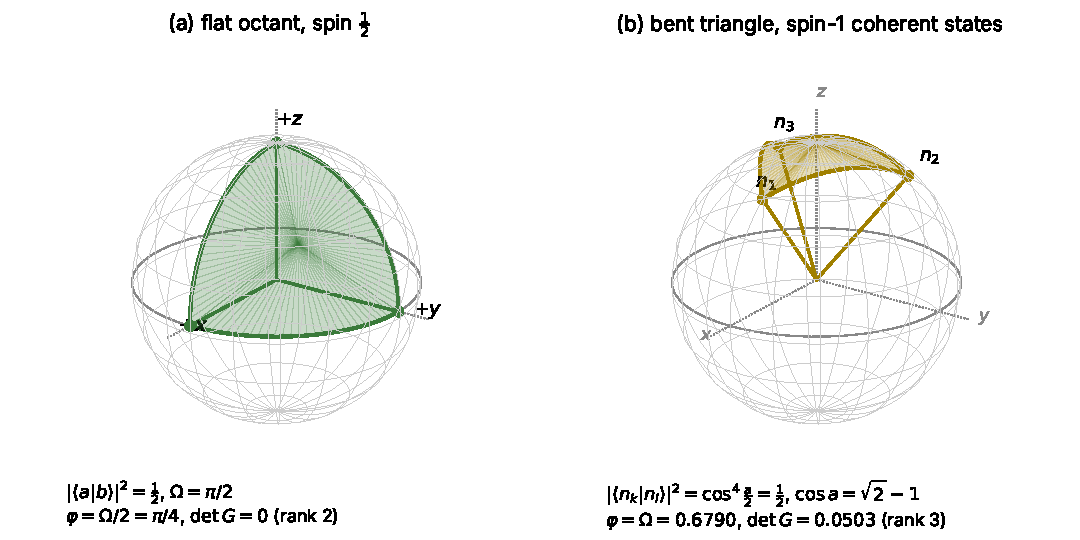
\includegraphics[width=\textwidth]{figures/F5-koide-bloch.pdf}
\caption{Flat against bent. (a) Three spin-$\tfrac12$ states with pairwise overlap $\tfrac12$ have orthogonal Bloch vectors:
the octant, solid angle $\pi/2$, Bargmann phase $\pi/4$, $\det G=0$, one mass zero (\rnd{r12}.4(c), \rnd{r14}.5).
(b) Directions of three spin-1 coherent states with the same overlap: side angle $\cos a=\sqrt2-1$, solid angle and phase
$0.679042$, $\det G=0.0503$, three positive masses (\rnd{r15}.3). Both panels have $K=\tfrac23$ because the overlap
$\tfrac12$ is put in. Status: exact geometry; the physical readout is a setting. Numbers from \texttt{scripts/F5\_koide\_bloch.py}.}
\label{fig:B-bloch}
\end{figure}

\begin{figure}[t]
\centering
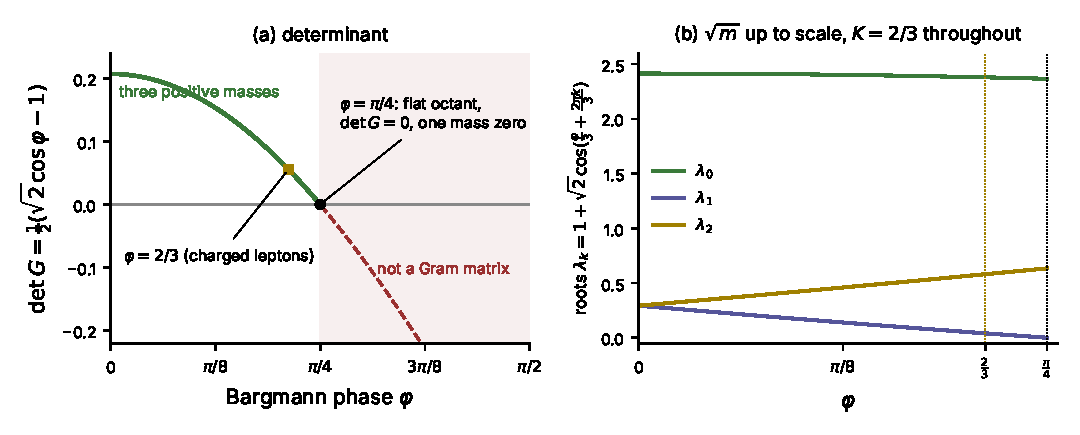
\includegraphics[width=\textwidth]{figures/F6-detG.pdf}
\caption{(a) $\det G=\tfrac12(\sqrt2\cos\varphi-1)$ for three states with pairwise overlap $\tfrac12$. It vanishes exactly at
$\varphi=\pi/4$ (flat octant, one massless state) and is negative beyond, where no Gram matrix exists. The square marks
$\varphi=\tfrac23$, where the circulant roots reproduce the charged-lepton ratios (a fit). (b) The three roots
\eqref{eq:B-roots}; $K=\tfrac23$ on the whole interval. Status: exact (\rnd{r14}.5); the value of $\varphi$ is not derived.
Numbers from \texttt{scripts/F6\_detG.py}.}
\label{fig:B-detG}
\end{figure}

\paragraph{A guarded core as reading.}
The Companion offers one reading of the bend, recorded as a \Reading{} (\rnd{r14}.6). Read a flux-free cap of solid angle
$\Omega$ on the generation sphere (the guarded core of the orbit scan) as removed from the octant. On a sphere with $n$ caps
there are $n-1$ free Aharonov--Bohm holonomies; exactly one core is the only number that bends without a free parameter. If
the displaced flux sits at the antipode, which the antilinear reflector with $\Theta^2=-1$ suggests, the phase is
$\varphi=\pi/4-\Omega/2$. With $\Omega=\gamma_M=0.237533$, the matter-frame value of Section~\ref{sec:beta}, this is the relation of test
H102, $m_\tau=1777.134$\,MeV (exact Koide gives $1776.969$\,MeV). H102 rests on the placeholders CT-001 and CT-002; it is
\Open{} until the first PDG edition after 13~November 2026 (at the latest end of 2028), and against PDG 2024
($1776.93\pm0.09$\,MeV, unchanged in PDG 2026) it stands at $+2.3\sigma$ (\rnd{r28}.3). The core size is thereby OP1 again
(\rnd{r14}.7, \rnd{r28}.2).

\subsection{Why three, and why one half: complementarity}
\label{sec:B-complementarity}

The octant consists of one eigenstate each of $\sigma_x$, $\sigma_y$, $\sigma_z$, one state from each of the three mutually
unbiased bases of a qubit. This generalises.

\begin{proposition}[\rnd{r15}.4]\label{prop:B-mub}
In dimension $d$ take one state from each of $d+1$ mutually unbiased bases. The $N=d+1$ states have
\begin{equation}
 K=\frac{\operatorname{Tr}G^2}{(\operatorname{Tr}G)^2}=\frac{2}{d+1}=\frac2N ,
 \label{eq:B-mub}
\end{equation}
and their Gram matrix has rank at most $d<N$. Only $d=2$ gives three states, with $K=\tfrac23$.
\end{proposition}

\begin{proof}
States from different unbiased bases have overlap $1/d$. Hence $\operatorname{Tr}G=N$ and
$\operatorname{Tr}G^2=N+N(N-1)/d=2N$, because $N-1=d$. The rank bound holds because the states lie in $\mathbb C^d$.
\end{proof}

Read this way, ``three generations'' and ``Koide $\tfrac23$'' are one statement, $K=2/N$ at $N=3$. Two principles are assumed:
one state per complementary basis, and a complete set. \Reading.

\subsection{The octant on a Lorentz-invariant doublet}
\label{sec:B-doublet}

Where could three such states live natively? Round \rnd{r16} places them on the field doublet. With $F_\pm=E\pm iB$ and the
bilinear squares $s_\pm=F_\pm\cdot F_\pm$, a boost acts on $F_+$ by some $M\in SO(3,\mathbb C)$ and on $F_-$ by $\bar M$, so
$s_\pm$ are invariant and
\begin{equation}
 \chi=\bigl(\sqrt{s_+},\sqrt{s_-}\bigr)
 \label{eq:B-chi}
\end{equation}
is a doublet whose Bloch sphere does not depend on the observer. Real fields lie on its equator, self-dual and anti-self-dual
non-null fields at the poles, and plane waves ($s_+=s_-=0$) have no point. The roots carry a sign; a point of $\chi$ is fixed
up to $R$. On $\chi$ the three frame maps of Section~\ref{sec:A-frames} act, up to phase, as
\begin{equation}
 R=\sigma_z,\qquad T=\sigma_x,\qquad J_B=\sigma_y
 \label{eq:B-frame-pauli}
\end{equation}
(checked on 200 real fields, deviation $4\cdot10^{-16}$). Each keeps exactly one of three field signs, $R$ the helicity sign,
$T$ the sign of $\operatorname{Re}s$ (matter against tachyon), $J_B$ the sign of $\operatorname{Im}s$; on the signs they form
the Klein four-group. A matter field ($s=1$), a field of the photon side ($s=i$) and a self-dual field ($E=iB$) give pairwise
overlap $\tfrac12$, $K=\tfrac23$ and Bargmann phase $\pm\pi/4$, and all three rays are unchanged under boosts (\rnd{r16}.3).
The phase needs complex amplitudes: for every octant $\sum_kb_{y,k}^2=1$ in the helicity component, and three states without
helicity component have phase $0$ or $\pi$ (\rnd{r16}.2). The three bases of the doublet, their Stokes-type sphere and the
helicity axis are in the literature \cite{A-Golat2024}; in the Companion's language they are the eigenbases of $T$, $J_B$ and $R$.

\begin{proposition}[Readouts of one object, \rnd{r16}.7]\label{prop:B-readouts}
The eigenrays of $R$, $T$, $J_B$ on $\chi$ are the six poles $\pm x,\pm y,\pm z$. A set of these poles without an
orthogonal pair has at most three elements; there are exactly eight such sets of three, and each is an octant with pairwise
overlap $\tfrac12$, $K=\tfrac23$ and Bargmann phase $\pm\pi/4$.
\end{proposition}

\begin{proof}
Two poles are orthogonal exactly when they are antipodal. A set without an antipodal pair contains at most one pole from each
of the three axes, so at most three elements, and the maximal sets are the $2^3=8$ choices of one sign per axis. Poles from
different axes have orthogonal Bloch vectors and overlap $\tfrac12$; the rest is the octant computation above.
\end{proof}

The reading attached to this is \Reading{} and \emph{not blind}: require (1) that a readout is an eigenstate of a frame map,
(2) that two readouts of one object are not orthogonal, and (3) that all such readouts occur. Then the number three, the overlap
$\tfrac12$ and the phase $\pi/4$ follow together, unique up to frame maps and orientation, and no threefold cycle is needed.
The targets were known and the conditions were stated afterwards; (1), (3), the sign of the phase, the bend and a charged
carrier remain open. The last point is serious: by Proposition~\ref{prop:B-commutant} the generation index cannot sit on the
frame doublet of one generation, so on a charged carrier this reading takes the number of generations as input (\rnd{r19}.2).
The computations on the field doublet stand.

\paragraph{Prior art.}
The octant triple from three mutually unbiased bases, its phase $e^{i\pi/4}$, amplitudes as roots of $z^3=(1+i)/4$, the
charged-lepton form $1+\sqrt2\cos(2g\pi/3+2/9)$ and the neutrino phase $2/9+\pi/12$ appear in Brannen \cite{Brannen2010};
the angle $\pi/4$ is due to Foot \cite{Foot1994}, and $\delta\approx2/9$ is discussed by \.Zenczykowski \cite{Zenczykowski2012}.
The octant, its phase and the shift $\pi/12$ are therefore not results of the Companion. What is specific here is their
placement on the frame maps of the field doublet, restricted by \rnd{r19}.2 (\rnd{r19}.4).

\subsection{The Brannen form as a time cycle}
\label{sec:B-time-cycle}

The doublet also carries a native threefold cycle. For time-harmonic fields the instantaneous invariant decomposes exactly as
\begin{equation}
 s(t)=\bigl(E(t)+iB(t)\bigr)^2=\tfrac14\bigl(s_+e^{-2i\omega t}+2w+\bar s_-e^{2i\omega t}\bigr),\qquad w=F_+\cdot\bar F_-,
 \label{eq:B-st}
\end{equation}
and $w$ is a third Lorentz invariant (\rnd{r16}.8). Translation by one third of the period of $s(t)$ acts on $(s_+,w,\bar s_-)$
as $U=\operatorname{diag}(\bar\omega_3,1,\omega_3)$, $\omega_3=e^{2\pi i/3}$. A state with weights $(p_-,p_0,p_+)$,
$\sum p=1$, has an orbit of three states with circulant Gram matrix and
\begin{equation}
 |\langle\psi|U\psi\rangle|^2=\bigl|p_0+p_-\bar\omega_3+p_+\omega_3\bigr|^2=\tfrac12\Bigl(3\sum_kp_k^2-1\Bigr),
 \label{eq:B-autocorr}
\end{equation}
so Koide is $\sum p^2=\tfrac23$, with $p_k=\sqrt{m_k}/\sum\sqrt m$: the autocorrelation of the invariant after one third of
its period has modulus $1/\sqrt2$ (\rnd{r16}.9). The cycle is native and produces the Brannen form; the weights are Brannen's
parameters in another form. No principle in the inventory fixes $\sum p^2=\tfrac23$, and a search over 24 candidate constants
listed beforehand found no hit. The photon-clock functional of the Companion has the same form, but no window threshold lies at
$\tfrac12$, so the clock does not fix the overlap either (\rnd{r17}.1). Reading the overlap $\tfrac12$ as maximal
uncertainty (a one-bit question with probability $\tfrac12$) is a further \Reading{} with the maximisation assumed
(\rnd{r17}.2). All of this is \Exploration, not blind.

\subsection{The orientation of the octant step}
\label{sec:B-koide-orientation}

The octant fixes the modulus of the phase, not its sign. The loops $x\to y\to z\to x$ and $x\to z\to y\to x$ have the same
endpoints and the same three transition probabilities $\tfrac12$, but ordered overlap products $(1+i)/4$ and its conjugate,
steps of $+\pi/4$ and $-\pi/4$. Three pre-registered tests, all \emph{not blind} because the outcome was fixed analytically
beforehand, locate the open choice (\rnd{r30}.10--.12):
\begin{itemize}
\item H115: on the closed odd generation states $JS=-S$, so the direct compensator gives $CS=0$, rank zero. A real rank-five
halving exists only with an additional phase choice on a complex null line.
\item H116: magnitudes and endpoints do not fix the sign; even a uniform histogram of accumulated phases says nothing, since
both constant step sequences $\pm1$ modulo eight visit all eight phases.
\item H117: in a two-window model, of the 16 mask pairs three give $+\pi/4$, three give $-\pi/4$, nine are blocked and one is
ambiguous; no repair rule decides between the signs.
\end{itemize}

Test H118 then classifies the sign (\rnd{r31}.1). For the eight triples of Proposition~\ref{prop:B-readouts} the Bargmann
phase is exactly
\begin{equation}
 \varphi=\tau\,\varepsilon\,\frac{\pi}{4},
 \label{eq:B-orientation}
\end{equation}
with $\tau=\pm1$ the direction of the loop $R\to T\to J_B$ and $\varepsilon$ the product of the three pole signs.
$R$, $T$, $J_B$ and parity ($E\mapsto-E$, acting as $\sigma_x$) preserve the orientation; time reversal of the complex field
amplitudes ($E\mapsto\bar E$, $B\mapsto-\bar B$) maps $s_\pm\mapsto\bar s_\pm$, acts on $\chi$ as complex conjugation and
reverses it. This is the distinction of Section~\ref{sec:A-frames}: time reversal $z\mapsto\bar z$ is not the tachyon map $z\mapsto iz$. None of
nine candidates listed beforehand selects an orbit natively. H118a (the formula) is confirmed, H118b (a native selection) is
\Refuted. The sign of the octant step is a time orientation of the readout and is not fixed by the Companion. Round
\rnd{r59} followed this handedness further and found it set at every step, ending at the choice of $i$, a convention; only the
relative sign between leptons and quarks of Section~\ref{sec:B-cp} is not a convention.

\subsection{Tests that ground the result}
\label{sec:B-koide-tests}

Table~\ref{tab:B-koide-tests} lists the tests that bear on this section. Two are open predictions. The refuted ones are
listed because they ground a negative result: the Bargmann phase is rigid in the carrier geometry. Copies, entanglement,
frame-dependent readouts and nested normalisations of the carrier states (H106--H111) do not move the phase from the
spin-one value $0.679$ to $\tfrac23$; only a change of the connection on the generation sphere, as in the core reading, escapes
this rigidity (\rnd{r28}.2).

\begin{table}[t]
\centering\small
\begin{tabularx}{\textwidth}{@{}l>{\raggedright\arraybackslash}X>{\raggedright\arraybackslash}p{0.27\textwidth}@{}}
\toprule
test & statement & status\\
\midrule
H99 & equal overlap $\rho^2=\tfrac12$ for charged leptons and neutrinos, $\theta_\nu=\theta_e+\pi/12$:
$\Delta m^2_{21}/\Delta m^2_{31}=0.030839$ & compatible, $+1.80\sigma$ (NuFIT 6.1); \emph{not blind} (\rnd{r12}.5)\\
H100 & three values of that ratio fixed for the next NuFIT release & open (\rnd{r12}.5)\\
H101 & lepton mask lifts the electron off the qubit octant & refuted: the form preserves the rank, the electron stays massless\\
H102 & $\varphi_e=\pi/4-\gamma_M/2$ gives $m_\tau=1777.134$\,MeV & open; $+2.3\sigma$ against PDG 2024 (\rnd{r28}.3)\\
H103a & inherited charge fixes the magic-angle reference on $N$ & refuted; gives $K=\tfrac12$ (\rnd{r13}.1)\\
H106--H111 & carrier variants (singlet admixture, nested normalisation, entangled copies, frame-dependent readouts, time octant)
close the residual bend & refuted; no hit (\rnd{r28})\\
H115--H117 & compensator, endpoints or two windows fix the sign of the octant step & as stated above; not blind (\rnd{r30})\\
H118 & a native structure fixes the orientation & formula confirmed, selection refuted (\rnd{r31})\\
\bottomrule
\end{tabularx}
\caption{Tests bearing on the Koide geometry (status from \texttt{wiki/Vorhersagen-und-Tests.md} and the cited rounds).}
\label{tab:B-koide-tests}
\end{table}

\paragraph{Summary of the section.}
\Established: $K=(1+2\rho^2)/3$; three states with overlap $\tfrac12$ give $K=\tfrac23$ for every phase, with
$\det G=\tfrac12(\sqrt2\cos\varphi-1)$; the boundary is the rigid qubit octant with one massless state; $K=2/(d+1)$ for
complete sets of unbiased states; on the invariant doublet $\chi$ the non-orthogonal frame eigenstates are at most three
and form exactly the octants; the sign of the step is a time orientation. \Reading: the complementarity reading, the
readouts of one object, the time cycle and the guarded core. \Open: the overlap $\tfrac12$ itself, the bend to
$\varphi=\tfrac23$ (equivalently the core size, OP1), the orientation, and a charged carrier with three generations. The
Koide relation is described, not derived; OP3 remains open.

% Section 6 (group C): the frame offset beta_sym and the counting rule (OP1)
\section{The frame offset \texorpdfstring{$\bsym$}{beta\_sym} and the counting rule (OP1)}
\label{sec:beta}

The numerical values that the construction offers for OP2--OP5 go back to one dimensionless number, the frame offset $\bsym\approx0.549$.
This section states how the number is defined, what it rests on, and what has been tried to derive it.  The short answer is that the
number is inserted, not derived: it is fixed by the ratio of two values of the Barbero--Immirzi parameter of loop quantum gravity, read as a Lorentz
factor.  Why two frames should use two different horizon counting rules is open problem OP1 \Open.  The structural routes to a frame-dependent
area quantum that the Companion has examined are closed; what remains is a choice.  Since 26 November 2026 the choice has a name and a status:
the author adopted the counting rule as a \emph{postulate} (\rnd{r67}), in the same sense as the exchange symmetry of Section~\ref{sec:B-koide}.
With it the number is computed from one rule with three named parts instead of being taken as the ratio of two literature values
(Section~\ref{sec:beta-postulate}).  The reason for the rule is still missing, and OP1 stays \Open.

\subsection{The number and its algebra}
\label{sec:beta-number}

Let $\gamma_{\mathrm{BI}}$ be the Barbero--Immirzi parameter from the horizon counting with all spins and weight two
(Domaga{\l}a--Lewandowski, Meissner \cite{DomagalaLewandowski2004,Meissner2004}) and $\gamma_{\mathrm{string}}=\ln2/(\pi\sqrt3)$ the value from the
counting with spin $j=\tfrac12$ only (Ashtekar, Baez, Corichi, Krasnov \cite{ABCK1998}).  The name ``string'' is historical; the value is the
ABCK count (\rnd{r24}, Remark~24.3).

\begin{proposition}[symmetric frame; \cite{QSC}, \texttt{thm:symmetric-frame}]
\label{prop:beta-symmetric}
Let $r>1$ and put $\beta:=\sqrt{(r-1)/(r+1)}$ and $\eta:=\operatorname{artanh}\beta$.  Then
\begin{equation}
 \frac{1+\beta^2}{1-\beta^2}=r=\cosh2\eta,\qquad
 \frac{2\beta}{1+\beta^2}=\tanh2\eta .
 \label{eq:beta-gL}
\end{equation}
Two observers at velocities $+\beta$ and $-\beta$ relative to a common frame therefore have mutual Lorentz factor $r$.
\end{proposition}

\begin{proof}
$(1+\beta^2)/(1-\beta^2)=\bigl((r+1)+(r-1)\bigr)/\bigl((r+1)-(r-1)\bigr)=r$.  With $\beta=\tanh\eta$ one has
$(1+\tanh^2\eta)/(1-\tanh^2\eta)=\cosh2\eta$ and $2\tanh\eta/(1+\tanh^2\eta)=\tanh2\eta$, the relativistic sum of $\beta$ and $\beta$.
\end{proof}

The algebra is \Established.  The physical content is the insertion
\begin{equation}
 r=\gamma_L:=\frac{\gamma_{\mathrm{BI}}}{\gamma_{\mathrm{string}}}=\frac{0.2375330}{0.1273840}=1.864700,\qquad
 \bsym=0.549406,\qquad \eta=0.6175,
 \label{eq:beta-values}
\end{equation}
which is \Conditional\ on reading a ratio of two values of one gravitational parameter as a Lorentz factor between the real projections of the
matter frame M and the tachyon frame T (\rndold{r61}, Theoremlet~61.1(c)).  (The main body of the Companion uses the rounded input $0.2375$, which gives $\bsym=0.549348$; \rndold{r63}.  From \rnd{r67} on the reference value is $\bsym=0.5494056410$, $\gamma_L=1.8646997646$; no recorded verdict depends on the difference.)  The ratio
$\gamma_L$ is $1/b_M$ in the register of Convention~F and the mutual Lorentz factor of two flux-opposed observers M and $\bar{\mathrm M}$; it is not a
boost between M and T, since a boost preserves $s=(E+iB)^2$ while the map to T reverses $\operatorname{Re}s$ (\rnd{r29}, Remark~29.4, read with $D$; \rnd{r64}.7).  In the
observer reading of the register (\rnd{r29}, Theoremlet~29.5), OP1 asks why M moves with $\bsym=0.5494$ relative to the rest frame of the field.

\subsection{The number as a ratio of two horizon counts}
\label{sec:beta-counting}

A horizon counting rule assigns a weight $g(j)$ to each spin $j\in\{\tfrac12,1,\tfrac32,\dots\}$ of a puncture.  With the area spectrum
$a(j)=\sqrt{j(j+1)}$, the Barbero--Immirzi parameter is the positive root of
\begin{equation}
 \sum_j g(j)\,e^{-2\pi\gamma\,a(j)}=1 .
 \label{eq:beta-counting}
\end{equation}
Table~\ref{tab:beta-rules} lists the three rules that matter here (\rndold{r63}, Theoremlet~63.1, rechecked in \rndold{r68}; the values agree
with Meissner's $0.23753295796592$ to the digits shown).

\begin{table}[ht]
\centering\small
\begin{tabular}{@{}llccc@{}}
\toprule
rule & source & $\gamma$ & $\gamma/\gamma_{\mathrm{string}}$ & $\beta$\\
\midrule
$j=\tfrac12$ only, $g=2$ & ABCK \cite{ABCK1998} & $0.1273840$ & $1$ & $0$\\
all $j$, $g=2$ (U(1)) & DL, Meissner \cite{DomagalaLewandowski2004,Meissner2004} & $0.2375330$ & $1.864700$ & $0.549406$\\
all $j$, $g=2j+1$ (SU(2)) & Ghosh--Mitra; ENP \cite{GhoshMitra2005,EngleNouiPerez2010} & $0.2740669$ & $2.151501$ & $0.604468$\\
\bottomrule
\end{tabular}
\caption{Counting rules and the resulting frame offset.  The lepton window $\beta\in[0.545,0.570]$ of \rndold{r61} contains, of these three, only the U(1)
pair.  Status: values \Established\ (numerical roots); their use as frame rules \Conditional.}
\label{tab:beta-rules}
\end{table}

Two facts weigh against the chosen pair.  First, it is a U(1) counting.  The SU(2)-invariant treatment of the horizon
\cite{EngleNouiPerez2010} is regarded in the literature as better founded; it gives $\gamma\approx0.274$ and $\bsym=0.604$, outside the window.
The data therefore select the counting that the later literature considers less well founded (\rndold{r68}, Correction~68.3).  Second, the
selection was made with the window in view (\rndold{r63} is marked not blind).

One mathematical fact supports the reading as a statement about states rather than about parameters.

\begin{proposition}[uncertainty saturation; \rndold{r63}, Theoremlet~63.2]
\label{prop:beta-saturation}
In the state $|j,m\rangle$ ($\hbar=1$) one has $\Delta J_x\,\Delta J_y=\tfrac12\bigl(j(j+1)-m^2\bigr)\ge\tfrac12|m|$, with equality exactly for
$m=\pm j$.  Hence at every $j$ exactly two states saturate the Robertson bound, and at $j=\tfrac12$ every state does.
\end{proposition}

\begin{proof}
$\langle J_x\rangle=\langle J_y\rangle=0$ and $\langle J_x^2\rangle=\langle J_y^2\rangle=\tfrac12\bigl(j(j+1)-m^2\bigr)$, while the Robertson bound is
$\tfrac12|\langle J_z\rangle|=\tfrac12|m|$.  The difference is $\tfrac12(j-|m|)(j+|m|+1)$, which vanishes iff $|m|=j$.
\end{proof}

The weight two of the M rule thus counts the extremal doublet $|j,\pm j\rangle$ at every $j$; Meissner's counting of labels $\pm m$ matches this
\cite{Meissner2004} (\rndold{r68}).  This is a reinterpretation of the U(1) counting, not part of its derivation \Reading.

\subsection{What depends on the rule}
\label{sec:beta-dependence}

The Companion keeps a list of its assumptions, each with an origin category; one category, ``R'', marks assumptions set after a consequence was known
(\rnd{r08}, Remark~8.2).  Bookkeeping of the four predictions open at that time shows that three of them rest on the same core (\rnd{r08}, Theoremlet~8.3):

\begin{center}\small
\begin{tabular}{@{}lll@{}}
\toprule
prediction & statement & inputs besides the literature values\\
\midrule
H96 & $\Omega_M=\bsym^2=0.30185$ & counting rule per frame, epoch ``today''\\
H15 & $m_W=m_Z\gamma_L/\sqrt{1+\gamma_L^2}$ & counting rule, reading $\cot\theta_W=\gamma_L$\\
H46 & $\sin^2\theta_{23}\in[0.49,0.50]$ & counting rule, neutrino reading, mask, $\varepsilon=\eta$\\
H42 & $\sin^2\theta_{23}\le0.54$ & neutrino reading, mask (independent of $\gamma_L$)\\
\bottomrule
\end{tabular}
\end{center}

If the counting rule fails, H15, H46 and H96 fail together.  With the SU(2) counting one would get $m_W=82.69$\,GeV and $\Omega_M=0.365$
instead of $80.361$\,GeV and $0.302$.  The U(1) rule was selected by the lepton window and the $m_W$ relation was noticed afterwards, so these
agreements are not independent of the selection.  The four predictions form two independent groups, not four; of those listed as open since
(Table~\ref{tab:open-tests}), H9 and H102 use the same number and H112 only the equality of two readouts.  Forming $\gamma_L$ without
a declared map from T to M is frame mixing in the sense of Convention~F: $\gamma_L$ is defined only through the reading it supports
(\rnd{r08}, item~8.3(d)).

\subsection{The special position of the pair (H98) and its limits}
\label{sec:beta-h98}

Test H98 asked how special the chosen pair is (\rnd{r09}, Theoremlet~9.1; pre-registered, \emph{not blind}: all three data values and the
agreement of the chosen pair were known).  The rule space has the spin ranges all $j$, half-integer $j$, integer $j\ge1$, $j=\tfrac12$ only and
$j=1$ only, with weights $2$ and $2j+1$: nine distinct rules and $36$ pairs with $\gamma_M>\gamma_T$.  Three windows were fixed: the lepton window
$\beta\in[0.545,0.570]$; $m_W$ within $2\sigma$ of the PDG 2025 average $80.3692\pm0.0133$\,GeV via $\cot\theta_W=\gamma_L$; and $\Omega_M$ within
$2\sigma$ of DESI DR2 BAO, $0.2975\pm0.0086$ \cite{DESIDR2}, via $\Omega_M=\beta^2$.  Two pairs fall in the lepton window, one in the $m_W$ window,
two in the $\Omega_M$ window, and exactly one in all three: all spins with weight two for M and $j=\tfrac12$ for T, with $\gamma_L=1.864700$,
$m_W=80.3615$\,GeV ($0.6\sigma$) and $\Omega_M=0.3018$ ($0.5\sigma$).  The SU(2) pair misses all three.  Figure~\ref{fig:beta-pairs} shows the
$36$ values.

\begin{figure}[t]
\centering
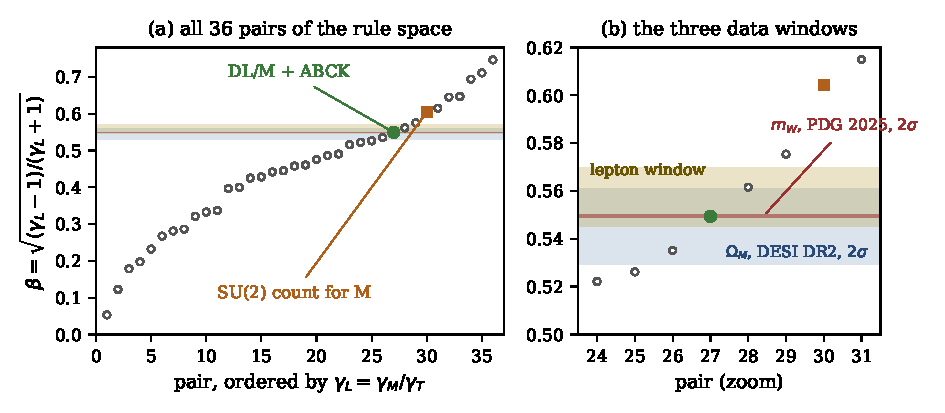
\includegraphics[width=\textwidth]{figures/F7-counting-pairs.pdf}
\caption{Frame offset $\beta=\sqrt{(\gamma_L-1)/(\gamma_L+1)}$ for the $36$ counting-rule pairs of the rule space of H98, ordered by
$\gamma_L=\gamma_M/\gamma_T$.  Filled circle: the pair DL/Meissner for M with ABCK for T; square: the SU(2) count ($g=2j+1$) for M with ABCK for
T.  Bands in (b): lepton window $[0.545,0.570]$, $\Omega_M=\beta^2$ within $2\sigma$ of DESI DR2 BAO, and $m_W$ within $2\sigma$ of PDG 2025
(narrow band).  Recomputed by \texttt{scripts/F7\_counting\_pairs.py} from the rule space of \rnd{r09} (script \texttt{k218}); the values agree with
its stored output.  Status: the confirmation of H98 is \emph{not blind}; with a free area spectrum the position is not unique (H104,
\Refuted), and the hits are compatible with chance once the selection of the pair is counted.}
\label{fig:beta-pairs}
\end{figure}

The weight of this result is limited in three ways.
\begin{enumerate}
\item Only the $m_W$ window selects uniquely, and the $m_W$ relation was itself found afterwards.  The $36$ values of $\gamma_L$ lie between
$1.006$ and $3.51$; the $m_W$ window is about $\pm0.003$ wide in $\gamma_L$, so about $0.08$ pairs would be expected in it.  A chance triple
agreement is of the order of a few per cent (\rnd{r09}).
\item The singular position depends on the fixed spectrum $\sqrt{j(j+1)}$.  With a free area spectrum (23 rules, 253 pairs), a second pair meets
all three windows ($\gamma_L=1.864824$).  The pre-registered test H104 is therefore \Refuted; H98 stays confirmed in its own rule space
(\rnd{r14}, Theoremlet~14.1).  A first run with a faulty solver had reported the opposite; it is disclosed in the Companion.
\item A chance estimate with a procedure fixed before the computation (\rnd{r30}, Remark~30.5) uses 16 targets, eight forms and a $2\sigma$ window.
The pair gives three hits ($\sin^2\theta_{12}$ and $\Omega_m$ by $\beta^2$, $\cot\theta_W$ by $\gamma_L$), the only pair of the 36 with three.  The
probability of at least three hits for a random $\gamma_L$ is $0.018$ to $0.023$; over 36 pairs the expected number is $0.64$ to $0.81$.  While the pair
is chosen rather than derived, the hits are compatible with chance.  The two targets near $0.30$ are strongly correlated, so two of the three hits
are nearly one.
\end{enumerate}

\subsection{Attempts to derive the assignment}
\label{sec:beta-attempts}

All attempts below are explorations \Exploration; their targets were known.

\paragraph{Energy and Unruh statistics.}
A principle was proposed in \rnd{r09} (Remark~9.2): a frame counts the states that saturate the uncertainty bound (P1) and are compatible with
its energy condition (P2), where T, as a tachyon relaxing to its floor (\rndold{r63}, Theoremlet~63.3), reaches only the smallest excitation.  P2 does
not survive.  By the local first law of isolated horizons \cite{FroddenGhoshPerez2013}, an observer at proper distance $\ell$ assigns a puncture of
area $8\pi\gamma a(j)$ ($\ell_P=1$) the energy $E_j=\gamma a(j)/\ell$ and has Unruh temperature $T_U=1/(2\pi\ell)$, so
\begin{equation}
 E_j/T_U=2\pi\gamma\,a(j),
 \label{eq:beta-unruh}
\end{equation}
independent of $\ell$.  Equation~\eqref{eq:beta-counting} is this Boltzmann statistics, and all static observers count alike (\rnd{r10},
Theoremlet~10.1).  The tachyon map commutes with the boost and fixes the vacuum, so an observer in T sees the same KMS state (Theoremlet~10.2).  The
tachyon floor is a property of a particle, not of the state seen at the horizon.

\begin{proposition}[the rule as an area quantum; \rnd{r10}, Theoremlet~10.3]
\label{prop:beta-area}
If M and T see the same statistics, the same geometry and both satisfy $S=A/4$, the assignment of counting rules is equivalent to a
frame-dependent Barbero--Immirzi parameter, $\gamma_M=\gamma_{\mathrm{BI}}$, $\gamma_T=\gamma_{\mathrm{string}}$: the smallest area quantum is smaller
by the factor $\gamma_L$ in T than in M, while the classical area and $G$ are the same.
\end{proposition}

This is an equivalence under stated assumptions \Conditional, not a reason.  The counting rule is from here on an assumption about a
frame-dependent area quantum.

\paragraph{Group theory of the readout.}
Assume (A) that the frame maps act on a puncture of spin $j$ through the same $SU(2)$ as on the field doublet $\chi$, i.e.\ as $e^{-i\pi J_k}$ about
three orthogonal axes.  Then they act irreducibly only for $j=\tfrac12$ (for half-integer $j$ they anticommute and the space splits into copies of
the doublet; for integer $j$ they commute), while the extremal doublet $|j,\pm j\rangle$ is invariant for every $j$.  The rules ``T counts punctures
on which the frame maps act irreducibly'' and ``M counts the invariant extremal doublet'' reproduce exactly the H98 pair (\rnd{r17},
Theoremlet~17.3; checked for $j\le20$).  In a strand picture (a spin-$j$ edge as a symmetrised bundle of $2j$ strands) bosonic strands give all $j$ and
fermionic strands only $j=\tfrac12$ (Theoremlet~17.5), but nothing in the frame or port structure distinguishes the statistics of strands
(\rnd{r24}, Theoremlet~24.1).  What remains is a reading \Reading: T counts crossings of the horizon, one crossing carrying one strand
(\rnd{r24}, Remark~24.4).  It replaces a placeholder (``T = string sector'') by a statement that refers to passages of the Companion (a narrative theorem and a typing), but it derives nothing.

\paragraph{Where the weakest point is.}
Every route to the assignment needs four parts: the area spectrum $\propto\sqrt{j(j+1)}$ (K0, from the literature), weight two for M (K1), all spins
for M (K2) and $j=\tfrac12$ only for T (K3).  Across six routes K0 is always set, K1 has partial supports, K2 none, and K3 only under (A) or explicit
placeholders (\rnd{r30}, Remark~30.4).  Of five reasons collected for the T rule none is free of the data (\rnd{r30}, Remark~30.3).  The rule of T
is a choice.

\paragraph{One number as a dimension.}
In units of the T quantum, equation~\eqref{eq:beta-counting} reads $\sum_j g(j)\,r_j^{D}=1$ with $r_j=2^{-a(j)/a(1/2)}$ and $D=\gamma/\gamma_T$: a
Moran equation of a self-similar set with $g(j)$ copies at scale $r_j$.  Then $D_T=1$, $D_M=\gamma_L=1.8647$ and $D_{\mathrm{SU(2)}}=2.1515$; the M set
fits in the plane and the SU(2) set cannot ($\sum(2j+1)r_j^2=1.199>1$) (\rnd{r29}, Theoremlet~29.3).  Reading the M rule as the richest such structure that fits on a surface is a reading stated afterwards.  A related exact statement: the weight two requires that the maps of $|j,+j\rangle$ and $|j,-j\rangle$
are distinct; if they coincide, or only one is admitted, the M rule falls to $\gamma_1=0.161586$ (\rnd{r53}, Theoremlet~53.2).  Weight two thus
asks for a readout that distinguishes the two orientations of a puncture without selecting one.

\subsection{Structural no-go results for a frame-dependent area quantum}
\label{sec:beta-nogo}

Proposition~\ref{prop:beta-area} asks for a map between frames that changes the area quantum by $\gamma_L$ at fixed $G$.  Three candidates have
been checked; none carries.

\paragraph{Unitary boosts.}
Rovelli and Speziale \cite{RovelliSpeziale2003} show that a boosted observer measures an area operator that does not commute with the original one;
if the boost acts unitarily, both have the same spectrum and the same smallest area, and only the distribution of eigenvalues changes.  Since M
and $\bar{\mathrm M}$ are related by a genuine boost, and the duality part $J_B$ leaves the geometry fixed, no decomposition of the frame map into
boost and duality yields a frame-dependent area quantum while the boost acts unitarily.  The assignment is compatible with standard loop quantum
gravity only if the map $\mathrm M\to\mathrm T$ is not unitary, the $J_B$ image with imaginary rapidity $i\pi/2$ being the only candidate, or if
$\gamma_T$ is read as a mean and not as an eigenvalue parameter, which is not a counting rule (\rnd{r30}, Remark~30.1).  A boost along the horizon normal prefers extremal states but does not select them (Remark~30.2).

\paragraph{Holst term and duality rotations.}
Write the gravitational Lagrangian of the action W1 with a Holst term \cite{Holst1996} as $L=A\langle\star\Sigma,R\rangle+B\langle\Sigma,R\rangle$
with $A=-1/(2\kappa)$ and $B/A=1/\gamma$.

\begin{proposition}[\rnd{r31}, Theoremlets~31.3 and 31.4]
\label{prop:beta-holst}
\textup{(a)} Real boosts, rotations and the complex boost with rapidity $\eta+i\pi/2$ leave $L$ invariant and do not change $\gamma$.
\textup{(b)} A duality rotation of the curvature, $R\mapsto\cos\theta\,R+\sin\theta\star R$, maps $(A,B)\mapsto(A\cos\theta+B\sin\theta,\;B\cos\theta-A\sin\theta)$,
hence $\arctan\gamma'=\arctan\gamma+\theta$.  \textup{(c)} Every sequence of such rotations preserves $A^2+B^2$.  Since the area quantum is
proportional to $\kappa\gamma=-1/(2B)$, for real results
\begin{equation}
 \frac{a'}{a}=\pm\sqrt{\frac{1+\gamma'^2}{1+\gamma^2}} ,
 \label{eq:beta-holst}
\end{equation}
so $\gamma_M\mapsto\gamma_T$ changes the area quantum by $\pm0.981$, not by the factor $\gamma_T/\gamma_M=0.536$ required at equal Newton constant.
\end{proposition}

\begin{proof}
(b) The pair $(A,B)$ is rotated by $-\theta$, and $\gamma'=A'/B'=(\gamma+\tan\theta)/(1-\gamma\tan\theta)=\tan(\arctan\gamma+\theta)$.  (c) Rotations
preserve the Euclidean norm of $(A,B)$.  With $A=\gamma B$,
\[
 A^2+B^2=B^2(1+\gamma^2)\quad\Longrightarrow\quad \frac{B}{B'}=\pm\sqrt{\frac{1+\gamma'^2}{1+\gamma^2}},
\]
and $\sqrt{(1+0.127384^2)/(1+0.237533^2)}=0.981$.  Part (a) and the absence of a distinguished angle ($\theta^*=-0.1065$) are checked in Wolfram
Language in the Companion.
\end{proof}

The only place in W1 plus Holst where a frame-dependent $\gamma$ can arise is a duality rotation of the curvature, which is not a symmetry of the
action; and it cannot produce $\gamma_L$ at equal $G$ by any path.  Part (c) was found afterwards; its algebra is elementary
\Established\ (within this action).

\paragraph{The non-unitary frame map $J_B$.}
$J_B$, conjugation with $\exp(i\tfrac\pi2K_x)$, is an automorphism of the Lorentz algebra, and conjugation by any invertible operator, unitary or not,
keeps every spectrum.  Reading the area in T through the transformed simplicity condition $K=\gamma L$ gives $\Gamma'=\operatorname{diag}(\gamma,-1/\gamma,-1/\gamma)$:
$\gamma$ along the M--T axis, $-1/\gamma$ across it.  At $\gamma_M$ this is $0.2375$ and $-4.2099$, matching neither $\gamma_T$ nor $\gamma_L$; the
pre-registered H121c is \Refuted\ (\rnd{r52}).  In the finite representations checked the complex boost is even unitary; questions of domain in
the infinite-dimensional unitary representations remain open.

With these three results the last structural candidate for a frame-dependent area quantum named in the Companion does not carry.  OP1 rests on the
assignment of the counting rules itself.

\subsection{A temporally ordered octant readout (H123)}
\label{sec:beta-h123}

Weight two asks for a readout that separates the two orientations of a puncture without selecting one.  The octant of Section~\ref{sec:B-koide} offers a candidate:
three readout windows in the order $R\to T\to J_B$ ($\tau=+1$) or reversed, on the extremal states of spin $j$ along $z$, $x$, $y$, with pole-sign
product $\varepsilon$ (\rnd{r58}; pre-registered, H123a--c not blind).

\begin{proposition}[\rnd{r58}, Theoremlets~58.1 and 58.2]
\label{prop:beta-octant}
The Bargmann invariant of the ordered triple is
\begin{equation}
 B_\tau=2^{-3j}\,e^{\,i\tau\varepsilon j\pi/2}.
 \label{eq:beta-bargmann}
\end{equation}
It gives the two orientations ($\varepsilon\mapsto-\varepsilon$) equal modulus and coincides for both exactly when $j\in\{2,4,6,\dots\}$.  The
temporally ordered readout therefore separates the orientations exactly for $j\notin2\mathbb N$.
\end{proposition}

\begin{proof}
Extremal states are spin-coherent states, so each overlap is the $2j$-th power of the spin-$\tfrac12$ overlap, and the spin-$\tfrac12$ triple has
modulus $2^{-3/2}$ and phase $\tau\varepsilon\pi/4$ (\rnd{r31}, Theoremlet~31.1).  The phases $e^{\pm ij\pi/2}$ agree iff $j\pi\in2\pi\mathbb Z$.
The Companion checks~\eqref{eq:beta-bargmann} exactly in 640 cases (Wolfram) and as a quantum circuit for $j=\tfrac12,1,2$ (Qiskit).
\end{proof}

Used as a counting rule, with weight two where the readout separates the orientations, weight one where it merges them, and T at $j=\tfrac12$,
the root of~\eqref{eq:beta-counting} is $\gamma_M'=0.2341229$, hence $\gamma_L'=1.837930$, $\beta'=0.543379$, $m_W'=80.0994$\,GeV ($-20.3\sigma$
from PDG 2025) and $\Omega_M'=0.2953$.  The lepton and $m_W$ windows are missed; H123d does not carry \Refuted\ (\rnd{r58}, Theoremlet~58.3).  The
readout sees the octant sign, not a weight two at every $j$.  Where the time direction $\tau$ comes from remains open.

\subsection{The counting rule as a postulate, and the two-readout reading}
\label{sec:beta-postulate}

\paragraph{The postulate (\rnd{r67}).}  (C1) In the matter frame M every spin $j\ge\tfrac12$ of a puncture counts with weight two, the extremal
doublet $m=\pm j$.  (C2) The area of a puncture is proportional to $\sqrt{j(j+1)}$.  (C3) The frame T counts only $j=\tfrac12$, and one such
puncture carries one bit.  The assignment of the two rules to M and T is part of the postulate.  It is adopted by the author as a working
assumption and is not derived \Conditional.

\begin{proposition}[the number that follows; \rnd{r67}, Theoremlet~67.1]
\label{prop:beta-postulate}
Under (C1)--(C3), with $k=2j$ and $c_k=\sqrt{k(k+2)/3}$, the factor $\gamma_L$ is the unique positive root of
\begin{equation}
 \sum_{k\ge1}2^{\,1-\gamma_Lc_k}=1,\qquad\text{so}\qquad \gamma_L=1.8646997646,\quad \bsym=0.5494056410 .
 \label{eq:beta-postulate}
\end{equation}
If (C2) is replaced by the semiclassical area $j+\tfrac12$ in both frames, the sum is geometric and $\gamma_L=2$, $\bsym=1/\sqrt3$ exactly.
\end{proposition}

\begin{proof}
Equation~\eqref{eq:beta-counting} with $g=2$ and $\gamma=\gamma_M$, written in units of the T quantum $\gamma_T=\ln2/(\pi\sqrt3)$, is
\eqref{eq:beta-postulate} with $\gamma_L=\gamma_M/\gamma_T$; the left side decreases strictly in $\gamma_L$.  With $c_k=(k+1)/2$ and
$x=2^{-\gamma_L/2}$ the sum is $2x^2/(1-x)$, which equals $1$ at $x=\tfrac12$.
\end{proof}

The proposition is \Established\ as a computation (root and ratio agree to $39$ digits, \texttt{mpmath} and Wolfram Language).  It shows where the
number comes from once the rule is granted.  It also shows where the physics sits: the difference between the Hopf value $1/\sqrt3$ of the
Companion (\texttt{thm:bsym-hopf}) and $\bsym$ is the difference between the area $j+\tfrac12$ and the Casimir area.  The value is not
fitted to data, but the windows of Section~\ref{sec:beta-dependence} were known when the rule was chosen, so the postulate is not a blind
prediction.

\paragraph{The two-readout reading (\rnd{r66}; tests H161, H164).}  Read the Hopf sphere of \texttt{thm:bsym-hopf} as the celestial sphere of light
directions; this reading is set \Reading.  Two null directions at angle $\theta$ have spinor overlap $\cos(\theta/2)$, and the boost with velocity
$\cos(\theta/2)$ along their bisector makes them antipodal.  For the pure Hopf state $K_1$ at the polar angle $\theta_H=2\arcsin\bsym$ and the
antipode $S$ of the photon pole this gives $|\langle K_1|S\rangle|=\bsym$: the angle reading and the velocity reading of $\bsym$ are one statement.
The boost has the rapidity $\eta$ of~\eqref{eq:beta-values}, and it carries the angle between the pole and $K_1$ from $\theta_H$ to $2\alpha$ with
$\cos2\alpha=1/\gamma_L$, so that the populations along the image of the pole are $(1,\bsym^2)/(1+\bsym^2)$, those of the matter state of Convention~F.
The equal mixture of the two readouts is not the matter state (Bloch length $\bsym$ against $1/\gamma_L$).  All of this holds identically in
$\beta$ and derives no value.

\paragraph{The overlap closure forces the Hopf value (\rnd{r67}; test H165).}  With spin $j$ carried by $2j$ symmetrised qubits, the coherent states
of the pair have overlap $\bsym^{2j}$, and
\begin{equation}
 \sum_{j\ge1/2}2\,|\langle j;K_1|j;S\rangle|^2=\frac{2\beta^2}{1-\beta^2}=\gamma_L-1
\end{equation}
for every $\beta$.  The closure ``sum $=1$'' holds exactly at $\beta=1/\sqrt3$.  The two-readout picture by itself therefore yields the Hopf value
and not $\bsym$; four further closures and thirteen number candidates fixed in advance give no identity either.  The pre-registered test H165
is \Refuted\ (predominantly not blind).  Two near coincidences at $5\cdot10^{-4}$ remain unexplained and are not used
($2^{1-\gamma_L}=0.549161$ against $\bsym$; \rnd{r67}, Remark~67.4).  A survey made for this test lists $37$ attempts in the Companion to derive
$\bsym$; none succeeds.

\subsection{One number, five translations}
\label{sec:beta-translations}

The numerical values used in OP2--OP5 all go back to $\bsym$.  The ways the number enters the sectors do not: they are five separate
identifications, four of them chosen after the data were known (\rnd{r30}, Remark~30.6).

\begin{center}\small
\begin{tabular}{@{}p{0.13\textwidth}p{0.36\textwidth}p{0.42\textwidth}@{}}
\toprule
problem & translation (set) & own remainder, independent of the number\\
\midrule
OP2 & spectral offset $=\bsym$ & existence and self-adjointness of the operator\\
OP3 & residual bend $\Phi_e=\pi/4-\gamma_M/2$ (H102) & origin of three generations, location of the bend\\
OP4 & $|U_{e2}|^2=\beta^2$ (H9); mask parameter $=\eta$ (H45/H46) & mask form, TM2, $\delta_{\mathrm{CP}}$, CKM\\
OP5 & $\Omega_M=\beta^2$ (H96) & mechanism selecting the ratio; absolute value of $\Lambda$\\
electroweak & $\cot\theta_W=\gamma_L$ (H15) & no $SU(2)\times U(1)$ in the observer reading\\
\bottomrule
\end{tabular}
\end{center}

A common origin of the five translations would require a mediator: one dimensionless output fixing $\eta$, a coupling of M and T through a state of
its own rather than a unitary frame change, stability, all five translations from one coupling, and a scale if it is to be testable as a particle.
None of the candidates in the Companion meets this profile (\rnd{r30}, Remark~30.7).

\paragraph{Status.}
\Established: the algebra of Proposition~\ref{prop:beta-symmetric}, the counting roots, Propositions~\ref{prop:beta-saturation},
\ref{prop:beta-holst} and \ref{prop:beta-octant}.  \Conditional: $\bsym=0.5494$ as a frame offset, on the U(1) counting per frame, and the
equivalence with a frame-dependent area quantum.  \Reading: saturation, irreducibility, crossings, dimension.  \Refuted: H104, H121c, H123b (separation at every $j$), H123d.
\Open: OP1, i.e.\ why M counts all spins with weight two and T only $j=\tfrac12$, and why with the Casimir area; since \rnd{r67} this rule is a named postulate, which closes nothing.  The predictions H15, H46 and H96 inherit this status.

% Section 7 (group D): the common action W1/W2 and the Big Bang exploration.
% Sources: Companion rounds v4.9.0-r81--r86 (parts/v490-post-release-layers.tex) and
% v4.10.0-r01--r05 (parts/v4100-post-release-layers.tex).
\section{A common action W1/W2}
\label{sec:act}

\Conditional\ Everything in this section holds under decisions the author took between 4 and 6~November 2026, most of
them listed explicitly below. The derivations of the field equations are checked computations for the action as stated;
the action itself, its matter content and the way the tachyon sector enters it are choices. The section reports the
action programme as it stands in the Companion \cite{QSC}: the field equations follow consistently, the structure
supplies mechanisms, and it supplies no scale of its own. By an author decision of 6~November 2026 the programme is a
separate branch that is \emph{frozen}, without further repair decisions (\rnd{r05}, decision r05.3(iii)). Before that
decision about twelve author decisions had been taken since \rndold{r81}, most of them after a consequence did not fit;
each kept a consequence in range, and none produced a confirmed new prediction (\rnd{r05}, remark r05.2(c)). We state
this at the outset because it governs how the results below should be weighed.

\subsection{Decisions and the action}
\label{sec:act-decisions}

The action was set up in \rndold{r81} after the author fixed five points:
\begin{enumerate}
\item the coframe (tetrad) $e^a{}_\mu$ is an independent field; whether solutions satisfy the closure relation of the
  Companion is to be tested later, not assumed;
\item the main line is a real action with Dirac adjoint and symmetric kinetic term in the matter frame M; the complex
  reading (stationarity of $\mathrm{Re}\,S$ and $\mathrm{Im}\,S$) is computed alongside;
\item gravity is Einstein--Cartan gravity, without a cosmological term;
\item matter is stored in the Dixon carrier $\mathbb C\otimes\mathbb H\otimes\mathbb O$ \cite{Dixon1994} with the $U(1)$
  generated by $J=iL_{e_7}$, to be extended later by colour and the weak $SU(2)$;
\item the closure projector of the Companion is left open.
\end{enumerate}
The fields are the tetrad $e$, an independent Lorentz connection $\omega$ (so torsion is allowed), a $U(1)_J$ gauge field
$A$ with field strength $F$, and the sixteen left-handed Weyl states $\Psi$ of one generation including $\nu_R$, on which
the Lorentz group acts by left multiplication on $\mathbb H$ (\rndold{r81}, Theoremlet r81.1). The action W1 \emph{as
corrected} in \rnd{r01} reads, in signature $(+,-,-,-)$,
\begin{equation}
S_{\mathrm{W1}}=\int e\,\Bigl[-\frac1{2\kappa}R(e,\omega)
  +\frac12\bigl(\Psi^\dagger i\bar\sigma^\mu D_\mu\Psi+\mathrm{c.c.}\bigr)-\frac14F_{\mu\nu}F^{\mu\nu}\Bigr],
\label{eq:act-W1}
\end{equation}
with $e=\det e^a{}_\mu$ and
$D_\mu\psi=\partial_\mu\psi+\tfrac12\omega_{\mu ab}\Sigma^{ab}\psi+iqJA_\mu\psi$,
$\Sigma^{ab}=\tfrac14(\sigma^a\bar\sigma^b-\sigma^b\bar\sigma^a)$. As first written in \rndold{r81} the gravitational term
carried the opposite sign, $+\frac1{2\kappa}R$; Section~\ref{sec:act-sign} explains why it was changed.

Two properties hold on the full carrier (\rndold{r81}, r81.1(a), (c)):
\begin{itemize}
\item $U(1)_J$ is anomaly-free: $\tr q=\tr q^3=0$ for $J$, for $iR_{e_7}$ and for $B-L$. On the chiral image alone $B-L$
  would be anomalous ($\tr q^3=-1.78$), which is one reason $\Psi$ is the whole carrier and not that image.
\item Without a scalar potential no term proportional to $g_{\mu\nu}$ with a \emph{constant} coefficient arises: W1
  produces no vacuum term.
\end{itemize}

\paragraph{W2.} The action W2 of \rndold{r82} adds a Higgs doublet with potential
$V=-\mu^2|\Phi|^2+\lambda|\Phi|^4$ and Yukawa couplings through the connectors of the carrier that carry Higgs quantum
numbers. The sign of $-\mu^2$ is \emph{read} as the tachyonic transition connector of r81.9(c) (for a counter-moving
matter state and its tachyon image the connector momentum has $q^2=-2m^2\sinh2\eta<0$); it is not derived. Alone, W2 has
the vacuum energy $V_{\min}=-\mu^4/(4\lambda)$, about $(100\,\mathrm{GeV})^4$, with the familiar excess of order
$10^{55}$ (\rndold{r82}, r82.1(a)). Figure~\ref{fig:act-scheme} summarises the fields, their couplings and the field
equations that follow from each variation.

% F8: scheme of the action W1/W2 as layered sector planes (2.5D), vector, readable in black and white.
% Content from Companion rounds v4.9.0-r81, r82, r84, r86 and v4.10.0-r01. No numbers beyond those in Section 7.
\begin{figure}[t]
\centering
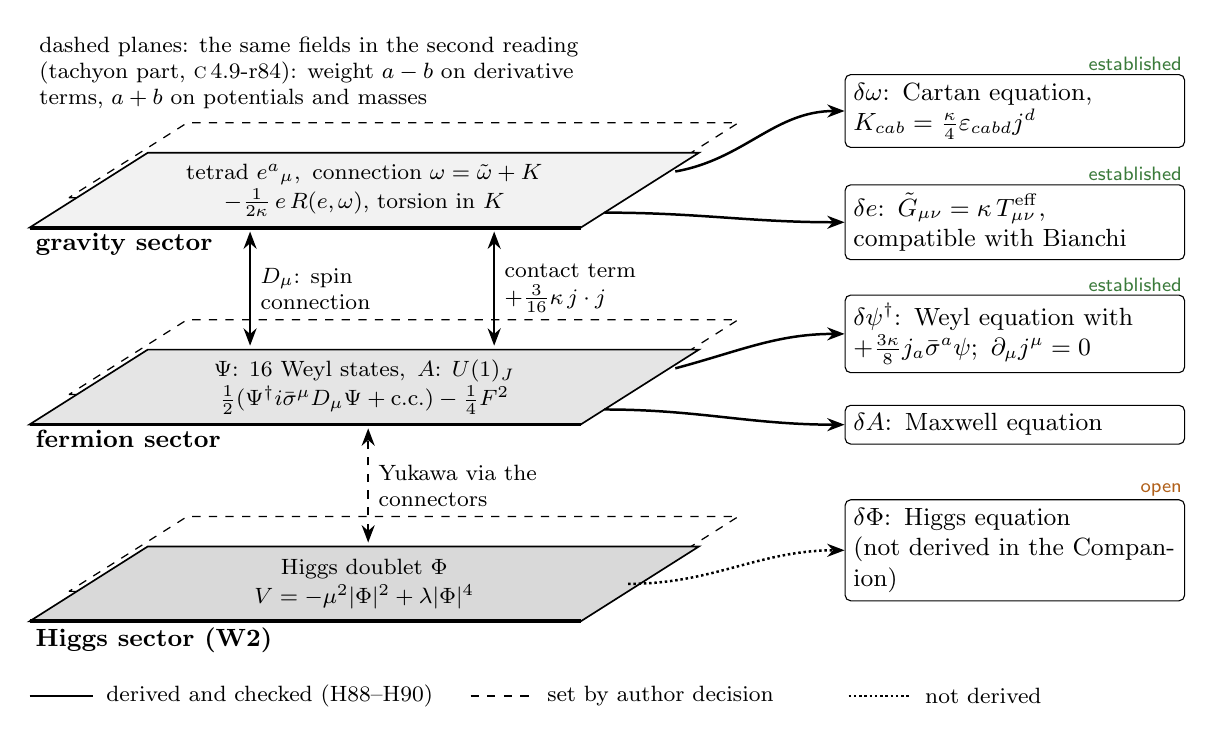
\begin{tikzpicture}[font=\small,>={Stealth[length=2.2mm]},
  plane/.style={draw=black,line width=0.6pt},
  fld/.style={align=center,inner sep=1.5pt,font=\footnotesize},
  eqbox/.style={draw,rounded corners=2pt,align=left,inner sep=3pt,text width=4.1cm,fill=white},
  tag/.style={anchor=south east,font=\scriptsize\sffamily,inner sep=1pt},
  chk/.style={line width=0.9pt},                % derived and checked
  set/.style={line width=0.9pt,dashed},         % set by author decision
  unc/.style={line width=0.9pt,densely dotted}  % not derived in the Companion
]
% geometry of a sector plane: width W, depth offset (dx,dy); shadow offset (sx,sy) for the second reading
\def\W{7.0}\def\dx{1.5}\def\dy{0.95}\def\sx{0.5}\def\sy{0.38}
\newcommand{\actsectorplane}[3]{% #1 = y offset, #2 = fill gray level, #3 = name
  \draw[dashed,line width=0.45pt,fill=white] (\sx,#1+\sy) -- (\W+\sx,#1+\sy) -- (\W+\dx+\sx,#1+\dy+\sy) -- (\dx+\sx,#1+\dy+\sy) -- cycle;
  \fill[black!#2] (0,#1) -- (\W,#1) -- (\W+\dx,#1+\dy) -- (\dx,#1+\dy) -- cycle;
  \draw[plane] (0,#1) -- (\W,#1) -- (\W+\dx,#1+\dy) -- (\dx,#1+\dy) -- cycle;
  \draw[line width=1.4pt] (0,#1) -- (\W,#1);   % heavier front edge: depth cue
  \node[anchor=north west,font=\small\bfseries,inner sep=2pt] at (0,#1) {#3};}
% the three sectors, back planes lighter
\actsectorplane{0}{15}{Higgs sector (W2)}
\actsectorplane{2.5}{10}{fermion sector}
\actsectorplane{5.0}{5}{gravity sector}
\node[anchor=south west,align=left,font=\footnotesize] at (0,5.0+\dy+\sy+0.05)
  {dashed planes: the same fields in the second reading\\
   (tachyon part, \textsc{c}\,4.9-r84): weight $a-b$ on derivative\\
   terms, $a+b$ on potentials and masses};
% field contents at the plane centres
\node[fld] (G) at (0.5*\W+0.5*\dx,5.0+0.5*\dy) {tetrad $e^a{}_\mu$,\enspace connection $\omega=\tilde\omega+K$\\[1pt] $-\tfrac1{2\kappa}\,e\,R(e,\omega)$, torsion in $K$};
\node[fld] (F) at (0.5*\W+0.5*\dx,2.5+0.5*\dy) {$\Psi$: 16 Weyl states,\enspace $A$: $U(1)_J$\\[1pt] $\tfrac12(\Psi^\dagger i\bar\sigma^\mu D_\mu\Psi+\mathrm{c.c.})-\tfrac14F^2$};
\node[fld] (H) at (0.5*\W+0.5*\dx,0.5*\dy) {Higgs doublet $\Phi$\\[1pt] $V=-\mu^2|\Phi|^2+\lambda|\Phi|^4$};
% couplings between the planes
\draw[chk,<->] (2.8,2.5+\dy+0.05) -- node[right,align=left,font=\footnotesize]{$D_\mu$: spin\\connection} (2.8,4.95);
\draw[chk,<->] (5.9,2.5+\dy+0.05) -- node[right,align=left,font=\footnotesize]{contact term\\$+\tfrac{3}{16}\kappa\,j\cdot j$} (5.9,4.95);
\draw[set,<->] (4.3,\dy+0.05) -- node[right,align=left,font=\footnotesize]{Yukawa via the\\connectors} (4.3,2.45);
% variations and field equations (right column)
\begin{scope}[xshift=10.35cm]
\node[eqbox,anchor=north west] (E1) at (0,6.95) {$\delta\omega$:\enspace Cartan equation,\\ $K_{cab}=\tfrac\kappa4\varepsilon_{cabd}j^d$};
\node[eqbox,anchor=north west] (E2) at (0,5.55) {$\delta e$:\enspace $\tilde G_{\mu\nu}=\kappa\,T^{\rm eff}_{\mu\nu}$,\\ compatible with Bianchi};
\node[eqbox,anchor=north west] (E3) at (0,4.15) {$\delta\psi^\dagger$:\enspace Weyl equation with\\ $+\tfrac{3\kappa}{8}j_a\bar\sigma^a\psi$;\enspace $\partial_\mu j^\mu=0$};
\node[eqbox,anchor=north west] (E4) at (0,2.75) {$\delta A$:\enspace Maxwell equation};
\node[eqbox,anchor=north west] (E5) at (0,1.55) {$\delta\Phi$:\enspace Higgs equation\\ (not derived in the Companion)};
\end{scope}
\draw[chk,->] (\W+\dx-0.3,5.0+0.75*\dy) to[out=10,in=180] (E1.west);
\draw[chk,->] (\W+0.3,5.0+0.2*\dy) to[out=0,in=180] (E2.west);
\draw[chk,->] (\W+\dx-0.3,2.5+0.75*\dy) to[out=15,in=180] (E3.west);
\draw[chk,->] (\W+0.3,2.5+0.2*\dy) to[out=0,in=180] (E4.west);
\draw[unc,->] (\W+0.6,0.5*\dy) to[out=0,in=180] (E5.west);
% status tags above the boxes
\node[tag,text=st-est] at (E1.north east) {established};
\node[tag,text=st-est] at (E2.north east) {established};
\node[tag,text=st-est] at (E3.north east) {established};
\node[tag,text=st-open] at (E5.north east) {open};
% legend
\begin{scope}[yshift=-0.95cm]
\draw[chk] (0,0) -- (0.8,0); \node[anchor=west,font=\footnotesize] at (0.85,0) {derived and checked (H88--H90)};
\draw[set] (5.6,0) -- (6.4,0); \node[anchor=west,font=\footnotesize] at (6.45,0) {set by author decision};
\draw[unc] (10.4,0) -- (11.2,0); \node[anchor=west,font=\footnotesize] at (11.25,0) {not derived};
\end{scope}
\end{tikzpicture}
\caption{The action W1/W2 as three sector planes \Conditional. Gravity (tetrad and independent connection with torsion,
corrected sign of $R$), the fermions stored in the Dixon carrier with the gauge field of $U(1)_J$, and the Higgs doublet of
W2. Vertical arrows are couplings: the spin connection in $D_\mu$, the contact term left by eliminating torsion, and the
Yukawa couplings through the connectors, whose form and the sign of $-\mu^2$ are set, not derived. The right column shows
which field equation follows from which variation; the first three were derived independently in Wolfram Language and
in a jet computation (\rndold{r86}, \rnd{r01}); the Maxwell equation was imposed there, not tested separately. The dashed planes behind are the tachyon part as a second reading of the
same fields (\rndold{r84}). Line styles carry the status in black and white.}
\label{fig:act-scheme}
\end{figure}


\subsection{Field equations, derived independently}
\label{sec:act-equations}

The first derivations (\rndold{r81}) were Python and sympy scripts written in the same sessions. In \rndold{r86} a second
system, Wolfram Language, derived the field equations from their definitions (pre-registered tests H88, H89, not blind,
since the expected forms were known), and \rnd{r01} closed the last gap with the fully non-linear Einstein--Cartan
equation (H90, not blind). We state the results for the corrected action~\eqref{eq:act-W1}; Section~\ref{sec:act-sign}
lists the sign changes relative to the action as first written.

\begin{proposition}[Field equations of W1; \rndold{r86}, \rnd{r01}]
\label{prop:act-fieldeq}
For the action \eqref{eq:act-W1}, with $j^a=\sum\Psi^\dagger\bar\sigma^a\Psi$ the total current of all sixteen states:
\begin{enumerate}
\item[(a)] \emph{Generator.} $\Sigma^{ab\dagger}\bar\sigma^c+\bar\sigma^c\Sigma^{ab}=-(\eta^{bc}\bar\sigma^a-\eta^{ac}\bar\sigma^b)$, hence
  $D_\mu j^c=\partial_\mu j^c+\omega_\mu{}^c{}_b\,j^b$; the ordering $\tfrac14(\bar\sigma^a\sigma^b-\bar\sigma^b\sigma^a)$ is not covariant.
\item[(b)] \emph{Cartan equation.} The $\omega$-equation is solved by $\omega=\tilde\omega+K$, with $\tilde\omega$ the torsion-free
  connection of the tetrad and the totally antisymmetric contorsion
  \begin{equation}
  K_{cab}=\frac{\kappa}{4}\,\varepsilon_{cabd}\,j^d .
  \label{eq:act-contorsion}
  \end{equation}
\item[(c)] \emph{Elimination of torsion.} Inserting (b) gives the four-fermion contact term
  \begin{equation}
  \mathcal L_{4f}=+\frac{3}{16}\,\kappa\,j\cdot j ,
  \label{eq:act-4f}
  \end{equation}
  with the total current; the torsion is blind to the $U(1)$ charge. For a single Weyl spinor the term vanishes, since its
  current is null.
\item[(d)] \emph{Weyl equation.} Varying with respect to $\psi^\dagger$ gives
  $i\bar\sigma^\mu\partial_\mu\psi-qJA_\mu\bar\sigma^\mu\psi+\tfrac{3\kappa}{8}\,j_a\bar\sigma^a\psi=0$ (written in the local
  form of the check).
\item[(e)] \emph{Current conservation.} The operator $M=qJA_\mu\bar\sigma^\mu-\tfrac{3\kappa}{8}j_a\bar\sigma^a$ is hermitian,
  hence $\partial_\mu j^\mu=0$ on solutions (Ward identity).
\item[(f)] \emph{Einstein--Cartan equation.} The tetrad variation at $\omega=\tilde\omega+K$ is symmetric on the field
  equations and gives, fully non-linearly,
  \begin{equation}
  \tilde G_{\mu\nu}=\kappa\,T^{\mathrm{eff}}_{\mu\nu},\qquad
  T^{\mathrm{eff}}_{\mu\nu}=T^{\mathrm{Bel}}_{\mu\nu}-g_{\mu\nu}\mathcal L_W+T^{\mathrm{Maxwell}}_{\mu\nu}
    -\frac{3\kappa}{16}\,g_{\mu\nu}\,j\cdot j ,
  \label{eq:act-einstein}
  \end{equation}
  where $\tilde G$ is the Einstein tensor of the Levi-Civita connection, $T^{\mathrm{Bel}}$ the Belinfante tensor and
  $\mathcal L_W$ the Weyl Lagrangian.
\item[(g)] \emph{Compatibility.} $\tilde\nabla^\mu T^{\mathrm{eff}}_{\mu\nu}=0$ on the field equations, consistent with the Bianchi
  identity $\tilde\nabla^\mu\tilde G_{\mu\nu}=0$.
\end{enumerate}
\end{proposition}

\begin{proof}[How it was checked]
(a), (c)--(e) were derived symbolically in Wolfram Language from the definitions: all $64$ components of the generator
identity, all $24$ contorsion components for two Weyl spinors (\rndold{r86}, r86.2). (b), (f), (g) were computed in
\rnd{r01} at a generic point of three random curved backgrounds (tetrad a random non-diagonal polynomial of degree three),
with all fields carried as jets to third order: three Weyl fields with charges $J=(+1,-1,+1)$, a real potential $A$ and
the tetrad, the spinor jets solving the Weyl equation with gauge and four-fermion terms at the point and to first
derivative. The residuals are $\le2\times10^{-14}$ for the Cartan equation, $10^{-15}$ for the Einstein equation and
$4\times10^{-15}$ (relative) for the divergence. Negative controls fail as they should: without the four-fermion term the
residuals rise to $0.12$--$0.19$ (Einstein) and $0.25$--$0.81$ (divergence); with spinors off the field equations to
$0.16$--$0.19$ and $0.92$--$1.05$. In addition, the first-order tetrad variation around flat space, with the spin
connection solved from $de+\omega\wedge e=0$ rather than inserted, equals minus the Belinfante tensor on a solution of
two plane waves, exactly symmetric, to $7\times10^{-15}$ (\rndold{r86}, r86.3(c)).
\end{proof}

These are numerical-exact checks at generic points, not a general symbolic proof of~(f); the round records them as such,
together with two errors found in the checking code (a conjugate transpose that also conjugated real symbols, and extra
$\eta$ factors in $\omega_{\mu ab}\Sigma^{ab}$). After their correction everything agreed; the disagreement lay in the
checking code, not in W1 (\rndold{r86}, disclosure to r86.3). The modulus $3/16$ of~\eqref{eq:act-4f} is the
Hehl--Datta value \cite{D:HehlDatta}, which the control of \rndold{r81} reproduced for a Dirac field.

\subsection{The sign of the gravitational action}
\label{sec:act-sign}

The non-linear computation of \rnd{r01} carried the sign of the gravitational term as a parameter,
$S_{\mathrm{grav}}=\frac{\sigma_g}{2\kappa}\int e\,R$, and found $\tilde G=-\sigma_g\kappa T^{\mathrm{eff}}$. For W1 as written
in \rndold{r81} ($\sigma_g=+1$) the factor is $-1$ to $4\times10^{-15}$. A weak-field computation in Wolfram fixes which
sign attracts: for $g=\mathrm{diag}\bigl(1+2\Phi,-(1-2\Phi)\mathbf 1\bigr)$ in the same curvature convention one finds
$G_{00}=2\nabla^2\Phi$. With $T_{00}=\rho>0$, $\tilde G=+\kappa T$ gives $\nabla^2\Phi=\kappa\rho/2=4\pi G\rho$ for
$\kappa=8\pi G$, which is Newtonian attraction, while $\tilde G=-\kappa T$ is repulsion. \Refuted\ W1 as first written
repels positive energy. The earlier Hehl--Datta control had compared only the modulus $3/16$, not the sign.

On 6~November 2026 the author corrected the action to~\eqref{eq:act-W1} (\rnd{r01}, decision r01.2). Moduli and forms of
all derived terms stay; the signs that change are (r01.3):
\begin{itemize}
\item the contact term becomes $\mathcal L_{4f}=+\tfrac3{16}\kappa\,j\cdot j$ and the Weyl-equation term
  $+\tfrac{3\kappa}{8}j_a\bar\sigma^a\psi$ (both were negative), the contorsion $K_{cab}=+\tfrac\kappa4\varepsilon_{cabd}j^d$;
\item the four-fermion stress becomes $T^{(4f)}_{\mu\nu}=-\tfrac{3\kappa}{16}\,j^2g_{\mu\nu}$ (Section~\ref{sec:act-stiff});
\item \emph{the torsion pairing channel becomes repulsive.} By the Fierz identity
  $\bar\sigma^\mu_{ab}\bar\sigma_{\mu\,cd}=2\varepsilon_{ac}\varepsilon_{bd}$ one has $j_1\cdot j_2=2|\Phi|^2$ for the Lorentz-scalar pair
  $\Phi=\psi_2^{\mathsf T}\varepsilon\psi_1$ (\rndold{r82}, r82.4). With the physical sign the interaction contains
  $H_{\mathrm{int}}\supset+\tfrac34\kappa\,\Phi^\dagger\Phi$; no condensate forms through it. The Planck-scale $\nu^c$
  Majorana condensate and the seesaw estimate that \rndold{r82} had drawn from the attractive sign are withdrawn.
\end{itemize}
Tests that do not involve the sign of the gravitational coupling are unaffected; \rnd{r01} lists them (r01.3(e)).

\subsection{A homogeneous fermion state is stiff matter, not a vacuum term}
\label{sec:act-stiff}

Since $T^{(4f)}_{\mu\nu}=-g_{\mu\nu}\mathcal L_{4f}$, the contact term taken \emph{on its own} has the algebraic form of a
cosmological term. In signature $(+,-,-,-)$ and a local rest frame,
\begin{equation}
\rho_{4f}=T^{(4f)}_{00}=-\mathcal L_{4f}=-\frac{3\kappa}{16}\,j^2,\qquad
p_{4f}=T^{(4f)}_{ii}=+\mathcal L_{4f}=-\rho_{4f},
\label{eq:act-4f-stress}
\end{equation}
a negative vacuum-like term, but with a height $\propto j^2$ that is not constant (\rndold{r86}, r86.3(a); sign after
\rnd{r01}). It cannot be separated physically from the kinetic part. For the whole tensor the answer is different:
two Weyl fields of opposite spin with a homogeneous phase solve the Weyl equation of
Proposition~\ref{prop:act-fieldeq}(d) exactly, with total current $(n,0,0,0)$, and on this solution the whole tensor
$T_{\mu\nu}=T^{\mathrm{Bel}}_{\mu\nu}-g_{\mu\nu}\mathcal L$ has
\begin{equation}
\rho=p=-\frac{3\kappa}{16}\,n^2 ,
\label{eq:act-stiff}
\end{equation}
that is, stiff matter ($w=1$) with the negative spin energy density known from Einstein--Cartan theory (\rndold{r86},
r86.3(b); \rnd{r01}, r01.3(b)). \Established\ (for W1 as stated) The homogeneous fermion state is stiff matter, not
$\Lambda$; W1 still produces no vacuum term.

\subsection{The tachyon image of an action}
\label{sec:act-image}

The Companion's frames M and T are related by the tachyon map, which on rapidities is the continuation
$\eta\mapsto\eta+i\pi/2$ (Convention F; it is not time reversal, and on the field doublet it is the electromagnetic
duality, not a Wick rotation). For a single momentum this is clear; for an \emph{action} it had not been fixed. Round
\rndold{r83} compared three readings for a scalar with $L_M=\tfrac12(\chi_t^2-\chi_x^2)-\tfrac12m^2\chi^2$ against three
criteria fixed in advance (pre-registered test H77, not blind): K1 tachyonic dispersion, as the frame map requires;
K2 $L_T=-L_M$ for massless fields, as in \rndold{r81}; K3 a running mode of the image carries energy of the opposite sign.

\begin{center}
\small
\begin{tabular}{@{}l>{\raggedright\arraybackslash}p{0.36\textwidth}lccc@{}}
\toprule
reading & rule & dispersion & K1 & K2 & K3\\
\midrule
A & $L_T=-L_M$ (energy parity) & $\omega^2=k^2+m^2$ & no & yes & yes\\
B & kinematics continued, $X\mapsto-X$, constants and potentials kept & $\omega^2=k^2-m^2$ & yes & yes & yes\\
B$'$ & $m^2\mapsto-m^2$ with real kinematics & $\omega^2=k^2-m^2$ & yes & no & no\\
\bottomrule
\end{tabular}
\end{center}

\noindent Only reading B is compatible; reading A is a ghost copy with normal dispersion. In reading B a potential without
derivatives keeps its sign, so the tachyonic Higgs mass of M is a normal mass in the image and the image does not
condense. The cancellation of the Higgs vacuum energy at photon weights that \rndold{r82} had found in reading A
therefore does not hold and was withdrawn; the vacuum energy is $a\,V_{\min}$ (\rndold{r83}, correction to r82.1).

\paragraph{Second reading of the same field.} If the tachyon part were an independent field, the vacuum of matter plus
image would decay through graviton exchange, $0\to\varphi\varphi\chi\chi$, at a rate that is unbounded without a preferred
frame; with a frame cutoff the gamma-ray background bounds the cutoff to about $14\,\mathrm{MeV}$ (\rndold{r83}, H76, not
blind; the scaling is that of \cite{D:Cline}). On 5~November 2026 the author decided instead that the tachyon part is
\emph{the same field in a second reading} (\rndold{r84}). The map is the complete complex boost with rapidity $i\pi$:
\begin{equation}
S(\theta)=e^{-\theta\sigma_z/2},\quad S\bar\sigma^\mu S=\Lambda(\theta)^\mu{}_\nu\bar\sigma^\nu,\qquad
S(i\pi)=-i\sigma_z,\quad \Lambda(i\pi)=\mathrm{diag}(-1,1,1,-1),
\label{eq:act-boost}
\end{equation}
acting on the spinor index \emph{and} on the argument, $\psi_T(x)=S\,\psi(\Lambda x+\delta)$. With the adjoint mapped
holomorphically, $\psi^\dagger\mapsto\psi^\dagger S$, the image term is $-L_M$ in all four directions, and the weighted action
is $(a-b)S_M$: isotropic, stable for $a>b$, with opposite energy in the image (criterion K3). The hermitian alternative
$\psi^\dagger\mapsto\psi^\dagger S^\dagger$ gives $(a+b)S_M$ and violates K3 (H79, not blind). The author fixed the holomorphic
form; in the matter reading the Dirac adjoint stays. A first form that rotated only the spinor index gave an anisotropic
Weyl operator with factor $(a+b)/(a-b)=\gamma_L=1.8645$ at matter weights, a Lorentz violation of order one for fermions
that laboratory bounds exclude (H78; \cite{Altschul2010}).

For a scalar the weighted Lagrangian is
\begin{equation}
a\,L_M+b\,L_T=(a-b)\,\tfrac12X-(a+b)\,V ,
\label{eq:act-weights}
\end{equation}
independent of the offset $\delta$ in flat space. Terms with derivatives enter with $a-b$, mass terms (Dirac and
Majorana masses are invariant under the complete boost) with $a+b$ (\rndold{r85}, H82). Photon weights are $a=b$; matter
weights have $b/a=\bsym^2$, so that $(a-b)/(a+b)=1/\gamma_L$. Since there are no independent T quanta, the decay channel
of H76 does not exist. \Conditional\ As a second reading of the same field, formed by the complete complex boost with
holomorphic adjoint, the tachyon part is isotropic, stable for $a>b$ and free of vacuum decay. This supports the
construction, not the physical identity of matter and tachyon sector (thesis T1 stays a conjecture). In flat space the
second reading only renormalises the kinetic term against the potential; the vacuum energy is cancelled in no variant.

\subsection{What the action does not supply}
\label{sec:act-noscale}

\Open\ The only scale W1 and W2 bring with them is the Planck scale; $\mu$ and $\lambda$ of W2 are inputs
(\rndold{r82}, consequence). A $\Lambda$-like term can arise from tachyonic modes of both norm signs, but its height and
sign are set by a free weight ratio (\rndold{r81}, H72); with the second reading no tachyonic branch remains, and every
route examined in \rnd{r03} and \rnd{r04} ends with a vacuum term that is a free multiple of $V_{\min}$. The aim of the
programme, a vacuum term that is not free, is not met (\rnd{r05}, r05.2(c)); Section~\ref{sec:lop5} states the corresponding negative
result for $\Lambda$ in the full class of constructions of the Companion. Table~\ref{tab:act-status} collects the status.

\begin{table}[ht]
\centering
\small
\begin{tabularx}{\textwidth}{@{}>{\raggedright\arraybackslash}X>{\raggedright\arraybackslash}p{0.43\textwidth}l@{}}
\toprule
statement & status & source\\
\midrule
action W1, $U(1)_J$ anomaly-free on the full carrier & \Conditional\ set up under author decisions & \rndold{r81}\\
field equations (generator, torsion, Weyl, Ward) & \Established\ for W1, derived in Wolfram (H88) & \rndold{r86}\\
non-linear Einstein--Cartan equation, Bianchi & \Established\ for W1, derived and compatible (H90) & \rnd{r01}\\
sign of the gravitational action & \Refuted\ as first written (repulsion); corrected by author decision & \rnd{r01}\\
torsion pairing channel & repulsive after the correction; Planck-scale condensate withdrawn & \rnd{r01}\\
homogeneous fermion state & stiff matter, $\rho=p<0$; not a vacuum term & \rndold{r86}, \rnd{r01}\\
tachyon image of an action & reading B (kinematics continued); A excluded (H77) & \rndold{r83}\\
tachyon part as second reading & \Conditional\ isotropic, stable, no vacuum decay (H79) & \rndold{r84}\\
Higgs vacuum energy with image & no cancellation, $a\,V_{\min}$ & \rndold{r83}\\
own scale, value of $\Lambda$ & \Open\ none supplied; programme frozen & \rnd{r05}\\
\bottomrule
\end{tabularx}
\caption{Status of the action programme W1/W2. ``Established'' refers to the derivation for the stated action, not to
the action as physics.}
\label{tab:act-status}
\end{table}

\subsection{The Big Bang: an exploration}
\label{sec:act-bang}

\Exploration\ The second reading suggests a picture of the Big Bang, which the Companion has explored; most tests on it
were pre-registered but not blind. By a further author decision, the domain choice G2 of \rndold{r85}, the matter reading
lives after the Big Bang and the tachyon reading on its image before it, joined only at $\tau=0$. Structurally this is the
two-sheet picture of the CPT-symmetric universe of Boyle, Finn and Turok \cite{D:BFT}; the resemblance was noticed
afterwards.

\paragraph{What is shown.}
\begin{itemize}
\item \emph{A CPT-like transition with an admixture fixed by $\bsym$} (\rndold{r85}). For conformal fields the weight jumps
  from $-b$ to $a$. In the sharp limit a positive-norm mode before the bang becomes
  $C\,e^{-i\omega\tau}+D\,e^{+i\omega\tau}$ with $C=(a+b)/(2a)$, $D=(a-b)/(2a)$; normalised, the Bogoliubov ratio is
  $|\beta/\alpha|=1/\gamma_L=0.536$ and the occupation $n=(1-\bsym^2)^2/(4\bsym^2)=0.404$ per mode, for every $k$; at photon
  weights $n=0$. With a smooth transition of duration $\Delta$, taken around zero in the complex plane, every mode of the
  tachyon reading is mapped to a mode of negative frequency after the bang (a CPT assignment), and the admixture is cut
  off exponentially for $k\Delta\gg1$ (H86; checked by a second system in \rndold{r86}). $\Delta$ is a free scale.
\item \emph{Fermions pass without admixture} (\rnd{r03}). The weighted Dirac or Weyl equation is solved exactly by
  $\psi=c^{-1/2}\chi$ with $\chi$ free, for every profile $c(\tau)$; positive and negative frequencies do not mix, and the
  transfer factor is $\pm i\bsym$, unitary in the weighted norm. A first-order equation lets the weight be scaled away; the
  second-order equations of bosons do not. On an expanding background this holds for $k\gg m\,a(\tau)$ at the transition.
\item \emph{Bosons are norm-preserving only far from $1/\Delta$} (\rnd{r03}, H94). For $k\Delta\ll1$ they pass as a
  Bogoliubov transformation, for $k\Delta\gg1$ they are CPT-mirrored; in between the transition is not norm-preserving.
  The author set $\Delta\lesssim\ell_P$, which moves that range to the Planck scale.
\item \emph{No $\Lambda$ from the tachyon sector after the bang} (\rnd{r03}, \rnd{r04}). Under G2 only the matter reading
  exists after the bang, so neither the tension of a matter--tachyon mixture nor a tachyonic or ghost condensate survives
  it. A vacuum term after the bang can only be $a\,V_{\min}$ of the matter reading, with a free value. Admitting the
  tachyonic branch as degrees of freedom of its own did not help either (H95 refuted), and that admission was withdrawn.
  $\Lambda$ stays an input.
\end{itemize}

\paragraph{What could still be.} \Open\ Whether the transition has a physical duration $\Delta$ and what fixes it; what
the two senses of the complex rotation mean (they are exactly conjugate and give an asymmetry with fixed product); how
tensor modes see the transition, which an observable trace such as a gravitational-wave background would need; and the
energy in bosons created near $k\sim1/\Delta$, which sets a Planck-hot, non-thermal start without fermions and an open
problem for $\Delta N_{\mathrm{eff}}$ (\rnd{r04}, \rnd{r05}). None of this is derived. The picture is a consistent reading
of the second reading under G2, not a result about the early universe.

% Section 8 (group C): Lambda and OP5, negative results
\section{\texorpdfstring{$\Lambda$}{Lambda} and OP5: negative results}
\label{sec:lop5}

This section reports what the construction does \emph{not} deliver for the cosmological constant.  The results are mostly negative: no
equation in the constructions of the Companion selects a value of $\Lambda$, the one dynamics that would produce the ratio $\Omega_M=\bsym^2$
either fails the data (H97) or puts that ratio in the future (H124), and the mediator that the local OP5 comparison model needs is causally
incompatible with the Higgs sector of the action W2.  The readout prediction H96 is open and will be decided by data.

\subsection{Two questions under one name}
\label{sec:lop5-split}

OP5 had two meanings in the Companion (\rnd{r05}, Decision~5.3).  In the architecture of the core it is the reversal-stable return readout of a
route whose source readout is OP1.  In physics it is the question of $\Lambda$, read in the core as a branching of a cascade,
$\Omega_\Lambda:\Omega_M=(1-\bsym^2):\bsym^2$, not as a dynamical vacuum energy (\cite{QSC}, \texttt{thm:dark-energy}).  On 6 November 2026 the
author separated three parts:
\begin{enumerate}
\item \emph{OP5 (core):} the reversal closure of the source--return pair.  It holds as a conditional schema under the assumptions of
\texttt{thm:op15-closure}; no native instance of the route with evaluable transports, class test and readout exists (\rnd{r11}, Theoremlet~11.2(a)).
\item \emph{$\Lambda$ readout:} whether $\Omega_\Lambda:\Omega_M=(1-\beta^2):\beta^2$ is the cascade branching, and at which epoch.  The epoch was fixed as
the present.
\item \emph{Action programme W1/W2:} a separate branch, frozen (Section~\ref{sec:act}).
\end{enumerate}
The historical chain that led from a spectral carrier through a trace formula to a bare $\Lambda$ term and a cancellation task lacks the step to a
well-defined metric action, and the size of the bare term does not follow.  The author suspended it as a foundation (\rnd{r11}, Decision~11.1).  The
working question since then is which independently defined quantity can be obtained by an explicit readout of the core, and which checkable
constraint follows.

Even the cascade only stabilises the ratio.  In the Markov cascade of the Companion the outflow fraction returns its input
$q=\lambda_-/\lambda_+=\tanh^2\eta$ for every rate; it does not derive it.  The register algebra admits a family of fields with any $0<q<1$ in the same
sector, so it does not select $q$ either (\rnd{r11}, Theoremlet~11.2(b),(c)).  The identification $q=\Omega_M(\text{today})$ is an additional assumption.

\subsection{H96 and H97}
\label{sec:lop5-h96}

Once the pair of counting rules is chosen, the $\Lambda$ readout gives a prediction without a free parameter (pre-registered; \rnd{r05}, Theoremlet~5.4):
\begin{equation}
 \Omega_M=\bsym^2=\frac{\gamma_L-1}{\gamma_L+1}=0.30185 .
 \label{eq:lop5-h96}
\end{equation}
It is decided by the first flat-$\Lambda$CDM value of $\Omega_m$ published after 6 November 2026 from DESI DR3 (BAO alone) or from Euclid,
confirmed within $2\sigma$.  The known values, DESI DR2 $0.2975\pm0.0086$ \cite{DESIDR2} ($0.5\sigma$) and Planck $0.3153\pm0.0073$
\cite{Planck2018}, are disclosed and do not count.  H96 rests on the U(1) counting per frame of Section~\ref{sec:beta} and on reading $\gamma_L$ as a
Lorentz factor.  Status \Open; no decisive data existed on 22 November 2026 (\rnd{r31}, Remark~31.6).

The only dynamics for the ratio in the Companion is the cascade with a return path.  A proposed bridge to cosmic time lets vacuum energy decay
into matter at the rate $\beta^2\Gamma$ with $\Gamma=\varepsilon H$.  With $\varepsilon=1$ it has no free parameter.  Test H97 (pre-registered,
not blind) compared it with the 13 DESI DR2 BAO values: $\chi^2_{\min}=105.0$ for 12 degrees of freedom, $p=6\times10^{-17}$.  H97 is
\Refuted.  The control, flat $\Lambda$CDM with free $\Omega_m$, reproduces DESI ($\Omega_m=0.2970$), and flat $\Lambda$CDM at $\Omega_M=\beta^2$ has
$\chi^2=10.9$, $p=0.54$ (\rnd{r05}, Theoremlet~5.5).

\subsection{The OP5 comparison model: a worked case}
\label{sec:lop5-worked}

The OP5 comparison model is a local auxiliary construction: a reduced field theory in which a matter modulation drives a comparison field whose
response can be read along a ray.  The worked case of \rnd{r32} collects its derivations; the algebraic steps (Theoremlets~32.2 and 32.4--32.6) were checked exactly in Wolfram Language.

\paragraph{What is chosen.}
Two inputs are set.  (i) The drive operator
\begin{equation}
 \mathcal P(\omega,\mathbf k)=\frac{\bigl[Z(\Omega_0^2+c_h^2q-x)+\tfrac32g_0^2d\bigr]d_m-g_m^2N_m}{m^2},
 \qquad N_m=\tfrac23\bigl(x^2-a_\perp x+a_\perp^2\bigr),
 \label{eq:lop5-drive}
\end{equation}
with $x=\omega^2$, $q=|\mathbf k|^2$, $a_\perp=|\mathbf k_\perp|^2$, $d=q-x$, $d_m=m^2+r_mq-x$.  It comes from a directed massive mediator of mass
$m$ plus the Einstein channel; the coefficients are chosen (one checked choice: $Z=1$, $r_m=c_h^2=\tfrac12$, $g_0^2=g_m^2=3/100$).
(ii) The identification of the radial Higgs source of matter with the drive of the comparison field, $\delta J_{\mathrm{OP5}}=\delta\mathcal J_h$.  It would
follow from a coupling $\int h\,\mathcal J_h$ in the same action that produces $\mathcal P$; no such action exists.

\paragraph{What follows.}
With the Higgs radius $h_{\mathrm W}=v+\eta_h$ of W2 and masses $m_i=y_ih_{\mathrm W}$, the radial source of non-relativistic matter is
$\mathcal J_h=-\sum_iy_in_i$, and a displacement $\mathbf u$ gives $\delta\mathcal J_h=(\sum_iy_in_{i0})\nabla\cdot\mathbf u$.  Two superposed elastic
continua with an internal spring can be prepared so that this source is switched on from rest while the energy--momentum tensor stays conserved
(Theoremlets~32.1, 32.2).

\begin{proposition}[compact ordinary response; \rnd{r32}, Theoremlet~32.3]
\label{prop:lop5-compact}
Let $V$ be smooth, spatially compact and zero before the switching, $D_0=\partial_t^2-\Delta$, and choose the preparation so that
$\delta\mathcal J_h=\mathcal P\,\delta H$ with $\delta H=-D_0\Delta^2V$.  Then $\delta T=-D_0T_*$ for a conserved tensor $T_*$ supported where $V$ is,
and in harmonic gauge with zero initial data and no incoming wave the linearised Einstein equation $D_0\bar\gamma_{\mu\nu}=16\pi G\,\delta T_{\mu\nu}$
has the solution $\bar\gamma_{\mu\nu}=-16\pi G\,T_{*,\mu\nu}$.  The ordinary linear curvature vanishes outside the support of $V$, also during
the switching.
\end{proposition}

\begin{proof}[Sketch]
$\delta T$ is linear in the preparation and the operators have constant coefficients, so $\delta T=-D_0T_*$.  Then $D_0(\bar\gamma+16\pi GT_*)=0$
with vanishing past data, whose retarded solution is zero.  Only linearity, constant coefficients and the initial data enter; the identification
(ii) does not.
\end{proof}

Under the identification (ii), the same source gives a non-zero directed contrast on the same axis: for a suitable compact profile with vanishing
transverse integral in every slice, the tidal readout of a ray along the axis is
$\Delta\mathcal I=16\mathcal AP/(m^2R^4)\neq0$, where $\mathcal A$ is the amplitude, $P$ the integrated longitudinal profile and $R$ the transverse
radius (Theoremlet~32.4).  The ordinary exterior is compact \Established; the contrast is \Conditional\ on (ii) and on the chosen
coefficients.  With a normalisation $\delta J_{\mathrm{OP5}}=c\,\delta\mathcal J_h$ the contrast scales with $c$, and whether $c\neq0$ is decided only
by a common action.  The case appears in shorter form in the v5.5.0 physics edition (development subsection ``A worked case'').

Figure~\ref{fig:lop5-slices} shows an earlier numerical object of the same comparison sector: one saved approximate field evaluated on six
coordinate-plane cuts.  It illustrates what the model provides at sampled points (invertible coframes, a nonzero residual) and what it does not
(an exact regional solution).

\begin{figure}[p]
\centering
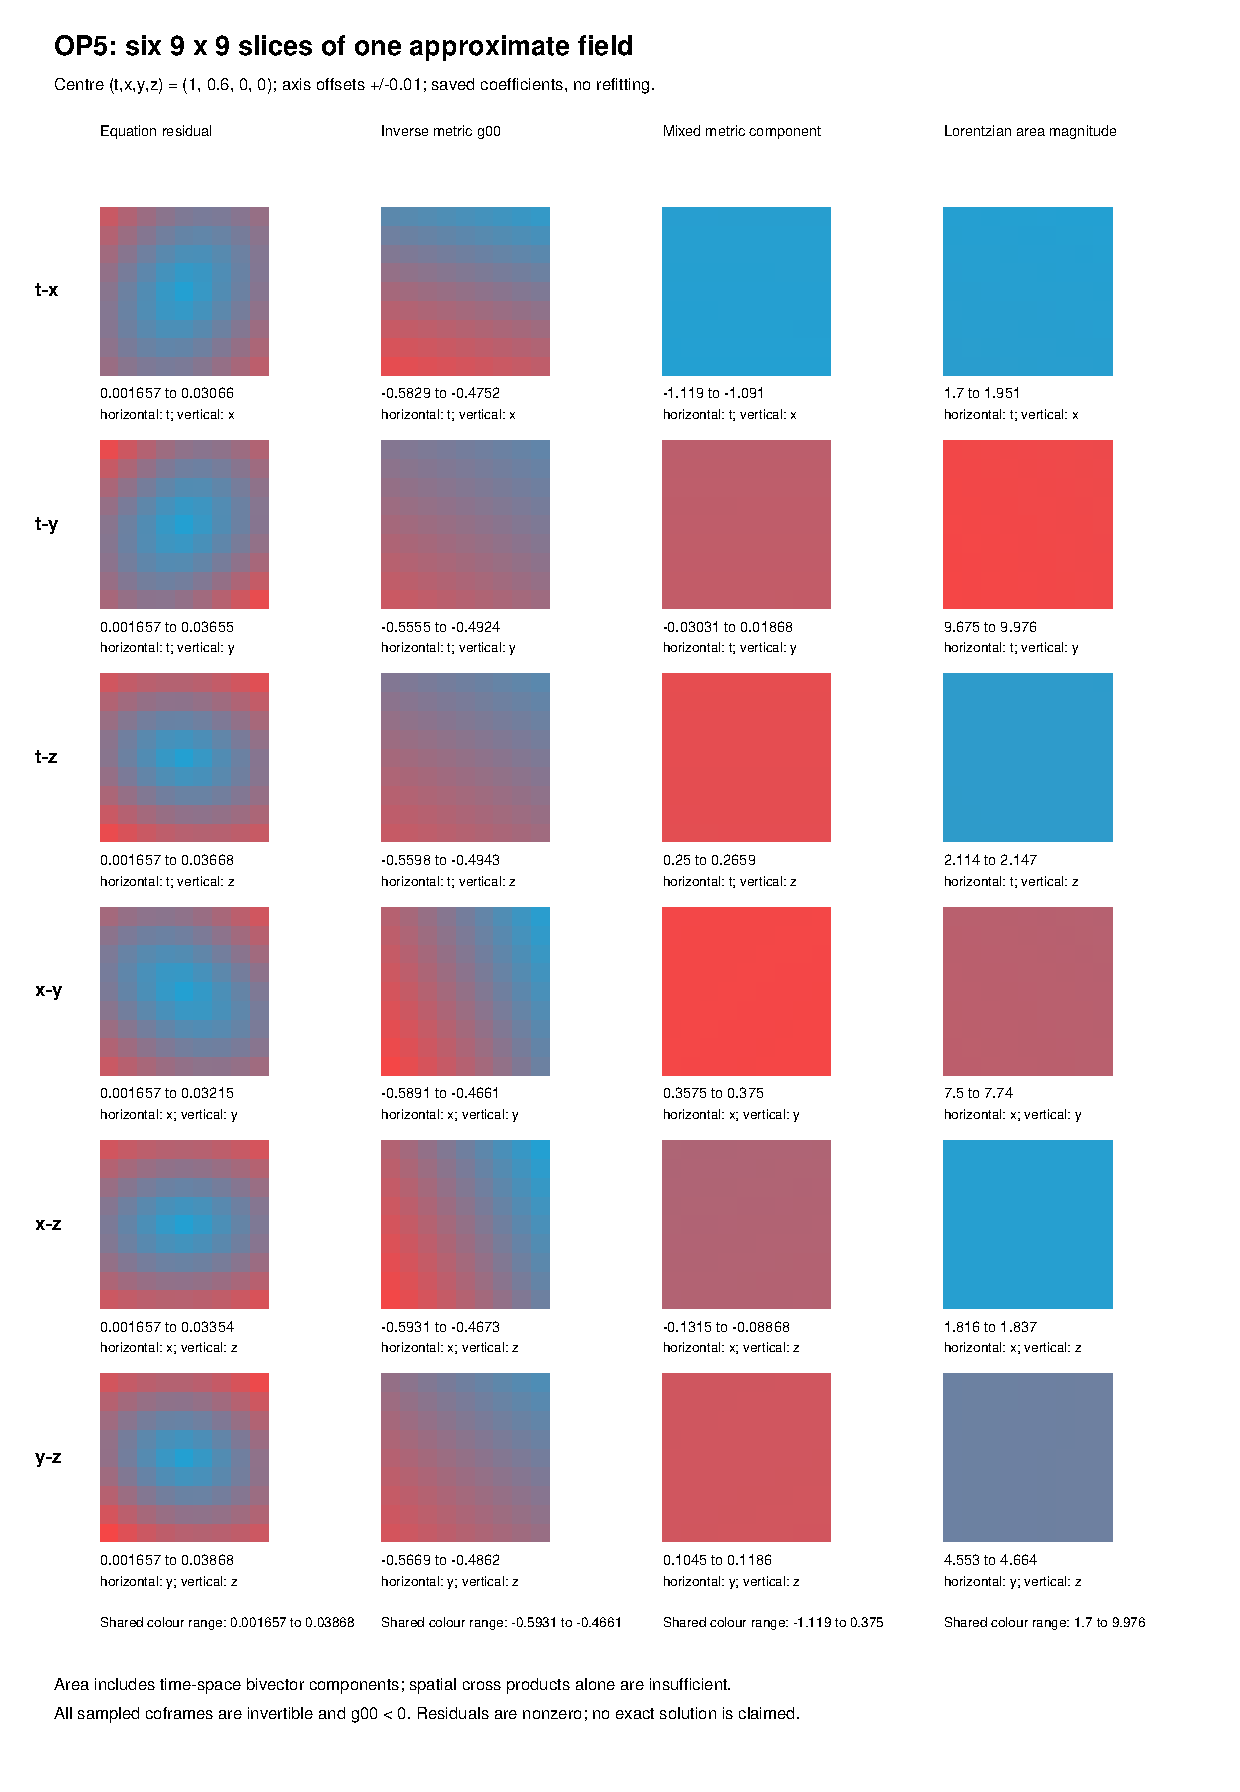
\includegraphics[width=\textwidth,height=0.66\textheight,keepaspectratio]{figures/F9-op5-slices.pdf}
\caption{OP5 comparison field, original affine baseline of 29 October 2026 (\cite{QSC}, subsection on the sampled multimode geometry; it predates
the worked case of \rnd{r32}).  Six overlapping $9\times9$ cuts through $(t,x,y,z)=(1,0.6,0,0)$ with offsets $\pm0.01$ of one saved approximate
field, a sum of two exponential modes, evaluated without refitting.  Columns: full probe-equation residual norm, $g^{00}$, normalised mixed
metric component $g_{ij}/\sqrt{|g_{ii}g_{jj}|}$, Lorentzian area magnitude $\sqrt{|g_{ii}g_{jj}-g_{ij}^2|}$; common colour range per column.
Largest sampled residual $\approx0.0387$, smallest $|\det|$ of the coframe $9.699$, every sampled $g^{00}<0$.  These are finite-sample diagnostics,
not uniform bounds.  Status: the residual is nonzero; no exact regional solution, native action or OP5 closure is claimed.}
\label{fig:lop5-slices}
\end{figure}

\subsection{The mediator line: a no-go}
\label{sec:lop5-mediator}

Rounds \rnd{r33} to \rnd{r52} searched for the mediator behind the directed term of~\eqref{eq:lop5-drive}.  We summarise the outcome.

\paragraph{The directed term needs a distinguished frame.}
W2 itself does not supply the comparison data: for the scalar channel it forces $c_h=1$ and $g_0=g_m=0$, and no subluminal directed massive
mediator exists in W1/W2 (\rnd{r33}, \rnd{r34}).  An audit (\rnd{r45}) traced the directed term to its origin: it is an ordinary Fierz--Pauli
exchange of a set, conserved, directed source $S^{\mu\nu}$, built from a coupling to the curvature component $R_{0i0j}$ transverse to an axis $n$
in a frame $u$.  Indeed $S_{\mu\nu}S^{\mu\nu}-\tfrac13(S^\mu{}_\mu)^2=N_m$, with $S_{\mu\nu}S^{\mu\nu}=a_\perp^2-2a_\perp x+2x^2$ and
$S^\mu{}_\mu=2x-a_\perp$.  Over r33--r44 the number of free choices stayed at one while each round moved it.  What remains set is the directed
coupling with frame $u$ and axis $n$, the slowed propagation $r_m$, and the values: all three are data of a distinguished frame.  This exposes a
fork: these data belong either to a field or medium (field side) or to the readout (observer frame, measuring axis).

\paragraph{The readout side carries the frame but not the slowing.}
Read as a readout, the directed coupling is a transverse tidal readout of a detector moving with $u$, and orientation and slowing drop out of the
leading static contrast (\rnd{r46}).  The branch predicts a dependence on the detector motion of relative size $v^2/c^2$ in the detector velocity $v$, very small at
laboratory velocities.  But the reduced model must also satisfy the metric cone limit, i.e.\ no characteristic propagates faster than the
metric light cone.  In the principal part of the model, $r_0$ and $r_m$ are the squared speeds of the massless and the massive mediator,
$\alpha=a_\perp/q\in[0,1]$, and the mediators couple to the Higgs radius with $j_0^2=\tfrac12g_0^2\alpha^2$ and
$j_m^2=\tfrac23g_m^2(r_m^2-r_m\alpha+\alpha^2)$.  With $Z=1$, $g_0^2=g_m^2=3/100$ the largest squared characteristic speed is $0.675$ for the chosen slow values, but $1.064$
for luminal mediators and $1.199$ with $c_h^2=1$ as W2 forces (\rnd{r47}, Theoremlet~47.1).  A Lorentz-covariant field propagates luminally in
every frame, so the slowing needs a distinguished frame on the field side.  The rest frame R of the field of Convention~F can slow propagation only
across its axis (\rnd{r49}, Theoremlets~49.1, 49.2).

\begin{proposition}[no-go for the luminal Higgs radius; \rnd{r49}, Theoremlet~49.3, found afterwards]
\label{prop:lop5-nogo}
For $c_h^2=1$ the left side of the upper condition of the cone limit of the reduced model, which has to be non-negative, is identically
\[
 -\tfrac23g_m^2(1+r_m-\alpha)-\frac{j_0^2}{1-r_0}-\frac{j_m^2}{1-r_m}<0
\]
for all mediator speeds $r_0,r_m\in(0,1)$, all $\alpha\in[0,1]$ and all $g_m>0$.  With the luminal Higgs radius of W2, the directed coupling
violates the metric cone limit for every choice of mediator.
\end{proposition}

\begin{proof}
All three terms are non-positive for $\alpha\le1<1+r_m$, and the first is strictly negative.  (The Companion checks the substitution with sympy.)
\end{proof}

The identification of the comparison field with the radial mode of W2 and the directed coupling are therefore causally incompatible for every
mediator, on either side of the fork \Refuted.  Three propagations would have to be slowed, and each needs a medium with its own rest vector.

\paragraph{A medium, and a vacuum bound.}
A medium of two light-like counter-streams (an object of the photon frame seen from other frames) can keep the cone limit for observers near the balance of the streams; one stream cannot
(H120, \rnd{r50}).  For any medium with a universal slowing $r=1-\epsilon$ in vacuum the upper cone condition gives (for $Z=1$, $g_0=g_m$) exactly
$\epsilon^2\ge g_m^2\bigl(\tfrac23-\tfrac23\alpha+\tfrac76\alpha^2\bigr)$, sharpest at $\alpha=1$, hence $\epsilon\ge\sqrt{7g_m^2/6}$.  Adopting the
laboratory bound $\epsilon\le10^{-13}$ on Lorentz violation (a bound for electrons \cite{Altschul2010}, used here for the Higgs sector without separate evidence) gives
\begin{equation}
 g_m^2\le\tfrac67\times10^{-26}\approx8.6\times10^{-27},
 \label{eq:lop5-bound}
\end{equation}
so the comparison model with $g_m^2=3/100$ is excluded in vacuum by about 25 orders of magnitude.  An observable directed contrast needs a
material whose rest frame is the preparation.  Reading the medium through the frame map $J_B$ instead does not carry: a medium that narrows the cone
in M widens it in T (cone value $0.803$ in M, $4.66$ for the $J_B$ image), so no medium keeps the limit in both (\rnd{r51}).

\subsection{\texorpdfstring{$\Lambda$}{Lambda} as an input}
\label{sec:lop5-input}

After this the author chose a negative closure of the OP5 remainder (\rnd{r56}; exploration, not blind).  Let $\mathcal K$ be the list of
constructions of the Companion that bear on a vacuum term: the frame maps as passive invertible maps and their dimensionless readouts; the reduced
actions of W1/W2; the semiclassical route from relative entropy; the OP5 comparison model; and the Markov cascade with its bridges to cosmic time.
$\mathcal K$ is a list of the record, not the class of all extensions.

\begin{proposition}[\rnd{r56}, Theoremlets~56.2--56.4]
\label{prop:lop5-input}
\textup{(a)} No construction in $\mathcal K$ has an equation that selects a value of the constant.  In W1/W2 the shift $V\to V+c$ of the potential
leaves the field equation unchanged and adds a $w=-1$ source.  Where the metric equations hold only in their trace-free part, the Bianchi identity and
$\nabla^aT_{ab}=0$ give $R+\kappa T=4\Lambda$ with $\Lambda$ an integration constant; in flat FLRW, $\dot H=-\tfrac\kappa2(\rho+p)$ and
$\dot\rho=-3H(\rho+p)$ imply $\tfrac{d}{dt}\bigl(H^2-\kappa\rho/3\bigr)=0$.
\textup{(b)} $\mathcal K$ fixes only dimensionless numbers of order one and contains no length of its own, whereas $\Lambda\ell_P^2=2.85\times10^{-122}$
(Planck 2018 input, $H_0=67.4$\,km\,s$^{-1}$Mpc$^{-1}$, $\Omega_\Lambda=0.6847$ \cite{Planck2018}).
\textup{(c)} With $\rho_M\propto a^{-3}$ and $\rho_\Lambda=\Lambda/\kappa$, the condition $\Omega_M(a)=\beta^2$ has for every $\Lambda>0$ exactly one
solution $a_*$, at which
\begin{equation}
 \Lambda=3(1-\beta^2)\,H_*^2=2.0944603\,H_*^2 .
 \label{eq:lop5-epoch}
\end{equation}
\end{proposition}

\begin{proof}
(a) $\tfrac{d}{dt}(H^2-\kappa\rho/3)=2H\dot H-\kappa\dot\rho/3=-\kappa H(\rho+p)+\kappa H(\rho+p)=0$.  (c) $\Omega_M$ decreases monotonically from
$1$ to $0$ as $a$ grows, so $\Omega_M=\beta^2$ has one solution; there $\rho_\Lambda=\rho_M(1-\beta^2)/\beta^2$ and
$H_*^2=\kappa(\rho_M+\rho_\Lambda)/3=\kappa\rho_\Lambda/\bigl(3(1-\beta^2)\bigr)=\Lambda/\bigl(3(1-\beta^2)\bigr)$.  The remaining statements are read from
the Companion and checked there in Wolfram Language.  (Round r56.4 wrote $\rho_\Lambda=3\Lambda/\kappa$, which does not fit relation~\eqref{eq:lop5-epoch}; the normalisation used here,
$\rho_\Lambda=\Lambda/\kappa$, is the one fixed in the correction \rnd{r61}, Theoremlet r61.1.)
\end{proof}

So the readout $\Omega_M=\beta^2$ holds at some epoch for every value of $\Lambda$; it fixes $\Lambda$ only in units of the Hubble rate at that
epoch.  Of the pair (value of $\Lambda$, epoch of the readout) exactly one datum is free, and the decision ``today'' supplies it.  Within $\mathcal K$
the absolute value of $\Lambda$ is an input, as in general relativity and unimodular gravity, and the coincidence ``why now'' is the same input, not
a second one \Established\ (for the list $\mathcal K$).  A construction outside $\mathcal K$ with its own length, or with a dimensionless number near
$10^{-122}$, would escape the statement.

\subsection{An attractor at \texorpdfstring{$\beta^2$}{beta squared} (H124)}
\label{sec:lop5-attractor}

The remaining route was a dynamics whose attractor is $\Omega_M=\beta^2$ (\rnd{r57}).

\begin{proposition}[\rnd{r57}, Theoremlet~57.1]
\label{prop:lop5-attractor}
Let vacuum energy decay into matter at rate $\delta H$ with $\delta=\varepsilon\beta^2$, in a flat universe without radiation:
$\rho_M'=-3\rho_M+\delta\rho_V$, $\rho_V'=-\delta\rho_V$, where $'=d/dN$, $N=\ln a$.  Then
\begin{equation}
 \frac{d\Omega_M}{dN}=(1-\Omega_M)(\varepsilon\beta^2-3\Omega_M).
 \label{eq:lop5-flow}
\end{equation}
The fixed points are $\Omega_M=1$ (repelling for $\varepsilon\beta^2<3$) and $\Omega_M^*=\varepsilon\beta^2/3$ (attracting).  Hence
$\Omega_M^*=\beta^2$ exactly for $\varepsilon=3$, one cascade step per e-fold of volume, with $w_{\mathrm{eff}}=-1+\beta^2=-0.698$ on the attractor.
\end{proposition}

\begin{proof}
With $\rho=\rho_M+\rho_V$ one has $\rho'=-3\rho_M$, so
$\Omega_M'=\rho_M'/\rho-\Omega_M\rho'/\rho=-3\Omega_M+\delta(1-\Omega_M)+3\Omega_M^2=(1-\Omega_M)(\delta-3\Omega_M)$.  The derivative of the right side is
$-\delta+6\Omega_M-3$ at $\Omega_M$; it is $3-\delta>0$ at $1$ and $\delta-3<0$ at $\delta/3$.  On the attractor $\rho'/\rho=-3\Omega_M^*=-3(1+w_{\mathrm{eff}})$.
\end{proof}

The value $\varepsilon=3$ follows from the demand ``attractor $=\beta^2$'', not from the structure.  The pre-registered, not blind test H124
compared the model with $\varepsilon=3$, radiation included and $\Omega_{M0}\in(\beta^2,1)$ and $hr_d$ free, with the 13 DESI DR2 BAO values;
refutation was set at $\chi^2_{\min}>24.72$ ($p<0.01$, 11 degrees of freedom).  Result: $\chi^2_{\min}=18.42$, $p=0.072$, at $\Omega_{M0}=0.5006$
and $hr_d=95.49$\,Mpc.  The model is not excluded by BAO alone, but it is worse than flat $\Lambda$CDM with the same number of free parameters by
$\Delta\chi^2=7.87$ (Figure~\ref{fig:lop5-attractor}).  The fit puts $\Omega_M$ today near $0.50$: the value $\beta^2$ lies in the future, so the
attractor does not explain ``why now'', and the epoch remains an input as in Proposition~\ref{prop:lop5-input}.  Explored afterwards: with
$\Omega_{M0}$ free, BAO allows small $\varepsilon$ as well as $\Lambda$CDM ($\varepsilon=1$: $\chi^2=9.35$), and $\chi^2$ rises only towards
$\varepsilon=3$.  CMB, supernovae and growth were not tested.

\begin{figure}[t]
\centering
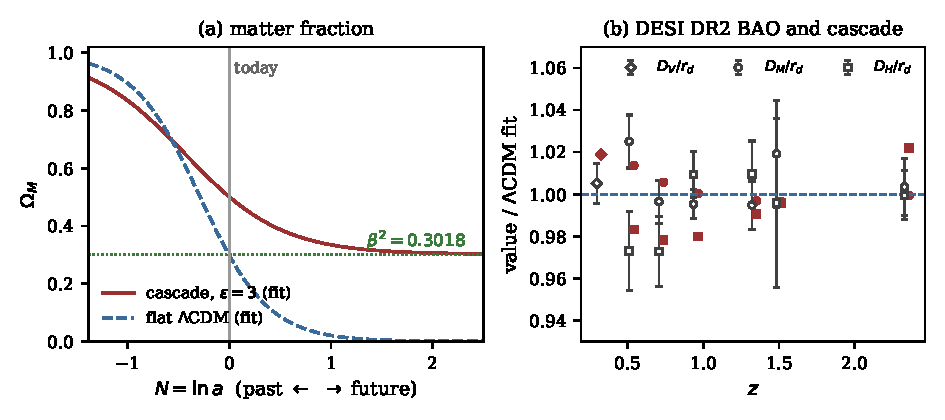
\includegraphics[width=\textwidth]{figures/F10-attractor.pdf}
\caption{Cascade with attractor $\Omega_M=\beta^2$ (H124).  (a) Matter fraction against $N=\ln a$ for the best-fitting cascade with
$\varepsilon=3$ ($\Omega_{M0}=0.5006$) and for flat $\Lambda$CDM ($\Omega_m=0.2970$), both fitted to DESI DR2 BAO \cite{DESIDR2}; the cascade
approaches $\beta^2=0.3018$ only in the future.  (b) The 13 BAO values (open symbols, $1\sigma$ diagonal errors) and the cascade prediction (filled,
slightly offset in $z$), each divided by the $\Lambda$CDM fit; each model has its own fitted $hr_d$.  Generated by
\texttt{scripts/F10\_attractor.py} from the data and model code of the H97/H124 tests in the Companion notes, which reproduces
$\chi^2_{\min}=18.42$ and $\Delta\chi^2=7.87$.  Status: H124 not excluded by BAO, not blind; the attractor does not fix the epoch.}
\label{fig:lop5-attractor}
\end{figure}

\subsection{Summary}
\label{sec:lop5-summary}

\begin{center}\small
\begin{tabular}{@{}p{0.48\textwidth}p{0.44\textwidth}@{}}
\toprule
statement & status\\
\midrule
H96: $\Omega_M=\bsym^2=0.30185$ today & \Open; decided by DESI DR3 or Euclid\\
H97: cascade bridge with $\varepsilon=1$ & \Refuted\ ($p=6\times10^{-17}$)\\
compact ordinary response of a prepared source & \Established\ (r32.3)\\
directed contrast on the same axis & \Conditional\ on a source identification without action\\
directed coupling with the luminal Higgs radius of W2 & \Refuted: violates the cone limit for every mediator\\
directed coupling in vacuum & $g_m^2\lesssim10^{-26}$ under the laboratory bound\\
$\Lambda$ within $\mathcal K$ & input; equivalent to the epoch of the readout\\
H124: attractor at $\varepsilon=3$ & not excluded by BAO ($p=0.072$), $\Omega_{M0}\approx0.50$, $\Delta\chi^2=7.87$\\
OP5 & \Open; core closure only as a conditional schema\\
\bottomrule
\end{tabular}
\end{center}

% Section 9 (group D): open problems and testable statements.
% Sources: Companion rounds v4.10.0-r05, r08, r18, r21, r28, r30, r31, r55, r56, r59, r60, r72--r75;
% wiki/Vorhersagen-und-Tests.md, wiki/Offene-Probleme.md, wiki/Gesamtbild.md.
\section{Open problems and testable statements}
\label{sec:open}

\subsection{The open problems}
\label{sec:open-problems}

The Companion names five open problems OP1--OP5 and two closure questions, C5 and C6/T2. None of them is closed
\cite{QSC}. Their present formulation is best read through one observation of \rnd{r30} and \rnd{r55}: every number that
OP2--OP5 supply today is a function of the single number of OP1, $\bsym=0.5494$, but it enters each problem through a
separately set identification, four of them chosen after the data were known (\rnd{r30}, remark r30.6). Each problem
also keeps a remainder that does not depend on the number (\rnd{r55}, remark r55.4).

\paragraph{OP1: the origin of $\bsym$.} \Open\ The frame offset is computed from a counting rule that is postulated, not derived (\rnd{r67}):
\begin{equation}
\bsym=\sqrt{\frac{\gamma_L-1}{\gamma_L+1}}=0.5494,\qquad \gamma_L=\frac{\gamma_M}{\gamma_T}=1.8647,
\label{eq:open-beta}
\end{equation}
where $\gamma_M=0.237533$ is the
Barbero--Immirzi value of the counting rule with all spins and weight two (assigned to frame M) and
$\gamma_T=\ln2/(\pi\sqrt3)=0.127384$ that of the rule with $j=\tfrac12$ only (assigned to frame T). The assignment is
equivalent to a frame-dependent area quantum (\rnd{r10}). Unitary boosts leave the area spectrum fixed, the Holst duality
rotation does not map $\gamma_M$ to the needed value, and the non-unitary frame map $J_B$ is a conjugation that leaves every
spectrum fixed (\rnd{r30}, \rnd{r31}, \rnd{r52}). OP1 therefore rests on the counting rules alone: why M counts every spin with
weight two, the extremal doublet of each puncture (the premise called U2) and why T counts only $j=\tfrac12$. Both premises and the Casimir area $\sqrt{j(j+1)}$ form the counting postulate adopted by the author on 26 November 2026 (\rnd{r67});
with the area $j+\tfrac12$ the same rule would give $1/\sqrt3$. The postulate replaces two literature values by one rule with three named
parts and leaves OP1 open in the form ``derive the counting postulate''. A solution would supply the
number but none of the five identifications (\rnd{r55}, r55.1). Section~\ref{sec:beta} gives the details.

\paragraph{OP2: the Dirac operator on the antisymmetric sector.} \Open\ Existence and self-adjointness of the operator $D_-$
on the antisymmetric sector were derived from an earlier manuscript of the author, which has not been a source of proof since v4.8.0-r04.
Its own remainder is that proof; its identification with the frame offset (spectral offset $=\bsym$) is one of the five
set translations (\rnd{r30}, r30.6).

\paragraph{OP3: generations and the residual bend.} \Open\ The Companion does not derive three generations, has no ban on
a fourth, and does not derive Koide's $K=2/3$; the overlap $\tfrac12$ is an input (Section~\ref{sec:B-koide}). Its number-dependent part is
the residual bend $\Phi_e=\pi/4-\gamma_M/2$ of the lepton phase, tested by H102. The orientation of the octant step is a
time orientation of the readout that no candidate of the Companion fixes (H118); on this the author decided on 22~November
2026 to let OP3 rest until a new idea appears (\rnd{r31}, r31.2). The Albert-algebra route gives a family $SO(3)$ broken by charge
exactly to $A_4$, with $V_{\mathrm{CKM}}=\mathbf 1$ for exact $A_4$, but no numbers (\rnd{r60}; Section~\ref{sec:B-particles}).
After \rnd{r60} two of these questions were answered without closing OP3 (tests H138--H156 of 25 and 26~November 2026, partly
not blind; recorded in Companion rounds \rnd{r62}, \rnd{r63}). The three $G_2$-stable octonion copies in the sedenions share one colour
$su(3)$ and have no common charge: they are three readings of one generation, not three generations (H138, H140); the number of generations stays an input. In an
amplitude readout $K=1/(3\cos^2\theta)$, so $K=\tfrac23$ holds exactly at the mixing angle $\theta=\pi/4$, the fixed point of
a swap read as the exchange of matter and tachyon frame (H148, H149); the swap symmetry is a postulate that the algebra
does not supply (H156), and the phase $\delta=2/9$ remains a fit. Rounds \rnd{r73} and \rnd{r74} reduce it to one set sign and one
rotation angle, $\varphi_\ell=0.0395773$, which no route tried derives and which stays a measured input (Section~\ref{sec:B-lepton-phase}).

\paragraph{OP4: the origin of the mixing angles.} \Open\ Several constructions reproduce the mixing data, but as fits.
The translations of the number are $|U_{e2}|^2=\bsym^2$ (H9) and the mask parameter $\varepsilon=\eta$ (H46). The own
remainder is the $\mathbb Z_2$ of the neutrinos (TM2), $\delta_{\mathrm{CP}}$, the CKM matrix and the assignment of gauge
charges (\rnd{r55}). One relative sign follows from the structure once the same side of the multiplication is taken
for the family in both sectors (\rnd{r65}): the relative orientation of the family $su(2)$ on leptons and quarks (H125 stage A, not blind), which under a
further setting S1 becomes the prediction $\sin\delta_{\mathrm{PMNS}}<0$ (\rnd{r59}).

\paragraph{OP5: the cosmological constant and the vacuum balance.} \Open\ By an author decision OP5 has three parts
(\rnd{r05}, r05.3): the core closure of the source--return route, locally closed under the guards and not claimed
globally; the $\Lambda$ readout $\Omega_M=\bsym^2$ (H96, open); and the action programme W1/W2, frozen
(Section~\ref{sec:act}). The own remainder, the absolute value of $\Lambda$, is an input for the named class of
constructions of the Companion: no equation in it selects $\Lambda$ and the class has no scale of its own; the readout
$\Omega_M=\bsym^2$ only trades $\Lambda$ for the epoch (\rnd{r56}). This is a negative result for the Companion as it
stands, not for every extension (Section~\ref{sec:lop5}).

\paragraph{C5.} \Open\ In its old form C5 asked, in the measure of one frame, about a passage between two frames. It was
restated in \rnd{r21} as three questions. The transfer question $C5_{\mathrm{tr}}$, typed by frame, is, within the reading of \rndold{r10}, a relocation: an
empty compensator port is a full partner port, since $C5_M+C5_T=1$; nothing vanishes. The frame-free photon-point
question $C5_P$ has a positive answer as a statement about fields: free time evolution reaches $|s|=0$ at a finite time
on a codimension-one family. Only the bridge question $C5_{\mathrm{br}}$, whether reaching the photon point discharges the
obstruction, is open; under the original definition of the score its answer is negative (r21.12), and the assertion
$C5=0$ is not made.

\paragraph{C6/T2 and the guards.} The global closure of all readouts, C6/T2, is \emph{not claimed}. The Companion
asserts only local, frame-typed closures (thesis T15). Its five guards are unchanged: every round up to \rnd{r75} records
$R_{\mathrm{glob}}=(0,1,1,1,1)$, $\Gamma_{\mathrm{guard}}=(1,1,1,1,1)$ and the end bound $\beta_4=1/256$ unspent, and states that it
implies no exact finite C5 zero closure, no exact all-readout terminality, no C6/T2, no global photon-clock theorem and no
global all-readout closure. Round \rnd{r72} restates the fourth guard, unchanged in content and value, as ``no global photon-clock
theorem''.

\subsection{Testable statements}
\label{sec:open-tests}

The Companion fixes each prediction in a pre-registration note (hypothesis, data, decision criterion) committed before
the decisive data exist; a value counts as tested only with a measurement after the stated cutoff, and earlier data are
given for comparison only. Table~\ref{tab:open-tests} lists the predictions that are open, together with H2. The status is
that of 25~November 2026; the dated list of this version, with the neutrino masses of H227 and the mixing readings recorded after
that date, is Table~\ref{tab:open-predictions}. None of the open tests is decided. One further open pre-registration is in no Companion round up to
\rnd{r61} and not in the table: H105 (horizon area steps $4\ln2\,\ell_P^2$ and ringdown echoes under an added setting V1,
deadline 31.12.2028; recorded in \rnd{r64}); its value is not specific to the construction.

\begin{table}[ht]
\centering
\footnotesize
\renewcommand{\arraystretch}{1.15}
\begin{tabularx}{\textwidth}{@{}l>{\raggedright\arraybackslash}p{0.27\textwidth}>{\raggedright\arraybackslash}X>{\raggedright\arraybackslash}p{0.25\textwidth}@{}}
\toprule
& statement & decisive data; refuted if & status and remarks\\
\midrule
H2 & normal ordering, $\sum m_\nu=0.0592$\,eV (neutrinos as light-like triple) & mass ordering and $\sum m_\nu$ &
  compatible, weakly discriminating; ordering not yet determined (\rnd{r18})\\
H9 & $\sin^2\theta_{12}=\bsym^2/\cos^2\theta_{13}=0.3086$ & JUNO with $\sigma\le0.004$ &
  open; found after the fact; JUNO 2026: $0.3036\pm0.0064$ (\rnd{r31})\\
H15 & $m_W=80.3615\pm0.0018$\,GeV & first world average after 21.10.2026 &
  open; PDG 2026 ($80.3625\pm0.0077$) predates H15 and does not count (\rnd{r04})\\
H42 & $\sin^2\theta_{23}\le0.54$ (normal ordering) & first global analysis or DUNE/Hyper-K result after 24.10.2026; refuted if the
  $2\sigma$ interval lies wholly above $0.54$ & open; independent of $\gamma_L$ (\rnd{r08})\\
H46 & $\sin^2\theta_{23}\in[0.49,0.50]$ under $\varepsilon=\eta$ & same data; refuted if the $2\sigma$ interval misses $[0.49,0.50]$ &
  open\\
H96 & $\Omega_M=\bsym^2=0.30185$ today & first flat-$\Lambda$CDM $\Omega_m$ from DESI DR3 (BAO alone) or Euclid; refuted beyond $2\sigma$ &
  open; DESI DR2 $0.2975\pm0.0086$ known, does not count (\rnd{r05})\\
H100 & $R=\Delta m^2_{21}/\Delta m^2_{31}$ in the next NuFIT fit: A $0.030839$, B $0.030087$, C $0.030375$ & first NuFIT version after 6.1;
  confirmed if A is refuted and B or C compatible ($|z|\le2$); lapses without a new version by end of 2027 & open (\rnd{r12})\\
H102 & $m_\tau=1777.134$\,MeV from $\Phi_e=\pi/4-\gamma_M/2$ (exact Koide: $1776.969$) & first PDG edition after 13.11.2026, at the
  latest end of 2028; refuted if $|z|>2$ & open; $+2.3\sigma$ against PDG 2024, $1776.93\pm0.09$, unchanged in PDG 2026 (\rnd{r28}.3); exact Koide lies at $+0.4\sigma$\\
H112 & $\sin^2\theta_{12}\cos^2\theta_{13}=\Omega_m$, the same number at both places, whatever it is & data of H9 and H96 together;
  refuted if $|z|\ge3$; deadline 31.12.2029 & open; weak (refutes only from $|\Delta\beta^2|\gtrsim0.022$)\\
H125 & $\sin\delta_{\mathrm{PMNS}}<0$ (relative CP sign of leptons and quarks, under S1 and the same-side setting) & first analysis fixing the sign at $\ge3\sigma$;
  deadline 31.12.2035 & open; stage A confirmed, \emph{not blind}; prior probability $\tfrac12$ (\rnd{r59}); NuFIT fits already
  lean to $\sin\delta<0$\\
\bottomrule
\end{tabularx}
\caption{Open pre-registered predictions of the Companion rounds, and H2, status of 25 November 2026 (wiki page ``Vorhersagen und
Tests'' and the cited rounds). H15, H46 and H96 rest on one common core, the assignment of counting rules to the frames;
H102 is a joint test of the core reading, the $U(1)$ counting and the area spectrum $\sqrt{j(j+1)}$.}
\label{tab:open-tests}
\end{table}

Three qualifications belong to every entry. First, the values of H9, H15, H46, H96 and H102 depend on the number of OP1, and
the chance estimate of Section~\ref{sec:beta} applies to them: as long as the pair of counting rules is chosen rather than derived, its
hits are compatible with chance. H15, H46 and H96 are not three independent tests; together with H42 the four older
predictions form two independent groups (\rnd{r08}). Second, H9 and H102 were found after the older data were seen; they
are blind only against future measurements. Third, H112 tests the weaker statement that the same number stands at both
places.

\Open\ \textbf{No blind prediction of the Companion has so far been confirmed against measurement data.} The confirmed
tests without the mark ``not blind'' all check inner mathematics (\rnd{r05}, remark r05.2), and no later test, up to
\rnd{r75}, has changed this. The predictions above and in Section~\ref{sec:open-predictions} are the places where that can change.

\subsection{Predictions of this version (as of 28 November 2026)}
\label{sec:open-predictions}

This version of the article (1.2.0) states the model of Companion v5.6.0 (Version DOI
\href{https://doi.org/10.5281/zenodo.24632437}{10.5281/zenodo.24632437}; predecessor v5.5.0, 10.5281/zenodo.24563811), as of
28~November 2026. Table~\ref{tab:open-predictions} collects its predictions. The full dated register, with deciding experiments, deadlines
and refutation criteria, is round \rnd{r75} of the Companion, which is authoritative; the binding criteria stand in the advance notes
of the tests. The last column says what each value rests on: \emph{derived} means computed from the stated inputs, \emph{set} a postulate
or a setting, \emph{measured} a measured input or a scale fitted to data, \emph{post hoc} a relation found after the data were known.
Common to all lepton rows: the Brannen form \eqref{eq:B-brannen-sector} is set; $K=\tfrac23$ holds under the postulate of equal standing
of the frames; $\varphi_\ell=0.0395773$ is a measured input; the sign of the branch choice is a setting; the scales $\mu_e$, $\mu_\nu$
are fitted. Common to the rows that use $\bsym$: the value $\bsym=0.5494056410$ is computed from the counting postulate of \rnd{r67}
and is not derived.

\begin{table}[htp]
\centering
\footnotesize
\renewcommand{\arraystretch}{1.12}
\begin{tabularx}{\textwidth}{@{}>{\raggedright\arraybackslash}p{0.15\textwidth}>{\raggedright\arraybackslash}p{0.26\textwidth}>{\raggedright\arraybackslash}p{0.12\textwidth}>{\raggedright\arraybackslash}X@{}}
\toprule
quantity & prediction & source & rests on\\
\midrule
mass ordering & normal & H227, H213; \rnd{r73} & derived from $\varphi_\ell$ (measured); branch sign and Brannen form set\\
$\sum m_\nu$ & $59.30\pm0.24$\,meV & H227; \rnd{r73} & derived; $\varphi_\ell$ measured, $\mu_\nu$ fitted to $\Delta m^2_{31}$; $K=\tfrac23$ postulate; form and sign set\\
$m_1$, $m_2$, $m_3$ & $0.379$, $8.81$, $50.11$\,meV & H227; \rnd{r73} & as for $\sum m_\nu$\\
$m_\beta$ & $8.87$\,meV & H227; \rnd{r73} & as for $\sum m_\nu$; mixing data measured\\
$m_{\beta\beta}$ & $1.3$ to $4.0$\,meV (Majorana phases free) & H227; \rnd{r73} & as for $m_\beta$\\
$R=\Delta m^2_{21}/\Delta m^2_{31}$ & $0.030839$ (data $+1.8\sigma$; not blind) & H99, H100, H227 & derived from $\varphi_\ell$ (measured); sector assignment H99 and form set\\
$\sin^2\theta_{12}$ & three exclusive readings: $0.3086$; $0.3019$; $0.318$ to $0.3195$ & H9; H176; H206--H208 & H9: $\bsym^2$ (postulate), found post hoc; H176: one-number candidate with set readouts, selected post hoc; H206--H208: column $|U_{e1}|^2=\tfrac23$ derived, readout set\\
$\theta_{12}$--CP correlation & $\sin^2\theta_{12}\gtrsim0.315$ with $|\sin\delta|\approx1$, or $\sin^2\theta_{12}$ near $0.304$ with $|\sin\delta|\approx0.65$ & H206--H208 (JUNO with DUNE) & structural readout set; additional term allowed, not derived; correlation found post hoc (H208)\\
$\sin^2\theta_{23}$ & $0.4954$ (H176); $\le0.54$ (H42); $[0.49,0.50]$ (H46) & H176; H42, H46 & set readouts; $\bsym$ from the postulate (H46)\\
$\sin^2\theta_{13}$ & $0.0223$ (H176); $0.0216$ without parameter (H207) & H176, H207 & set readouts; H207 partly not blind\\
$\delta_{\rm CP}$ & $|\sin\delta|\approx0.977$ and $\sin\delta<0$, together about $282^\circ$ & H176; H125 & modulus as for $\theta_{23}$; sign rests on setting S1 and the same-side setting\\
$\Omega_m$ (flat $\Lambda$CDM) & $\bsym^2=0.30185$ & H96 & $\bsym$ from the postulate; identification $\Omega_M=\bsym^2$ set\\
$m_W$ & $80.3615\pm0.0018$\,GeV & H15 & $\gamma_L$ from the postulate; $\cot\theta_W=\gamma_L$ set, found post hoc; $m_Z$ measured\\
$m_\tau$ & $1776.969$\,MeV (Koide; not blind); alternative $1777.134$\,MeV & \rnd{r63}, H227; H102 & $K=\tfrac23$ postulate, $m_e$, $m_\mu$ measured; the alternative rests on the bent-octant placeholders, found post hoc\\
\bottomrule
\end{tabularx}
\caption{Predictions of version 1.2.0, as of 28 November 2026 (Companion v5.6.0, round \rnd{r75}). The rows are not independent: H15,
H46 and H96 share the counting core; H9, H96 and H112 share $\bsym^2$; the three readings of $\theta_{12}$ exclude one another.}
\label{tab:open-predictions}
\end{table}

\paragraph{Version rule.} By a standing rule of the author (28 November 2026; \rnd{r75}.1) every public version records its predictions
with date and DOI. These numbers are fixed with this version and are not readjusted after a new measurement. A correction appears only in
a later version, with its reason stated (progress of the model or an error). The version that was fixed before the measurement counts as
the test, and earlier versions stay visible under their DOIs. Several rows fall together: an established inverted ordering or a measured
$\sum m_\nu<58$\,meV refutes the mass balance and with it the Brannen form for neutrinos; JUNO separates the three readings of
$\theta_{12}$ and, with DUNE, tests the correlation; a deviation of $\Omega_m$ or $m_W$ bears on the counting postulate; the two values of
$m_\tau$ separate only at an uncertainty of about $0.05$\,MeV. The register adds no derivation, no guard is spent, and OP1--OP5, C5 and
C6/T2 remain open.

\section{Conclusion}
\label{sec:concl}

The construction delivers structure. The carrier, the compensator and the sector rule are exact; the frame maps are symmetries
that give equalities rather than values, together with the Lorentz group and scale they leave exactly two classes of fields
(light-like or not), and the tachyon map is distinct from time reversal. On the Dixon algebra the
choices that produce one generation are explicit, and the Albert algebra turns the charge into a precise breaking of a family
symmetry to $A_4$. Exclusions are part of this yield: one generation has no internal generation qubit, frame maps produce no
values, a unitary boost cannot change an area quantum, and within the present stock no equation fixes $\Lambda$.

The construction does not deliver numbers. The Koide value is a statement about three states with overlap $\tfrac12$, and that
overlap is put in; later tests relate it to a mixing angle $\pi/4$ at the fixed point of a frame swap that again has to be
postulated, and find the three octonion copies in the sedenions to be one generation read three ways (H138--H156, \rnd{r62}, \rnd{r63};
Section~\ref{sec:open-problems}). The lepton phase reduces to one rotation angle and one set sign; the angle, $0.0395773$, stays a measured
input; no route tried derives it (\rnd{r73}, \rnd{r74}). The conditional numbers of OP2--OP5 go back to $\bsym$
through separately set identifications, and $\bsym$ is computed from a counting rule that is adopted as a postulate and not derived (\rnd{r67}). The
common action W1/W2 is consistent and has no scale of its own. The Big Bang as a transition between two readings of one field is
an exploration.

The next step is therefore narrow. A derivation would have to supply one of three things: a reason for the counting rule per frame
(OP1), a structure that fixes the overlap $\tfrac12$ or the orientation of the octant, or a scale from the dynamics (a first
loop ansatz fixed none, Section~\ref{sec:act-noscale}). Until then the
open predictions of Table~\ref{tab:open-tests} and the dated predictions of this version in Table~\ref{tab:open-predictions} are the contact
with data, fixed before the measurements that will decide them; H42, H100, H112 and H125 are those whose outcome does not
rest on the value of $\bsym$.

\appendix
\section{Status ledger}
\label{sec:ledger}

The status of each statement is given where it is made. Four sections close with a status table:
Table~\ref{tab:A-summary} (carrier and frames), Table~\ref{tab:B-koide-tests} (tests on the Koide geometry),
Table~\ref{tab:act-status} (action W1/W2) and the summary of Section~\ref{sec:lop5}; the open predictions are collected in
Table~\ref{tab:open-tests}. Table~\ref{tab:ledger} adds the main statements of Sections~\ref{sec:B-particles},
\ref{sec:B-koide} and~\ref{sec:beta} in the same form. ``Not blind'' means that the result or the data were known before the
pre-registration note was committed.

\begin{table}[h]
\centering\small
\begin{tabularx}{\textwidth}{@{}>{\raggedright\arraybackslash}X l l@{}}
\toprule
statement & status & source\\
\midrule
one generation and the Standard Model gauge group on $\mathbb C\otimes\mathbb H\otimes\mathbb O$ & \Conditional{} (Table~\ref{tab:B-choices}) & \rndold{r34}--\rndold{r49}\\
no ban on a fourth generation & \Open & \rndold{r37}\\
commutant of gauge and Lorentz group on one generation is $\mathbb C^6$ & \Established & \rnd{r19}\\
route A (sedenions, charge axis $e_8$): $2T$ on a neutral qubit, two generations & \Conditional{} (CT-003) & \rnd{r13}\\
route B ($\mathbb O^3$, triality): three slots, no magic angle & \Established{} as algebra & \rnd{r13}\\
Albert algebra: family $SO(3)$ broken by the charge operator to $A_4$, pure spin 3 & \Established{} (H127 stage A) & \rnd{r60}\\
relative CP sign of leptons and quarks & \Conditional{} on CT-003 (H125 stage A, not blind) & \rnd{r59}\\
$\sin\delta_{\rm PMNS}<0$ & \Open{} (deadline 2035) & \rnd{r59}\\
absolute handedness & convention (choice of $i$) & \rnd{r59}\\
\midrule
$K=(1+2\rho^2)/3$; $K=\tfrac23\Leftrightarrow\rho^2=\tfrac12$ & \Established & \rnd{r12}\\
overlap $\tfrac12$, hence $K=\tfrac23$, from the construction & \Open{} (input) & \rnd{r12}, \rnd{r16}\\
bent octant, $\det G=(\sqrt2\cos\varphi-1)/2$ & \Established & \rnd{r14}\\
$K=2/(d+1)$; only $d=2$ gives three states & \Established & \rnd{r15}\\
at most three pairwise non-orthogonal readouts, forming the octants & \Established & \rnd{r16}\\
guarded core as origin of the bend & \Reading & \rnd{r14}, \rnd{r28}\\
orientation of the octant step & \Open{} (time orientation of the readout) & \rnd{r30}, \rnd{r31}\\
\midrule
$\beta=\sqrt{(\gamma_L-1)/(\gamma_L+1)}$ as algebra of the symmetric frame & \Established & \texttt{thm:symmetric-frame}\\
$\bsym=0.5494$ as a physical frame offset & \Conditional{} (U(1) counting per frame) & \rnd{r08}\\
special position of the counting-rule pair (H98) & confirmed, not blind & \rnd{r09}\\
frame-dependent area quantum under unitary boosts & excluded (Rovelli--Speziale) & \rnd{r30}\\
$\gamma_L$ from duality rotations of the Holst term & excluded (\Established{} within W1 plus Holst) & \rnd{r31}\\
temporal octant readout as counting rule (H123d) & \Refuted & \rnd{r58}\\
origin of the counting rule per frame (OP1) & \Open & \rnd{r30}\\
\midrule
blind prediction confirmed against measurement data & none so far & \rnd{r05}, Section~\ref{sec:open}\\
\bottomrule
\end{tabularx}
\caption{Ledger of the main statements of Sections~\ref{sec:B-particles}--\ref{sec:beta}.}
\label{tab:ledger}
\end{table}

% Appendix B (group D): reproduction. Every path below was checked to exist in the repository on 25 November 2026 (H213--H236 folder on 28 November 2026).
\section{Reproduction}
\label{sec:repro}

\paragraph{Source version.} The article reports the Quantum Sphaera Companion \cite{QSC}. The baseline is v5.6.0
(28~November 2026, Version DOI \href{https://doi.org/10.5281/zenodo.24632437}{10.5281/zenodo.24632437}, Concept DOI
\href{https://doi.org/10.5281/zenodo.19210728}{10.5281/zenodo.19210728}; predecessor v5.5.0,
\href{https://doi.org/10.5281/zenodo.24563811}{10.5281/zenodo.24563811}); it contains the research rounds
up to v4.10.0-r75, among them r60, r61 (formula corrections), r62--r65 (the tests after r60 that are cited here: H105,
H128--H156 and H162), r66, r67 (H164, H165 and the counting postulate), r69 (names of the frames and lepton sectors), r70 (frames on
the state sphere), r72 (photon-clock guard restated), r73, r74 (lepton phase, H213--H236) and r75 (dated register of predictions).
The German preprint 0.5.0 \cite{QS-preprint-de} is built on the same Companion version. The sources are in the public repository
\url{https://github.com/Moriarty1982/QuantumSphere-Unfold}. Nothing after r75 is used. In that repository:
\begin{itemize}
\item \nolinkurl{sources/research/v480-companion.tex} is the entry point of the Companion (historical file name);
\item \nolinkurl{sources/research/parts/v490-post-release-layers.tex} holds the rounds v4.9.0-r01 to r86, cited here as
  \textsc{c}\,4.9-rNN;
\item \nolinkurl{sources/research/parts/v4100-post-release-layers.tex} holds the rounds v4.10.0-r01 to r75, cited as
  \textsc{c}\,rNN, with labels \texttt{sec:v4100-rNN-\dots}.
\end{itemize}
Each round ends with a ledger and guard update and names its notes and scripts, in a ``Proof and measurement
sources'' paragraph or, in most later rounds, in the results or in a closing notes paragraph.

\paragraph{Where the scripts live.} The notes of a round are in \nolinkurl{notes/research/v4_10_0_rNN/}. The folder name
follows the working sequence, not the round label: \nolinkurl{v4_10_0_w1/} holds the notes of v4.9.0-r81,
\nolinkurl{v4_10_0_r82/} to \nolinkurl{v4_10_0_r86/} those of v4.9.0-r82 to r86, and \nolinkurl{v4_10_0_r01/} onwards those
of v4.10.0-r01 onwards. Scripts and their recorded outputs are in the subfolder \nolinkurl{llm/} or, for later rounds, in a
topic folder that the round's \texttt{README.md} names (for example \nolinkurl{notes/research/op5_attractor_2026_11_23/} for
H124 and \nolinkurl{notes/research/h125_relatives_cp_2026_11_24/} for H125). Pre-registration and result notes
(\nolinkurl{Vorab_Notiz_H*.md}, \nolinkurl{Ergebnis_H*.md}) are in \nolinkurl{notes/research/predictions/} for H42, H46,
H48--H112 and H124--H137, in the \nolinkurl{llm/} folder of their round for earlier tests, in \nolinkurl{llm/} at the top
level for H113--H123 and in \nolinkurl{notes/research/hilbert_shift_felder_2026_11_24/} for H138--H156 and, with one subfolder per test, for H213--H236
(scripts k426--k451 with Wolfram cross-checks; folder list in \rnd{r73} and \rnd{r74}). The commit of a pre-registration note can be compared with the date of the computation. Table~\ref{tab:repro-act} lists the scripts
behind the numbers of Section~\ref{sec:act}.

\begin{table}[ht]
\centering
\footnotesize
\begin{tabularx}{\textwidth}{@{}>{\raggedright\arraybackslash}p{0.33\textwidth}>{\raggedright\arraybackslash}X l@{}}
\toprule
result & script (path under \nolinkurl{notes/research/}) & tool\\
\midrule
$\mathrm{Im}\,S$ identity of the complex reading & \nolinkurl{v4_10_0_w1/llm/k170_imS_identitaet.py} & Python\\
vacuum decay of an independent T field (H76) & \nolinkurl{v4_10_0_r83/llm/k191_vakuumzerfall.py} & Python\\
second reading on FRW (H80, H81) & \nolinkurl{v4_10_0_r84/llm/k196_zweite_lesart_frw.py} & Python\\
masses under the second reading (H82) & \nolinkurl{v4_10_0_r85/llm/k197_massen_zweite_lesart.py} & Python\\
CPT assignment at the Big Bang (H86) & \nolinkurl{v4_10_0_r85/llm/k201_cpt_zuordnung.py} & Python\\
admixture, second system (H87) & \nolinkurl{v4_10_0_r86/llm/k202_wolfram_gegenprobe.wl} & Wolfram\\
field equations of W1 (H88) & \nolinkurl{v4_10_0_r86/llm/k203_w1_feldgleichungen.wl} & Wolfram\\
energy--momentum tensor of W1 (H89) & \nolinkurl{v4_10_0_r86/llm/k204_w1_einstein.wl} & Wolfram\\
non-linear Einstein--Cartan equation, sign (H90) & \nolinkurl{v4_10_0_r01/llm/k205_w1_einstein_nichtlinear.py},
  output \nolinkurl{k205_out.json} & Python (jets)\\
weak-field sign check & \nolinkurl{v4_10_0_r01/llm/k205b_schwachfeld.wl} & Wolfram\\
fermions at the Big Bang & \nolinkurl{v4_10_0_r03/llm/k209_fermionen_urknall.py}, output \nolinkurl{k209_out.txt} & Python (sympy)\\
the two senses of rotation & \nolinkurl{v4_10_0_r03/llm/k211_symmetrie_drehsinne.py}, output \nolinkurl{k211_out.txt} & Python\\
branch gas on FRW (H95) & \nolinkurl{v4_10_0_r04/llm/k212_zweiggas_frw.py}, output \nolinkurl{k212_out.json} & Python\\
\bottomrule
\end{tabularx}
\caption{Scripts behind Section~\ref{sec:act}. The Wolfram files of \texttt{v4\_10\_0\_r86/\allowbreak llm/\allowbreak } have no separate output
files; their results and the disclosed errors of the checking code are recorded in
\texttt{predictions/\allowbreak Ergebnis\_H87\_*}, \texttt{Ergebnis\_H88\_*} and \texttt{Ergebnis\_H89\_*}.}
\label{tab:repro-act}
\end{table}

\paragraph{Tools.} Numerical work uses Python (NumPy, SciPy, sympy for symbolic steps). Wolfram Language is used for exact
and symbolic derivations and as an independent second system, as in the derivation of the field equations of W1 and the
recomputation of the Big Bang admixture (\rndold{r86}). A separate Wolfram audit archive with input scripts and recorded
outputs for the algebraic core, the Dixon carrier, the Koide geometry and the OP5 comparison model is in
\nolinkurl{paper/preprint-de/audit/wolfram-v0.1.0/}. Round labels, cross references, guards and the ledger are checked with
\nolinkurl{tools/qs.py}.

\paragraph{Rebuilding.} The article is self-contained in \nolinkurl{paper/physics-standalone/}: \texttt{article.tex} with
\nolinkurl{sections/}, the TikZ figures in \nolinkurl{figures/} and the bibliography in \nolinkurl{refs/}. Run \texttt{pdflatex
article.tex} twice in that directory; scripts that generate figure data are in \nolinkurl{scripts/}. The Companion is built
from \nolinkurl{sources/research/v480-companion.tex} with that directory as working directory and several pdfLaTeX runs, as
described in \nolinkurl{sources/research/README.md}.


\begin{thebibliography}{99}
\bibitem{QSC}
M.~Brendecke, \emph{Quantum Sphaera Companion: A Structure-First Mathematical
Unfolding}, v5.5.0 (2026), doi:10.5281/zenodo.24563811; rounds up to v4.10.0-r68, sources in
\url{https://github.com/Moriarty1982/QuantumSphere-Unfold}, \texttt{sources/research/}.

\IfFileExists{refs/A.tex}{% References used in Sections 1-3 (group A).
\bibitem{A-DorauMuch2026}
P.~Dorau and A.~Much, \emph{From Quantum Relative Entropy to the Semiclassical Einstein Equations},
Phys.\ Rev.\ Lett.\ \textbf{136}, 091602 (2026), doi:10.1103/lmq8-nsty, arXiv:2510.24491.

\bibitem{A-Jacobson1995}
T.~Jacobson, \emph{Thermodynamics of Spacetime: The Einstein Equation of State},
Phys.\ Rev.\ Lett.\ \textbf{75}, 1260 (1995), doi:10.1103/PhysRevLett.75.1260.

\bibitem{A-BBB2013}
I.~Bialynicki-Birula and Z.~Bialynicka-Birula, \emph{The role of the Riemann--Silberstein vector in
classical and quantum theories of electromagnetism}, J.\ Phys.\ A \textbf{46}, 053001 (2013), arXiv:1211.2655.

\bibitem{A-Golat2024}
S.~Golat, A.~J.~Vernon and F.~J.~Rodr\'iguez-Fortu\~no, \emph{The electromagnetic symmetry sphere: a framework for
energy, momentum, spin and other electromagnetic quantities}, arXiv:2405.15718 (2024).
}{}
\IfFileExists{refs/B.tex}{% Group B references (sections 4 and 5). Bibliographic data taken from the Companion (v4.10.0-r19.3, r19.4)
% and from paper/preprint-de/article.tex.
\bibitem{Dixon1994}
G.~M.~Dixon, \emph{Division Algebras: Octonions, Quaternions, Complex Numbers and the Algebraic Design of Physics},
Kluwer, Dordrecht (1994).

\bibitem{Furey2015}
C.~Furey, \emph{Charge quantization from a number operator}, Physics Letters B \textbf{742} (2015), 195--199.

\bibitem{Koide1983}
Y.~Koide, \emph{A fermion-boson composite model of quarks and leptons}, Physics Letters B \textbf{120} (1983), 161--165.

\bibitem{Brannen2010}
C.~A.~Brannen, Foundations of Physics \textbf{40} (2010), 1681, arXiv:1006.3114.

\bibitem{Foot1994}
R.~Foot, arXiv:hep-ph/9402242 (1994).

\bibitem{Zenczykowski2012}
P.~\.Zenczykowski, Physical Review D \textbf{86} (2012), 117303; Physical Review D \textbf{87} (2013), 077302.

\bibitem{Golat2024}
Golat, Vernon and Rodr\'iguez-Fortu\~no, arXiv:2405.15718 (2024).
}{}
\IfFileExists{refs/C.tex}{% Group C references (sections 6 and 8)
\bibitem{ABCK1998}
A.~Ashtekar, J.~Baez, A.~Corichi and K.~Krasnov, \emph{Quantum geometry and black hole entropy},
Phys.\ Rev.\ Lett.\ \textbf{80} (1998) 904, arXiv:gr-qc/9710007.

\bibitem{DomagalaLewandowski2004}
M.~Domaga{\l}a and J.~Lewandowski, \emph{Black-hole entropy from quantum geometry},
Class.\ Quantum Grav.\ \textbf{21} (2004) 5233, arXiv:gr-qc/0407051.

\bibitem{Meissner2004}
K.~A.~Meissner, \emph{Black-hole entropy in loop quantum gravity},
Class.\ Quantum Grav.\ \textbf{21} (2004) 5245, arXiv:gr-qc/0407052.

\bibitem{GhoshMitra2005}
A.~Ghosh and P.~Mitra, \emph{An improved estimate of black hole entropy in the quantum geometry approach},
Phys.\ Lett.\ B \textbf{616} (2005) 114, arXiv:gr-qc/0411035.

\bibitem{EngleNouiPerez2010}
J.~Engle, K.~Noui and A.~Perez, \emph{Black hole entropy and SU(2) Chern--Simons theory},
Phys.\ Rev.\ Lett.\ \textbf{105} (2010) 031302, arXiv:0905.3168.

\bibitem{FroddenGhoshPerez2013}
E.~Frodden, A.~Ghosh and A.~Perez, \emph{Quasilocal first law for black hole thermodynamics},
Phys.\ Rev.\ D \textbf{87} (2013) 121503, arXiv:1110.4055.

\bibitem{RovelliSpeziale2003}
C.~Rovelli and S.~Speziale, \emph{Reconcile Planck-scale discreteness and the Lorentz--Fitzgerald contraction},
Phys.\ Rev.\ D \textbf{67} (2003) 064019, doi:10.1103/PhysRevD.67.064019, arXiv:gr-qc/0205108.

\bibitem{Holst1996}
S.~Holst, \emph{Barbero's Hamiltonian derived from a generalized Hilbert--Palatini action},
Phys.\ Rev.\ D \textbf{53} (1996) 5966, arXiv:gr-qc/9511026.

\bibitem{DESIDR2}
DESI Collaboration, \emph{DESI DR2 Results II: Measurements of Baryon Acoustic Oscillations and Cosmological Constraints},
Phys.\ Rev.\ D \textbf{112} (2025) 083515, arXiv:2503.14738.

\bibitem{Planck2018}
Planck Collaboration, \emph{Planck 2018 results. VI. Cosmological parameters},
Astron.\ Astrophys.\ \textbf{641} (2020) A6, arXiv:1807.06209.

\bibitem{Altschul2010}
B.~Altschul, \emph{Laboratory bounds on electron Lorentz violation},
Phys.\ Rev.\ D \textbf{82} (2010) 016002, arXiv:1005.2994.
}{}
\IfFileExists{refs/D.tex}{% References used in Section 7, Section 9 and Appendix B (group D).
% Dixon's book is cited as Dixon1994 (entry in refs/B.tex).
\bibitem{D:HehlDatta}
F.~W.~Hehl and B.~K.~Datta, \emph{Nonlinear spinor equation and asymmetric connection in general relativity},
J.\ Math.\ Phys.\ \textbf{12}, 1334 (1971), doi:10.1063/1.1665738.

\bibitem{D:Cline}
J.~M.~Cline, S.~Jeon and G.~D.~Moore, \emph{The phantom menaced: constraints on low-energy effective ghosts},
Phys.\ Rev.\ D \textbf{70}, 043543 (2004), arXiv:hep-ph/0311312.

\bibitem{D:BFT}
L.~Boyle, K.~Finn and N.~Turok, \emph{CPT-symmetric universe}, Phys.\ Rev.\ Lett.\ \textbf{121}, 251301 (2018),
arXiv:1803.08928.
}{}
\end{thebibliography}
\end{document}
